\documentclass{article}

\usepackage{tikz-cd}
\usepackage{mathtools}
\usepackage[utf8]{inputenc}
\usepackage[english]{babel}
\usepackage{amsthm}
\usepackage{amsmath}
\usepackage{amssymb}
\usepackage{amsfonts}
\usepackage{marvosym}
\usepackage{hyperref}
\usepackage{amssymb}
\usepackage{graphicx}
\usepackage{titlesec}
\usepackage{cancel}

% amsthm definitions %
\newtheorem{proposition}{Proposition}[subsection]
\newtheorem{theorem}{Theorem}[subsection]
\newtheorem{corollary}{Corollary}[theorem]
\newtheorem{lemma}[theorem]{Lemma}


% titlesec definitions %
\titleclass{\subsubsubsection}{straight}[\subsection]

\newcounter{subsubsubsection}[subsubsection]
\renewcommand\thesubsubsubsection{\thesubsubsection.\arabic{subsubsubsection}}
\renewcommand\theparagraph{\thesubsubsubsection.\arabic{paragraph}} % optional; useful if paragraphs are to be numbered

\titleformat{\subsubsubsection}
  {\normalfont\normalsize\bfseries}{\thesubsubsubsection}{1em}{}
\titlespacing*{\subsubsubsection}
{0pt}{3.25ex plus 1ex minus .2ex}{1.5ex plus .2ex}

\makeatletter
\renewcommand\paragraph{\@startsection{paragraph}{5}{\z@}%
  {3.25ex \@plus1ex \@minus.2ex}%
  {-1em}%
  {\normalfont\normalsize\bfseries}}
\renewcommand\subparagraph{\@startsection{subparagraph}{6}{\parindent}%
  {3.25ex \@plus1ex \@minus .2ex}%
  {-1em}%
  {\normalfont\normalsize\bfseries}}
\def\toclevel@subsubsubsection{4}
\def\toclevel@paragraph{5}
\def\toclevel@paragraph{6}
\def\l@subsubsubsection{\@dottedtocline{4}{7em}{4em}}
\def\l@paragraph{\@dottedtocline{5}{10em}{5em}}
\def\l@subparagraph{\@dottedtocline{6}{14em}{6em}}
\makeatother

\setcounter{secnumdepth}{4}
\setcounter{tocdepth}{4}

\newcommand*{\LargerCdot}{\raisebox{-0.25ex}{\scalebox{1.5}{$\cdot$}}}

\title{Notes on Fundamental Concepts in Various Branches of Mathematics}
\author{Henry Fender}
\date{ }

\begin{document}

\maketitle
 
\tableofcontents

\section{Set Theory}\label{settheory}

\subsection{Set Axioms}\label{setaxioms}

\subsubsection{Undefined notions}
\emph{Set:} $A,B,C,\dots$

\subsubsection{Axioms}\label{statementofsetaxioms}
\begin{enumerate}
  \item \emph{Extension:} $\forall A \forall B [\forall C ( C \in A \Leftrightarrow C \in B ) \Rightarrow A = B ]$
  \item \emph{Regularity:} $\forall A [\exists C (C \in A) \Rightarrow \exists B ( B \in A \land \lnot \exists D (D \in B \land D \in A))]$ \newline
  {\small (Every nonempty set contains a set that is disjoint from it. Also know as "Axiom of Foundation.")}
  \item \emph{Schema of Specification:} $\forall B \forall X_1 \forall X_2 \dots \forall X_n \exists A \forall C [C \in A \Leftrightarrow ( C \in B \land \phi)]$
  \item \emph{Pairing:} $\forall X_1 \forall X_2 \exists A (X_1 \in A \land X_2 \in A)$
  \item \emph{Union:} $\forall \mathcal{F}_A \exists U \forall A \forall X [(X \in A \land A \in \mathcal{F}_A) \Rightarrow X \in U]$
  \item \emph{Schema of Replacement:} $\forall A \forall X_1 \forall X_2 \dots \forall X_n[\forall B(B \in A \Rightarrow \exists! D \phi) \Rightarrow \exists B \forall C (C \in A \Rightarrow \exists D(D \in B \land \phi))]$
  \item \emph{Infinity:} $\exists \omega_0 [\emptyset \in \omega_0 \land \forall X(X \in \omega_0 \Rightarrow X \cup X\} \in \omega_0)]$
  \item \emph{Power Set:} $\forall X \exists \mathcal{P}(X) \forall S [S \subseteq X \Rightarrow S \in \mathcal{P}(X)]$
  \item \emph{Empty Set:} $\exists A \forall X (X \not\in A)$
  \item \emph{Choice:} $\forall X [\emptyset \not\in X \Rightarrow \exists (f:X \rightarrow \bigcup X) \forall A \in X (f(A) \in A)]$
\end{enumerate}

\begin{proposition}
	The empty set axiom is implied by the other nine axioms.
\end{proposition}

\begin{proof}
	Just choose any formula that is always false such as $\phi(X) = X \in B \land X \not \in B$ and apply the axiom schema of specification. This
	will give the empty set. The axiom of extension proves uniqueness vacuously.
\end{proof}

\subsubsection{Universe}\label{universe}
A set $U$ is defined with the following properties\dots
\begin{enumerate}
  \item $x \in u \in U \Rightarrow x \in U$
  \item $u \in U \land v \in U \Rightarrow \{u,v\}, \langle u,v \rangle, u \times v \in U$
  \item $X \in U \Rightarrow \mathcal{P}(X) \in U \land \bigcup X \in U$
  \item $\omega_0 \in U$ is the set of finite ordinals
  \item if $f:A \rightarrow B$ is a surjective function with $A \in U \land B \subset U$, then $B \in U$
\end{enumerate}

(See: \hyperref[setconstructions]{Set Constructions}.)\newline

\noindent In category theory, \emph{small sets} are members of $U$. \label{smallsets}

\subsection{Set Constructions}\label{setconstructions}

\subsubsection{Union}\label{union}
\begin{itemize}
  \item $A\cup B := \{x | x \in A \lor x \in B \}$
  \item $\bigcup \mathcal{F} := \{x | x \in X \textrm{ for some } X \in \mathcal{F} \}$
\end{itemize}

\begin{proposition}
For sets $A,B,C$, the following hold\dots
\begin{itemize}
  \item \emph{Identity:} $A \cup \emptyset = A$
  \item \emph{Idempotence:} $A\cup A = A$
  \item \emph{Absorption:} $A \subseteq B \Leftrightarrow A \cup B = B$
  \item \emph{Commutative:} $A \cup B = B \cup A$
  \item \emph{Associative:} $A \cup (B \cup C) = (A \cup B) \cup C$
\end{itemize}
\end{proposition}
	
\subsubsection{Intersection}\label{intersection}
\begin{itemize}
  \item $A\cap B := \{x \in A | x \in B\} = \{x \in B | x \in A\}$
  \item $\bigcap \mathcal{F} := \{x | x \in X \textrm{ for all } X \in \mathcal{F} \}$
\end{itemize}

\begin{proposition}
For sets $A,B,C$, the following hold\dots
\begin{itemize}
  \item \emph{Zero:} $A \cap \emptyset = \emptyset$
  \item \emph{Idempotence:} $A\cap A = A$
  \item \emph{Absorption:} $A \subseteq B \Leftrightarrow A \cap B = A$
  \item \emph{Commutative:} $A \cap B = B \cap A$
  \item \emph{Associative:} $A \cap (B \cap C) = (A \cap B) \cap C$
\end{itemize}
\end{proposition}

\subsubsection{Complement}\label{complement}
\begin{itemize}
  \item \emph{Relative Complement:} $A \ensuremath{\setminus} B := \{x \in A | x \not\in B \}$
  \item \emph{Absolute Complement:} For some \hyperref[universe]{universe} $U$ and $A \subseteq U$, $A^{c} := U \ensuremath{\setminus} A$
\end{itemize}

\begin{proposition}
For a universe $U$ and sets $A,B \subseteq U$\dots
\begin{itemize}
  \item $(A^c)^c = A$
  \item $\emptyset^c = U$
  \item $U^c = \emptyset$
  \item $A \cap A^c = \emptyset$
  \item $A \cup A^c = U$
  \item $A \subseteq B \Leftrightarrow B^c \subseteq A^c$ 
\end{itemize} 
\end{proposition}

\begin{proposition}[DeMorgan's Laws]
For a universe $U$ and sets $A,B \subseteq U$\dots
\begin{itemize}
  \item $(A \cup B)^c = A^c \cap B^c$
  \item $(A \cap B)^c = A^c \cup B^c$
\end{itemize} 
\end{proposition}

\begin{proposition}
For sets $A,B$\dots
\begin{itemize}
  \item $A \setminus B = A \cap B^c$
  \item $A \subseteq B \Leftrightarrow A \setminus B = \emptyset$
  \item $A \setminus (A \setminus B) = A \cap B$
  \item $A \cap (B \setminus C) = (A \cap B) \setminus (A \cap C)$
  \item $A \cap B \subseteq (A \cap C) \cup (B \cap C^c)$
  \item $(A \cup C) \cap (B \cup C^c) \subseteq A \cup B$
\end{itemize}
\end{proposition}

\begin{proposition}
For a family $\mathcal{F}$\dots
\begin{itemize}
  \item $\forall X \in \mathcal{F}, \, \bigcup_{k \in K} X_k = \bigcup_{j \in J} (\bigcup_{i \in I_j} X_i)$
  \item $\forall X \in \mathcal{F}, \, \bigcap_{k \in K} X_k = \bigcap_{j \in J} (\bigcap_{i \in I_j} X_i)$
  \item $\forall X \in \mathcal{F}, \, \bigcup_{i \in I} X_i = \bigcup_{j \in J} X_j$
  \item $\forall X \in \mathcal{F}, \, \bigcap_{i \in I} X_i = \bigcap_{j \in J} X_j$
  \item $(\bigcup_{i \in I} A_i)\cap (\bigcup_{j \in J} B_j) = \bigcup_{i,j}(A_i \cap B_j)$
  \item $(\bigcap_{i \in I} A_i)\cup (\bigcap_{j \in J} B_j) = \bigcap_{i,j}(A_i \cup B_j)$
\end{itemize}
\end{proposition}

\begin{proposition}[Generalized DeMorgan's Laws]
For a universe $U$ and a family $\mathcal{F}$\dots
\begin{itemize}
  \item $(\bigcup_{X \in \mathcal{F}} X)^c = \bigcap_{X \in \mathcal{F}} X^c$
  \item $(\bigcap_{X \in \mathcal{F}} X)^c = \bigcup_{X \in \mathcal{F}} X^c$
\end{itemize} 
\end{proposition}
	
\subsubsection{Symmetric Difference}\label{symmetricdifference}
$A \ensuremath{\triangle} B := (A \setminus B) \cup (B \setminus A))$
	
\subsubsection{Power Set}\label{powerset}
$\mathcal{P}(X) := \{S |S \subseteq X\}$

\begin{proposition}
For sets $A,B$ and a family $\mathcal{F}$\dots
\begin{itemize}
  \item $\mathcal{P}(A) \cap \mathcal{P}(B) = \mathcal{P}(A \cap B)$
  \item $\mathcal{P}(A) \cup \mathcal{P}(B) \subseteq \mathcal{P}(A \cup B)$
  \item $\bigcap_{X \in \mathcal{F}}\mathcal{P}(X) = \mathcal{P}(\bigcap_{X \in \mathcal{F}} X)$
  \item $\bigcup_{X \in \mathcal{F}}\mathcal{P}(X) \subseteq \mathcal{P}(\bigcup_{X \in \mathcal{F}} X)$
\end{itemize}
\end{proposition}

\subsubsubsection{Characteristic Function of a subset}\label{characteristicfucntion}
For $A \subseteq X, \, \chi_A : X \rightarrow 2 \textrm{ where\dots}$
\[\chi_A(x) := \begin{cases} 
      0 & x \in X \setminus A \\
      1 & x \in A 
   \end{cases} \]
	
\subsubsection{$n$-Tuple}\label{tuble}
\begin{itemize}
  \item \emph{Ordered pair:} $\langle a,b \rangle := \{\{a\}, \{a,b\}\}$
  \item $\langle a_1,a_2,a_3,\dots a_n \rangle := \langle \langle \langle \langle a_1, a_2 \rangle, a_3 \rangle \dots \rangle, a_n\rangle$
\end{itemize}
		
\subsubsection{Cartesian Product}\label{cartesianproduct}
\begin{itemize}
  \item $A \times B := \{ \langle a,b \rangle | \textrm{ for some }a\in A \textrm{ and for some } b \in B\}$
  \item \mbox{$\bigtimes \mathcal{F} := \{ \langle a_1,a_2, \dots a_n \rangle | \textrm{ for }a_1\in A_1, \, a_2 \in A_2, \dots \, a_n \in A_n \textrm{ where } A_1,A_2,\dots,A_n \in \mathcal{F}\}$}
\end{itemize}

\begin{proposition}
For sets $A,B$\dots
\begin{itemize}
  \item $(A \cup B) \times X = (A \times X) \cup (B \times X)$
  \item $(A \cap B) \times (X \cap Y) = (A \times X) \cap (B \times X)$
  \item $(A \setminus B) \times X = (A \times X) \setminus (B \times X)$
\end{itemize}
\end{proposition}

\begin{proposition}
For families $\{A_i\}_{i \in I},\{B_j\}_{j \in J},\{X_i\}_{i \in I}$\dots
\begin{itemize}
  \item $(\bigcup_{i \in I} A_i)\times (\bigcup_{j \in J} B_j) = \bigcup_{i,j}(A_i \times B_j)$
  \item $(\bigcap_{i \in I} A_i)\times (\bigcap_{j \in J} B_j) = \bigcap_{i,j}(A_i \times B_j)$
  \item $\bigcap_{i}X_i \subseteq X_j \subseteq \bigcup_{i}X_i$
\end{itemize}
\end{proposition}
			
\subsubsection{Quotient by Equivalence Relation}\label{equivalencequotient}
$X / \sim := \{[a]_{\sim} | a \in X \}$ (See: \hyperref[equivalencerelation]{equivalence relations})

\subsubsection{Family}\label{family}
Given a set $X$ and an index set $I,$ a family is a function $\mathcal{F} : I \rightarrow X.$ A cleaner way of denoting the concept is\dots \newline

$\mathcal{F}(i) := S_i, \; \{S_i\}_{i \in I}$

\subsection{Relations}\label{relations}
$\mathcal{R} :\subseteq A \times B \textrm{ for some } A \times B$

\subsubsection{Equivalence Relations}\label{equivalencerelation}
Relations $\sim \subseteq A \times A$ such that $\forall a,b,c \in A$\dots
\begin{itemize}
  \item \emph{Reflexive:} $a \sim a$
  \item \emph{Symmetric:} $a \sim b \Rightarrow b \sim a$
  \item \emph{Transitive:} $a \sim b \land b \sim c \Rightarrow a \sim c$
\end{itemize}

\subsubsubsection{Equivalence Class}
$[a]_{\sim} := \{ b \in S | b \sim a \}$ 

\subsubsubsection{Set Partition}
A set $P :\subseteq \mathcal{P}(X)$ such that\dots
\begin{itemize}
  \item $\bigcup P = X$
  \item $\forall S_1, S_2 \in P (S_1 \cap S_2 \neq \emptyset \Rightarrow S_1 = S_2)$
\end{itemize}

\subsubsection{Functions}\label{function}
A relation $f: A \rightarrow B$ satisfying $\forall a \in A$ \mbox{$\exists! b \in B \textrm{ such that } afb \textrm{, denoted } f(a) = b$.}

\subsubsubsection{Injection}\label{injection}
A function $\ensuremath{f: A \hookrightarrow B}$ such that $\forall \, x,y \in A \textrm{ if } x \neq y, \textrm{ then } f(x) \neq f(y)$. (See: \hyperref[monomorphism]{monomorphism}. Injections have right inverses.)

\subsubsubsection{Surjection}\label{surjection}
A function $\ensuremath{f: A \twoheadrightarrow B}$ such that $\forall \, b \in B \; \exists \, a \in A \textrm{ such that } f(a) = b$. (See: \hyperref[epimorphism]{epimorphism}, \hyperref[secondstirlingnumbers]{Stirling numbers of the second kind}.
Surjections have left inverses, called \emph{sections}.)

\subsubsubsection{Bijection}\label{bijection}
A function $f: A \xrightarrow{\sim} B$ which is an injection and a surjection. (See: \hyperref[isomorphism]{isomorphism})

\subsubsubsection{Restriction}\label{restriction}
For $C \subseteq A$ and $f:A \rightarrow B$, $\ensuremath{f\mathord{\upharpoonright}_C:C \rightarrow B}$ where \mbox{$\forall c \in C \, \ensuremath{f\mathord{\upharpoonright}_C(c)} := f(c)$}

\subsubsubsection{Image}\label{image}
$f(A) := \{f(a) | a \in A \}$

\begin{proposition}
For a function $f : A \rightarrow B$ and a family $\{X_i\}_{i \in I}$ where $\forall i \in I$ $X_i \subseteq A$\dots
\begin{itemize}
  \item $f(\bigcup_i X_i) = \bigcup_i f(X_i)$
  \item $\textrm{In general, } f(\bigcap_i X_i) \neq \bigcap_i f(X_i)$
  \item $\textrm{In general, } f(X)^c \neq f(X^c)$
\end{itemize}
\end{proposition}

\subsubsubsection{Preimage}\label{preimage}
$f^{-1}(A) := \{a \in A | f(a) \in B \}$

\begin{proposition}
Given a function $f: X \rightarrow Y$, $f$ is surjective if and only if $\forall A \subseteq Y$, where $A \neq \emptyset$, $f^{-1}(A) \neq \emptyset$.
\end{proposition}

\begin{proposition}
Given a function $f: X \rightarrow Y$, $f$ is injective if and only if $\forall A \subseteq$ ran $f$, where $A$ is a singleton, $f^{-1}(A)$ is a singleton.
\end{proposition}

\begin{proposition}
Given a function $f : X \rightarrow Y$\dots
\begin{itemize}
  \item If $B \subseteq Y$, then $f(f^{-1}(B)) \subseteq B.$
  \item If $f$ is surjective, then $f(f^{-1}(B)) = B.$
  \item If $A \subseteq X$, then $A \subseteq f^{-1}(f(A)).$
  \item If $f$ is injective, then $A = f(f^{-1}(A)).$
  \item If $\{B_i\}$ is a family of subset of $Y$, then $f^{-1}(\bigcup_i B_i)=\bigcup_i f^{-1}(B_i)$ and $f^{-1}(\bigcap_i B_i)=\bigcap_i f^{-1}(B_i).$
\end{itemize}
\end{proposition}

\subsubsubsection{Function Composition}\label{functioncomposition}
$f:X \rightarrow Y \textrm{ and } g:Y \rightarrow Z \Rightarrow g \circ f:X \rightarrow Z \textrm{ where } \forall \, x \in X, \, g \circ f(x) := g(f(x))$



\subsection{Natural Numbers}\label{naturalnumbers}

\subsubsection{Successor}\label{successor}
For a set $n$, its \emph{successor} $n^+$ is defined by\dots
$$n^+ = n \cup n\}$$

\subsubsection{Inductive}\label{inductive}
A set $N$ is \emph{inductive}\label{inductive} if and only if $\emptyset \in N$ and $(\forall n \in N) \, n^+ \in N.$\newline

\noindent The \hyperref[statementofsetaxioms]{Axiom of Infinity} may be restated in terms of "inductiveness," i.e.\dots $$\emph{There exists an inductive set } \omega_0.$$

\subsubsection{Natural Number}
A \emph{natural number} is a set that belongs to every inductive set, i.e. the intersection of them all.\newline

\noindent The following theorem is a consequence of the definition\dots

\begin{theorem}[Induction on $\omega_0$]
Any inductive subset of $\omega_0$ coincides with $\omega_0$.
\end{theorem}

\begin{proposition}
Every natural number except $0$ is the successor of some natural number.
\end{proposition}

\begin{proof}
Let $T = \{n \in \omega_0 | n=0 \lor (\exists p \in \omega_0) n = p^+\}$ and use induction.
\end{proof}

\subsubsection{Peano's Postulates}

\subsubsubsection{Peano System}\label{peanosystem}
An ordered triple $\langle N, S, e \rangle$ consiting of a set $N$, a function $S: N \rightarrow N$, and a member $e \in N$ such that the following three conditions are met:
\begin{enumerate}
  \item $e \not\in \textrm{ran} S$.
  \item $S$ is injective.
  \item Any subset $A \subseteq N$ that contains $e$ and is closed under $S$ equals $N$ itself.
\end{enumerate}

\begin{proposition}
Let $\sigma = \{\langle n, n^+ \rangle | n \in \omega_0\}$. Then $\langle \omega_0, \sigma, 0 \rangle$ is a Peano system.
\end{proposition}

\subsubsubsection{Transitive Set}\label{transitiveset}
A set $A$ is said to be a \emph{transitive set} if and only if $x \in a \in A \Rightarrow x \in A$.

\begin{proposition}
For a transitive set $a$,
$$\bigcup(a^+) = a.$$
\end{proposition}

\begin{proposition}
Every natural number is a transitive set and $\omega_0$ is a transitive set.
\end{proposition}

\begin{proof}
Use induction.
\end{proof}

\subsubsection{Recursion}\label{recursion}

\begin{theorem}[Recursion Theorem on $\omega_0$]
Let $A$ be a set, $a \in A$, and $F: A \rightarrow A.$ Then there exists an unique function $h: \omega_0 \rightarrow A$ such that\dots
$$h(0) = a,$$
and for every $n \in \omega_0$,
$$h(n^+) = F(h(n)).$$
\end{theorem}

\begin{proof}
The idea is to lef $h$ be the union of many approximating functions. For the purposes of this proof, call a function $v$ \emph{acceptable}
if and only if dom $v \subseteq \omega_0$, ran $v \subseteq A$, and the following conditions hold:
\begin{enumerate}
  \item If $0 \in$ dom $v$, then $v(0) = a$.
  \item If $n^+ \in$ dom $v$ (where $n \in \omega_0$), then also $n \in$ dom $v$ and $v(n^+) = F(v(n))$.
\end{enumerate}

Let $\mathcal{H}$ be the collection of all acceptable functions, and let $h = \bigcup \mathcal{H}.$ Thus\dots
\begin{align*}
(\star) \; \; \; \langle n, y \rangle \in h &\Leftrightarrow \langle n, y \rangle \textrm{ is a member of some acceptable } v\\
 						   &\Leftrightarrow v(n) = y \textrm{ for some acceptabe } v.
\end{align*}

We claim that this $h$ meets the demands of the theorem. This claim can be broken down into four parts. The four parts involve showing that (I) $h$ is a function,
(II) $h$ is acceptable, (III) dom $h$ is all of $\omega_0$, and (IV) $h$ is unique.\newline


I. We first claim that $h$ is a function. Let\dots
$$S = \{ n \in \omega_0 | \textrm{ for at most one } y, \langle n, y \rangle \in h \}.$$
We must check that $S$ is inductive. If $\langle 0, y_1 \rangle \in h$ and $\langle 0, y_2 \rangle \in h$, then by ($\star$) there exist acceptable $v_1$ and $v_2$
such that $v_1(0) = y_1$ and $v_2(0)=y_2$. But by (1) it follows that $y_1 = a = y_2$. Thus $0 \in S$.

Next suppose that $k \in S$. Consider $\langle k^+, y_1 \rangle \in h$ and $\langle k^+, y_2 \rangle \in h.$ As before there must exist acceptabel $v_1$ and $v_2$ such that
$v_1(k^+) = y_1$ and $v_2(k+) = y_2.$ By condition (2) it follows that\dots
$$y_1 = v_1(k^+) = F(v_1(k)) \; \; \; \textrm{ and } \; \; \; y_2 = v_2(k^+) = F(v_2(k)).$$
But since $k \in S$, we have $v_1(k) = v_2(k).$ Therefore\dots
$$y_1 = F(v_1(k)) = F(v_2(k)) = y_2.$$
So $k^+ \in S$, proving $S$ is inductive and conincides with $\omega_0$. Consequently $h$ is a function.\newline


II. Next we claime that $h$ itself is acceptable. We have just seen that $h$ is a function, and it is clear from ($\star$) that dom $h \subseteq \omega_0$ and ran $h \subseteq A.$

First examine (1). If $0 \in$ dom $h$, then there must be some acceptable $v$ with $v(0) = h(0).$ Since $v(0) = a$, we have $h(0) = a$.

Next examine (2). Assume $n^+ \in$ dom $h$. Again there must be some acceptable $v$ with $v(n^+) = h(n^+)$. Since $v$ is acceptable we have $n \in$ dom $v$ (and $v(n) = h(n)$) and
$$h(n^+) = v(n^+) = F(v(n)) = F(h(n)).$$
Thus $h$ satisfies (2) and so is acceptable.\newline


III. We now claim that dom $h = \omega_0$ (the function is nonempty). It suffices to show that dom $h$ is inductive. The function $\{ \langle 0,a \rangle \}$ is acceptable and hence
$0 \in$ dom $h$. Suppose the $k \in$ dome $h$. If $k^+ \not\in$ dom $h$, then let\dots
$$v = h \cup \{ \langle k^+, F(h(k)) \rangle \}.$$
Then $v$ is a function, dom $v \subseteq \omega_0$, and ran $v \subseteq A$. We will show that $v$ is acceptable.

Condition (1) holds since $v(0) = h(0) = a.$ For condition (2) there are two cases. If $n^+ \in$ dom $v$ where $n^+ \neq k^+$, then $n^+ \in$ dom $h$ and $v(n^+) = h(n^+) = F(h(n)) = F(v(n)).$
The other case occurs if $n^+ = k^+$. Since the successor operation is injective, $n=k$. By assumption $k \in$ dom $h$. Thus\dots
$$v(k^+) = F(h(k)) = F(v(k))$$
and (2) holds. Hence $v$ is acceptable. But then $v \subseteq h$, so that $k^+ \in$ dom $h$ after all. So dom $h$ is inductive and therefore coincides with $\omega_0$.\newline


IV. Finally we claim that $h$ is unique. For let $h_1$ and $h_2$ both satisfy the conclusion fo the theorem. Let\dots
$$S = \{n \in \omega_0 | h_1(n) = h_2(n) \}.$$

$S$ is inductive, showing $h_1 = h_2$. Thus $h$ is unique.
\end{proof}

\begin{example}
There is no function $h: \mathbb{Z} \rightarrow \mathbb{Z}$ such that for every $a \in \mathbb{Z}$,
$$h(a + 1) = h(a)^2 + 1.$$
\end{example}

\begin{proof}
Note $h(a) > h(a-1) > h(a-2) > \dots > 0.$  Recursion on $\omega_0$ reliex on there being a starting point $0$. $\mathbb{Z}$ has no analogous starting point.
\end{proof}

\begin{theorem}
Let $\langle N, S, e \rangle$ be a Peano system. Then $\langle \omega_0, \sigma, 0 \rangle$ is isomorphic to $\langle N, S, e \rangle$, i.e. there is a funciton $h$
mapping $\omega_0$ bijectively to $N$ in a way that preserves the successor operation
$$h(\sigma(n)) = S(h(n))$$
and the zero element
$$h(0) = e.$$
\end{theorem}


\subsubsection{Arithmetic}\label{arithmetic}

\subsubsubsection{Addition}\label{addition}
\emph{Addition} (+) is the binary operation on $\omega_0$ such that for any $m$ and $n \in \omega_0$,
$$m + n = A_m(n),$$
where $A_m: \omega_0 \rightarrow \omega_0$ is the unique function given by the \hyperref[recursion]{recursion theorem} for which\dots
\begin{itemize}
  \item $A_m(0) = m$
  \item $A_m(n^+) = A_m(n)^+ \; \forall n \in \omega_0.$
\end{itemize}

\begin{proposition}
For natural numbers $m$ and $n$,
\begin{itemize}
  \item $m + 0 = m,$
  \item $m + n^+ = (m+n)^+$
\end{itemize}
\end{proposition}

\subsubsubsection{Multiplication}\label{multiplication}
\emph{Multiplication} ($\cdot$) is the binary operation on $\omega_0$ such that for any $m$ and $n \in \omega_0$,
$$m \cdot n = M_m(n),$$
where $M_m: \omega_0 \rightarrow \omega_0$ is the unique function given by the \hyperref[recursion]{recursion theorem} for which\dots
\begin{itemize}
  \item $M_m(0) = 0$
  \item $M_m(n^+) = M_m(n) + m.$
\end{itemize}

\begin{proposition}
For natural numbers $m$ and $n$,
\begin{itemize}
  \item $m \cdot 0 = 0,$
  \item $m \cdot n^+ = m \cdot n + m$
\end{itemize}
\end{proposition}

\subsubsubsection{Exponentiation}\label{exponentiation}
\emph{Exponentiation} is the binary operation on $\omega_0$ such that for any $m$ and $n \in \omega_0$,
$$m^n = E_m(n),$$
where $E_m: \omega_0 \rightarrow \omega_0$ is the unique function given by the \hyperref[recursion]{recursion theorem} for which\dots
\begin{itemize}
  \item $E_m(0) = 1$
  \item $M_m(n^+) = E_m(n) \cdot m.$
\end{itemize}

\begin{proposition}
For natural numbers $m$ and $n$,
\begin{itemize}
  \item $m^0 = 1,$
  \item $m^{(n^+)} = m^n \cdot m.$
\end{itemize}
\end{proposition}

\subsubsection{Ordering on the natural numbers}\label{orderingonnaturalnumbers}
Define $m < n$ if and only if $m \in n.$

\begin{lemma}
For any natural numbers $m$ and $n$\dots
\begin{itemize}
  \item $m \in n \Leftrightarrow m^+ \in n^+.$
  \item $n \not\in n$
\end{itemize}
\end{lemma}

\begin{theorem}[Trichotomy Law for $\omega_0$]\label{trichotomy}
For any natural numbers $m$ and $n$, exactly one of the three conditions\dots
\begin{itemize}
  \item $m \in n$
  \item $m = n$
  \item $n \in m$
\end{itemize}
holds.
\end{theorem}

\begin{corollary}
For any natural numbers $m$ and $n$,
\begin{itemize}
  \item $m \in n \Leftrightarrow m \subset n$
  \item $(m \in n) \lor (m = n) \Leftrightarrow m \subseteq n$
\end{itemize}
\end{corollary}

\begin{proposition}
For any natural numbers $m,n$ and $p$,\dots
\begin{itemize}
  \item $m \in n \Leftrightarrow m + p \in n + p.$
  \item If, in addition, $p \neq 0$, then $m \in n \Leftrightarrow m \cdot p \in n \cdot p.$
\end{itemize}
\end{proposition}

\begin{corollary}
The following canncellation laws hold for $m,n,p \in \omega_0$\dots
\begin{itemize}
  \item $m + p \in n + p \Rightarrow m = n$
  \item If, in addition, $p \neq 0$, then $m \cdot p \in n \cdot p \Rightarrow m = n$
\end{itemize}
\end{corollary}

\begin{theorem}[Well Ordering of $\omega_0$]\label{wellorderingofnaturalnumbers}
Let $A$ be a nonempty set of $\omega_0.$ Then there is some $m \in A$ such that $(m \in n) \lor (m=n)$ for all $n \in A$.
\end{theorem}

\begin{proof}

\end{proof}


\subsection{Constructing Number Systems}\label{numberconstructions}

For the purposes of this subsection let $\mathbb{N} := \omega_0$.

\subsubsection{The Integers}\label{integers}

Let $\sim_{\mathbb{Z}}$ be the equivalence relation on $\mathbb{N} \times \mathbb{N}$ for which\dots
$$\langle m,n \rangle \Leftrightarrow m+q=p+n.$$

\noindent Then the set of \emph{Integers}, denoted $\mathbb{Z}$, is the set $\mathbb{N} \times \mathbb{N} / \sim_{\mathbb{Z}}.$\newline

\noindent Addition of integers $a = \langle m, n \rangle$ and $b = \langle p, q \rangle$ is defined as\dots
$$a +_{\mathbb{Z}} b = [\langle m+p, n+q \rangle]$$

\begin{lemma}
Addition of integers ($+_{\mathbb{Z}}$) is well defined, i.e. if $\langle m,n \rangle \sim_{\mathbb{Z}} \langle m',n' \rangle$ and $\langle p,q \rangle \sim_{\mathbb{Z}} \langle p',q' \rangle$, then\dots
$$\langle m + p, n + q \rangle \sim_{\mathbb{Z}} \langle m' + p', n' + q' \rangle$$
\end{lemma}

\noindent The integers under addition form an \hyperref[grouptheory]{abelian group}.\newline

\noindent Multiplication of integers $a = \langle m, n \rangle$ and $b = \langle p, q \rangle$ is defined as\dots
$$a \cdot_{\mathbb{Z}} b = [\langle mp + nq, mq + np \rangle]$$

\begin{lemma}
Multiplication of integers ($\cdot_{\mathbb{Z}}$) is well defined, i.e. if $\langle m,n \rangle \sim_{\mathbb{Z}} \langle m',n' \rangle$ and $\langle p,q \rangle \sim_{\mathbb{Z}} \langle p',q' \rangle$, then\dots
$$\langle mp+nq, mq+np \rangle \sim_{\mathbb{Z}} \langle m'p' + n'q', m'q' + n'p' \rangle$$
\end{lemma}

\noindent The integers under multiplication form an \hyperref[grouptheory]{abelian group}.\newline

\noindent Order of integers $a = \langle m, n \rangle$ and $b = \langle p, q \rangle$ is defined as\dots
$$a <_{\mathbb{Z}} b \Leftrightarrow m + q \in p + n$$

\begin{lemma}
Order of integers ($<_{\mathbb{Z}}$) is well defined, i.e. if $\langle m,n \rangle \sim_{\mathbb{Z}} \langle m',n' \rangle$ and $\langle p,q \rangle \sim_{\mathbb{Z}} \langle p',q' \rangle$, then\dots
$$m + q \in p + n \Leftrightarrow m' + q' \in p' + n'$$
\end{lemma}

\noindent The order relation so defined linearly orders the integers.

\subsubsection{The Rational Numbers}\label{rationals}

Let $\sim_{\mathbb{Q}}$ be the equivalence relation on $\mathbb{Z} \times (\mathbb{Z} \setminus \{0_{\mathbb{Z}}\})$ for which\dots
$$\langle a,b \rangle \sim \langle c,d \rangle \Leftrightarrow a \cdot_{\mathbb{Z}} d = c \cdot_{\mathbb{Z}} b.$$

\noindent Then the set of \emph{Rational Numbers}, denoted $\mathbb{Q}$, is the set $\mathbb{Z} \times (\mathbb{Z} \setminus \{ 0_{\mathbb{Z}} \} / \sim_{\mathbb{Q}}.$\newline

\noindent Addition of rational numbers $p = \langle a, b \rangle$ and $q = \langle c, d \rangle$ is defined as\dots
$$p +_{\mathbb{Q}} q = [\langle ad+cb, bd \rangle]$$

\begin{lemma}
Addition of rational numbers is well defined.
\end{lemma}

\noindent The rational numbers under addition form an \hyperref[grouptheory]{abelian group}.\newline

\noindent Multiplication of rational numbers $p = \langle a, b \rangle$ and $q = \langle c, d \rangle$ is defined as\dots
$$p \cdot_{\mathbb{Q}} q = [\langle ac, bd \rangle]$$

\begin{lemma}
Multiplication of rational numbers is well defined.
\end{lemma}

\noindent The rational numbers under addition and multiplication form a \hyperref[ringtheory]{field}.\newline

\noindent Order of rational numbers $p = \langle a, b \rangle$ and $q = \langle c, d \rangle$ is defined as\dots
$$p <_{\mathbb{Q}} q \Leftrightarrow ad < cb.$$

\begin{lemma}
The order of rational numbers is well-defined.
\end{lemma}

\noindent The order relation so defined linearly orders the rational numbers.

\subsubsection{The Real Numbers}\label{realnumbers}

\subsubsubsection{With Cauchy Sequences}\label{realnumberswithcauchysequences}

Define a \emph{Cauchy sequence} to be a function $s: \omega_0 \rightarrow \mathbb{Q}$ such that\dots
$$(\forall \varepsilon > 0)(\exists k \in \omega_0)(\forall m > k)(\forall n > k) |s_m - s_n| < \varepsilon.$$

\noindent Let $C$ be the set of all Cauchy sequences. For $r,s \in C$, define $r \sim_{\mathbb{R}} s$ if and only if $|r_n - s_n|$
is arbitrarily small for large $n$.\newline

\noindent With more work we can define $\mathbb{R} := C / \sim$.

\subsubsubsection{With Dedekind Cuts}\label{realnumberswithcauchysequence}

A \emph{Dedekind cut} is a subset $x$ of $\mathbb{Q}$ such that:
\begin{enumerate}
  \item $\emptyset \neq x \neq \mathbb{Q}$
  \item $x$ is "closed downward," i.e.,
		$$q \in x \land r < q \Rightarrow r \in x.$$
  \item $x$ has no largest member
\end{enumerate}

\subsection{Cardinality}\label{cardinality}

\subsubsection{Equinumerosity}
Two sets $A$ and $B$ are \emph{equinumerous}, denoted $A \approx B$, if and only if there is a bijection $f : A \rightarrow B.$ \label{equinumerous}

\begin{proposition}
Equinumerosity is an equivalence relation. (See: \hyperref[isomorphism]{isomorphism})
\end{proposition}

\begin{theorem}[Diagonalization]\label{diagonalization}
The set $\omega$ is not equinumerous to the set $\mathbb{R}$ of real numbers.
\end{theorem}

\begin{proof}\renewcommand{\qedsymbol}{\Lightning}
Suppose for the sake of contradition that there is a bijection $f: \omega \rightarrow \mathbb{R}$. Thus we can imagine a list of successive values\dots
$$f(0) = 236.001\dots$$
$$f(1) = -7.777\dots$$
$$f(2) = 3.1415\dots$$
$$\vdots$$
Then consider the real number $0.a_1a_2a_3\dots$ where:
\[
	a_n = \begin{cases}
				7 & \textrm{ if the nth decimal of } f(n) \neq 7\\
				6 & \textrm{otherwise.}
		  \end{cases}
\]
This number cannot be in the range of $f$, so it is not a bijection.
\end{proof}

\begin{theorem}[Diagonalization]
No set is equinumerous to its power set.
\end{theorem}

\begin{proof}
Let $g: A \rightarrow \mathcal{P}(A)$. Consider\dots
$$B = \{ x \in A | x \not \in g(x) \}.$$
Then $B \subseteq A$, but for each $x \in A,$
$$x \in B \Leftrightarrow x \not\in g(x).$$
Hence $B \not\in$ ran $g$ and $g$ is not a bijection.
\end{proof}

\subsubsection{Finite/Infinite}
A set is \emph{finite}\label{infinite} if and only if it is equinumerous to some natural number. Otherwise it is \emph{infinite}\label{infinite}.

\begin{theorem}[Pigeonhole Principle]\label{pigeonholeprinciple}
No natural number is equinumerous to a proper subset of itself.
\end{theorem}

\begin{proof}
Suppose $f : N \rightarrow N$ is a bijection from a finite set to itself. We will show that ran $f$ is all of the set $n$. This suffices to prove the theorem.

We use the induction on $n$. Define:
$$T = \{ n \in \omega | \textrm{ every injection from } n \textrm{ into } n \textrm{ has range } n \}$$

We have that $0 \in T$; the only function from the set $0$ into the set $0$ is the empty function, which has range $0$. Now suppose that $k \in T$ and that $f$ is an injection from $k^+$ into $k+$. Note that 
the \hyperref[restriction]{restriction} $f \mathord{\upharpoonright}_k$ maps $k$ injectively into $k^+$. There are two cases\dots

Case I: The set $k$ is closed under $f$. Then $f \mathord{\upharpoonright}_k$ maps the set $k$ into the set $k$. Then because $k \in T$ we may conclude that ran $(f \mathord{\upharpoonright}_k) = k$. Since
$f$ is injective, the only possible value for $f(k)$ is the number $k$. Hence ran $f$ is $k \cup \{ k \},$ which is the set $k^+$.

Case II: Otherwise $f(p) = k$ for some number $p$ less than $k$. In this case we interchange two values of teh functino. Define $\hat{f}$ by\dots
$$\hat{f}(p) = f(k),$$
$$\hat{f}(k) = f(p) = k,$$
$$\hat{f}(x) = f(x) \textrm{ for other } x \in k^+.$$
The $\hat{f}$ maps the set $k^+$ injectively into the set $k^+$, and the set $k$ is closed under $\hat{f}$. So we can apply Case I.

Thus ran $f = k^+$.
\end{proof}

\begin{corollary}
No finite set is equinumerous to a proper subset of itself.
\end{corollary}

\begin{corollary}
Any set equinumerous to a proper subset of itself is infinite.
\end{corollary}

\begin{corollary}
The set $\omega$ is infinite.
\end{corollary}

\begin{corollary}
Any finite set is equinumerous to a unique natural number.
\end{corollary}

\begin{lemma}
If $C$ is a proper subset of a natural number $n$, the $C \approx m$ for some $m$ less than $n$.
\end{lemma}

\begin{corollary}
Any subset of a finite set if finite.
\end{corollary}

\subsubsection{Cardinal Numbers}\label{cardinalnumbers}

For any set $A$, the \hyperref[ordinalnumbers]{cardinal number} of $A$, denoted card $A$, is a set\dots
\begin{enumerate}
  \item For any sets $A,B$\dots
  	$$\textrm{card } A = \textrm{card }B \Leftrightarrow A \approx B.$$
  \item For a finite set $A$, card $A$ is the natural number $n$ for which $A \approx n$.
\end{enumerate}

(See: \hyperref[cardinalnumberdefinition]{cardinal number definition using ordinals})

\subsubsubsection{Cardinal Arithmetic}
Let $\kappa$ and $\lambda$ be any cardinal numbers.
\begin{itemize}
  \item $\kappa + \lambda =$ card$(K \cup L)$, where $K$ and $L$ are any disjoint sets of cardinality $\kappa$ and $\lambda$, respectively.
  \item $\kappa \cdot \lambda =$ card$(K \times L)$, where $K$ and $L$ are any sets of cardinality $\kappa$ and $\lambda$, respectively.
  \item $\kappa^{\lambda} =$ card$^LK$, where $K$ and $L$ are any sets of cardinality $\kappa$ and $\lambda$, respectively.
\end{itemize}

\begin{proposition}
Assume that $K_1 \approx K_2$ and $L_1 \approx L_2$.
\begin{enumerate}
  \item If $K_1 \cap L_1 = K_2 \cap L_2 = \emptyset$, then $K_1 \cup L_1 \approx K_2 \cup L_2$.
  \item $K_1 \times L_1 \approx K_2 \times L_2.$
  \item $^{L_1}K_1 \approx ^{L_2}K_2.$
\end{enumerate}
\end{proposition}

\begin{proposition}
For any cardinal numbers $\kappa,\lambda,$ and $\mu$\dots
\begin{itemize}
  \item $\kappa + \lambda = \lambda + \kappa$ and $\kappa \cdot \lambda = \lambda \cdot \kappa$.
  \item $\kappa + (\lambda + \mu) = (\kappa + \lambda) + \mu$ and $\kappa \cdot (\lambda \cdot \mu) = (\kappa \cdot \lambda) \cdot \mu$.
  \item $\kappa \cdot (\lambda + \mu) = \kappa \cdot \lambda + \kappa \cdot \mu$.
  \item $\kappa^{\lambda + \mu} = \kappa^{\lambda} \cdot \kappa^{\mu}$.
  \item $(\kappa \cdot \lambda)^{\mu} = \kappa^{\mu} \cdot \lambda^{\mu}$.
  \item $(\kappa^{\lambda})^{\mu} = \kappa^{\lambda \cdot \mu}$
\end{itemize}
\end{proposition}

\begin{proposition}
Let $m$ and $n$ be finite cardinals. Then\dots
\begin{itemize}
	\item $m + n = m +_{\omega} n$
	\item $m \cdot n = m \cdot_{\omega} n$
	\item $m^n = m^n$
\end{itemize}
(See: \hyperref[arithmetic]{natural number arithmetic}.)
\end{proposition}

\begin{corollary}
If $A$ and $B$ are finite, then $A \cup B$, $A \times B$, and $^BA$ are also finite.
\end{corollary}

\subsubsubsection{Ordering Cardinal Numbers}\label{cardinalordering}
A set $A$ is \emph{dominated}\label{dominated} by a set $B$ (written $A \preceq B$) if and only if there is an injective function from $A$ into $B$.

\begin{theorem}[Schr\"oder-Bernstein Theorem]\label{schroderbernsteinthm}
If $A \preceq B$ and $B \preceq A$, then $A \approx B$.
\end{theorem}

\begin{proof}
The proof is accomplished with mirrors. Given injections $f : A \rightarrow B$ and $g: B \rightarrow A$. Define $C_n$ by recursion, using the formulas
$$C_0 = A \setminus \textrm{ran } g \; \; \textrm{ and } \; \; C_{n^+} = g[f[C_n]].$$
Thus $C_0$ is the troublesome part that keeps $g$ from being a bijection. We bounce it back and forth, obtaining $C_1, C_2, \dots$. This function showing that $A \approx B$ is the function $h: A \rightarrow B$ defined by\dots
\[
	h(x) = \begin{cases}
				f(x) & \textrm{ if } x\in C_n \textrm{ for some } n,\\
				g^{-1}(x) & \textrm{otherwise.}
		   \end{cases}
\]
Note that in the second case $(x \in A$ but $x \not\in C_n$ for any $n)$ it follows that $x \not \in C_0$ and hence $x \in$ ran $g$. So $g^{-1}(x)$ makes sense in this case.
We verify that $h$ is indeed a bijection. Define $D_n = f[C_n]$, so that $C_{n^+} = g[D_n]$. Consider distinct $x,y \in A$. Since both $f$ abd $g^{-1}$ are injective, the only possible problem arises when, say, $x \in C_m$
and $y \in \bigcup_{n \in \omega} C_n$. In this case,
$$h(x) = f(x) \in D_m,$$
whereas,
$$h(y) = g^{-1}(y) \not \in D_m,$$
lest $y \in C_{m^+}$. So $h(x) \neq h(x')$, showing $h$ is injective.

Finally, we show $h$ is surjective. Certainly each $D_n \subseteq$ ran $h$, because $D_n = h[C_n]$. Consider then a point $y$ in $B \setminus \bigcup_{n \in \omega} D_n$. Where is $g(y)$? Certainly $g(y) \not\in C_0$. Also $g(y) \not\in C_{n^+}$,
because $C_{n^+} = g[D_n]$, $y \not\in  D_n$, and $g$ is injective. So $g(y) \not\in C_n$ for any $n$. Therefore $h(g(y))=g^{-1}(g(y)) = y.$ This shows that $y \in$ ran $h$, thereby proving part (a).
\end{proof}

\begin{theorem}[Restated Schr\"oder-Bernstein Theorem]
For cardinal numbers $\kappa$ and $\lambda$, if $\kappa \leq \lambda$ and $\lambda \leq \kappa$, then $\kappa = \lambda$.
\end{theorem}

\begin{proposition}
Let $\kappa, \lambda$ and $\mu$ be cardinal numbers.
\begin{itemize}
  \item $\kappa \leq \lambda \Rightarrow \kappa + \mu \leq \lambda + \mu$
  \item $\kappa \leq \lambda \Rightarrow \kappa \cdot \mu \leq \lambda \cdot \mu$
  \item $\kappa \leq \lambda \Rightarrow \kappa^{\mu} \leq \lambda^{\mu}$
  \item $\kappa \leq \lambda \Rightarrow \mu^{\kappa} \leq \mu^{\lambda}$;	if not both $\kappa$ and $\mu$ equal zero.
\end{itemize}
\end{proposition}

\subsubsubsection{Infinite Cardinal Arithmetic}

\begin{lemma}
For any infinite cardinal $\kappa$, we have $\kappa \cdot \kappa = \kappa.$
\end{lemma}

\begin{theorem}[Absorption Law of Cardinal Arithmetic]
Let $\kappa$ and $\lambda$ be cardinal numbers, the larger of which is infinite and the smaller of which is nonzero. Then\dots
$$\kappa + \lambda = \kappa \cdot \lambda = \textrm{max}(\kappa,\lambda).$$
\end{theorem}

\subsection{Countable Sets}\label{countable}
A set A is \emph{countable} if and only if $A \preceq \omega$, i.e. if and only if card $A \leq \aleph_0$.

\begin{theorem}
A countable union of countable sets is countable.
\end{theorem}

\begin{proof}
We may suppose that $\empty \not\in \mathcal{A}$, for otherwise we could simply remove it without affecting $\bigcup \mathcal{A}$. We may further suppose that $\mathcal{A} \neq \emptyset$,
since $\bigcup \emptyset$ is certainly countable. Thus $\mathcal{A}$ is a countable (but nonempty) function from $\omega \times \omega$ onto $\bigcup \mathcal{A}$. It is easy to find a function from $\omega$ onto $\omega \times \omega$,
and the composition will map $\omega$ onto $\bigcup \mathcal{A}$, thereby showing that $\bigcup \mathcal{A}$ is countable.
Since $\mathcal{A}$ is countable but nonempty, there is a function $G$ from $\omega$ onto $\mathcal{A}$. We are given that each set $G(m)$ is countable and nonempty. Hence for each $m$ there is a function from $\omega$ onto $G(m)$. We must then use
the \hyperref[axiomofchoice]{axiom of choice} to select such a function for each $m$.
Let $H: \omega \rightarrow ^{\omega}(\bigcup \mathcal{A})$ be defined by\dots
$$H(m) = \{g | g \textrm{ is a function from } \omega \textrm{ onto } G(m)\}.$$
We know that $H(m)$ is nonempty for each $m$. Hence there is function $F$ with domain $\omega$ such that for each $m$, $F(m)$ is a function from $\omega$ ontop $G(m)$.
To conclude the proof we have only to let $f(m,n) = F(m)(n)$. Then $f$ is a function from $\omega \times \omega$ onto $\bigcup \mathcal{A}$.
\end{proof}


\subsection{Axiom of Choice}\label{axiomofchoice}

(See: \hyperref[setaxioms]{set axioms})

\begin{theorem}[Axiom of Choice]
The following statements are equivalent.
\begin{enumerate}
  \item For any relation $R$, there is a function $F \subseteq R$ with dom $F =$ dom $R$.
  \item The Cartesian product of nonempty sets is always nonempty. That is, if $H$ is a function with
  domain $I$ and if $(\forall i \in I)H(i) \neq \emptyset$, then there is a function $f$ with domain $I$
  such that $(\forall i \in I) f(i) \in H(i).$
  \item For any set $A$ there is a function $F$ (a "choice function"\label{choicefunction} for $A$) such
  that $F(B) \in B$ for every nonempty $B \subseteq A$.
  \item Let $\mathcal{A}$ be a set such that (a) each member of $\mathcal{A}$ is a nonempty set, and (b) any 
  two distinct members of $\mathcal{A}$ are disjoint. Then there exists a set $C$ containing exactly one element
  from each member of $\mathcal{A}$ (i.e., for each $B \in \mathcal{A}$ the set $C \cap B$ is a singleton $\{ x \}$
  for some $x$).
\end{enumerate}
\end{theorem}

\noindent There are other theorems that are equivalent to the axiom of choice.

\begin{theorem}[Cardinal Comparability]\label{cardinalcomparability}
For any sets $C$ and $D$, either $C \preceq D$ or $D \preceq C$. For any two cardinal numbers $\kappa$ and $\lambda$,
either $\kappa \leq \lambda$ or $\lambda \leq \kappa$.
\end{theorem}

\begin{theorem}[Zorn's Lemma]\label{zornslemma}
Let $\mathcal{A}$ be a set such that for every chain $\mathcal{B} \subseteq \mathcal{A}$, we have $\bigcup \mathcal{B} \in \mathcal{A}$.
($\mathcal{B}$ is called a \emph{chain}\label{chain} if and only if for any $C$ and $D$ in $\mathcal{B}$, either $C \subseteq D$ or $D \subseteq C$.)
Then $\mathcal{A}$ contains an element $M$ (a "maximal" element) such that $M$ is not a subset of any other set in $\mathcal{A}$.
\end{theorem}

\subsection{Continuum Hypothesis}\label{continuum}

\begin{proposition}
For any infinite set $A$, we have $\omega \preceq A$.
\end{proposition}

\begin{proposition}
$\aleph_0 \leq \kappa$ for any infinite cardinal $\kappa$.
\end{proposition}

\begin{corollary}
A set is infinite if and only if it is equinumerous to a proper subset of itself.
\end{corollary}

\noindent The \emph{continuum hypothesis} is:
\begin{center}
There is no set $\mathcal{S}$ such that $\aleph_0 \prec$ card $\mathcal{S} \prec 2^{\aleph_0}.$
\end{center}

\subsection{Ordinal Numbers}\label{ordinalnumbers}

\subsubsection{Partial Orderings}\label{partialorderings}
A \emph{partial ordering} is a \hyperref[relation]{relation} $R$ such that\dots
\begin{enumerate}
  \item $R$ is transitive
  \item $R$ is irreflexive, that is for all $x$ we have $x \cancel{R} x$
\end{enumerate}

\begin{proposition}
Assume that $<$ is a partial ordering. Then for $x,y,$ and $z$:
\begin{enumerate}
  \item \emph{At most} one of the alternatives,
  		$$x < y, \; \; x = y, \; \; y < x,$$
  		can hold.
  \item $x \leq y \leq x \Rightarrow x = y.$
\end{enumerate}
\end{proposition}

\subsubsection{Linear Orderings}\label{partialorderings}
A \emph{linear ordering} is a partial ordering $R$ that satisfies \hyperref[trichotomy]{trichotomy}.

\subsubsection{Well Orderings}\label{wellorderings}
A \emph{well ordering} is a linear ordering $R$ on $A$ such that every nonempty subset of $A$ has a least element.

\begin{theorem}
Let $<$ be a linear ordering on $A$. Then if is a well ordering if and only if there does not exist any function $f: \omega \rightarrow A$ with $f(n^+) < f(n)$ for every $n \in \omega$.
\end{theorem}

\begin{theorem}[Transifinite Induction Principle]\label{transfiniteinduction}
Assume that $<$ is a well ordering on $A$. Assume that $B$ is a subset of $A$ with the special property that for every $t \in A$,
$$\textrm{seg } t \subseteq B \Rightarrow t \in B.$$
Then $B$ coincides with $A$.
\end{theorem}

\begin{proof}
If $B \subset A$, then $A \setminus B$ has a least element $m$. Bu the leastness, $y \in B$ for any $y < m$. But this is to say that $\textrm{seg } m \subseteq B$, so by assumption $m \in B$ after all.
\end{proof}

\begin{proposition}
Assume that $<$ is a linear ordering on $A$. Further assume that the only subset of $A$ such that $\forall \, t \in A, \textrm{ seg } t \subseteq B \Rightarrow t \in B$ is $A$ itself. Then $<$ is a well ordering on $A$.
\end{proposition}

\subsubsection{Transfinite Recursion}\label{transfiniterecursion}

\begin{theorem}[Transfinite Recursion Theorem Schema]
For any formula $\gamma (x,y)$ the following is a theorem:

Assume that $<$ is a well ordering on a set $A$. Assume that for any $f$ there is a unique $y$ such that $\gamma (f,y).$ Then there exists a unique 
function $F$ with domain $A$ such that\dots
$$\gamma (F \upharpoonright \textrm{ seg } t, \, F(t))$$
for all $t \in A$.
\end{theorem}

\noindent The following \hyperref[setaxioms]{axiom} is used to prove the transfinite recursion theorem schema.\newline

\noindent For any formula $\varphi (x,y)$ not containing the letter $B$, the following is an axiom:
$$\forall [(\forall x \in A) \forall y_1 \forall y_2 (\varphi (x,y_1) \land \varphi (x, y_2) \Rightarrow y_1 = y_2)$$
$$\Rightarrow \exists B \forall y (y \in B \Leftrightarrow (\exists x \in A) \varphi (x,y))].$$

\subsubsection{Epsilon Images}\label{epsilonimages}

Let $<$ be a well ordering on $A$ and let $\gamma (x,y)$ be the formulat $y = \textrm{ ran } x$. Then the transfinite recursion theorem gives an unique function $E$ with domain $A$ such that $\forall t \in A$:
\begin{align*}
E(t) &= \textrm{ ran }(E \upharpoonright \textrm{ seg } t)\\
	 &= E[\textrm{seg } t]\\
	 &= \{ E(x) | x < t \}.
\end{align*}

\noindent The $\epsilon$-image of $\langle A, < \rangle$ is the range of $E$.

\begin{proposition}
Let $<$ be a well ordering on $A$ and let $E$ be as above and $\alpha$ its epsilon image.
\begin{enumerate}
  \item $E(t) \not\in E(t)$ for any $t \in A.$
  \item $E$ maps $A$ bijectively to $\alpha$.
  \item For any $s$ and $t$ in $A$,
  				$$s < t \textrm{  if and only if  } E(s) \in E(t)$$
  \item $\alpha$ is a \hyperref[transitiveset]{transitive} set.
\end{enumerate}
\end{proposition}

\subsubsection{Ordinal Numbers}\label{ordinalnumberdefinition}

\begin{proposition}
Two well-ordered structures are isomorphic if and only if they have the same $\epsilon$-image.
That is, if $<_1$ and $<_2$ are well orderings on $A_1$ and $A_2$, respectively, then $\langle A_1, <_1 \rangle \cong \langle A_2, <_2 \rangle$
if and only if the $\epsilon$-image of $\langle A_1, <_1 \rangle$ is the same as the $\epsilon$-image of $\langle A_2, <_2 \rangle$.
\end{proposition}

The \emph{ordinal number} of $\langle A, < \rangle$ is its $\epsilon$-image. An \emph{ordinal number} is a set that is the ordinal number of some well-ordered structure.

\subsubsection{Cardinal Numbers}\label{cardinalnumberdefinition}

\begin{theorem}[Numeration Theorem]
Any set is equinumerous to some ordinal number.
\end{theorem}

For any set $A$, define the \hyperref[cardinalnumbers]{cardinal number} of $A$ (card $A$) to be the least ordinal equinumerous to $A$.

\newpage

\section{Combinatorics}\label{combinatorics}

\subsection{Basic Methods}\label{basiccombinatorics}

\subsubsection{Addition}\label{addition}

\begin{theorem}[Addition principle]
If $A$ and $B$ are two disjoint finite sets, then\dots
$$|A \cup B| = |A| + |B|.$$
\end{theorem}

\begin{theorem}[Generalized addition principle]
Let $A_1,A_2,\dots,A_n$ be finite sets that are pairwise disjoint. Then\dots
$$|\bigcup_{i=1}^nA_i| = \sum_{i=1}^n |A_i|$$
\end{theorem}

\subsubsection{Subtraction}\label{subtraction}

\begin{theorem}[Subtraction principle]
Let $A$ be a finite set, and let $B \subseteq A$. Then $|A \setminus B|=|A|-|B|$.
\end{theorem}

\begin{proof}
Observe $|A \setminus B|+|B| = |A|$ by the addition principle.
\end{proof}

\subsubsection{Multiplication}\label{multiplication}

\begin{theorem}[Product principle] 
Let $X$ and $Y$ be two finite sets. Then $|X \times Y| = |X| \times |Y|$.
\end{theorem}

\begin{theorem}[Generalized product principle]
Let $X_1,X_2,\dots,X_n$ be finite sets. Then $|\bigtimes_{i \in I}^{n} X_i| = \prod_{i \in I}^{n} |X_i|$.
\end{theorem}

\subsubsection{Division}\label{division}

\begin{theorem}
Let $S$ and $T$ be finite sets so that a $d$-to-one function $f : T \rightarrow S$ exists. Then
$$|S| = \frac{|T|}{d}.$$
\end{theorem}

\subsubsection{Binomial Coefficients}\label{binomials}

See \hyperref[permutation]{permutations}.

\begin{theorem}
Let $n$ be a positive integer, and let $k \leq n$ be a nonnegative integer. Then the number of all $k$-element subsets of $[n]$ is
$${n \choose k} = \frac{(n)_k}{k!} = \frac{n!}{k!(n-k)!}.$$
\end{theorem}

Note: ${n \choose k} = {n \choose n-k}$ exhibits \hyperref[duality]{duality}.

\begin{theorem}[Binomial theorem]
If $n$ is a positive integer, then\dots
$$(x+y)^n = \sum_{k=0}^n {n \choose k} x^k y^{n-k}.$$ 
\end{theorem}

\begin{proof}
The left-hand side of the equation contains the factor $(x + y)$ $n$ times. To compute the product we choose an $x$ or $y$ term from each factor and multiply those $n$ terms together, then do this
in all $2^n$ possible ways, adding all the resulting products. It suffices to show that there are exactly ${n \choose k}$ products of the form $x^k y^{n-k}$, which is immediately obvious from the
way we compute the product.
\end{proof}

\begin{theorem}
Let $n$ and $k$ be nonnegative integers so that $k < n.$ Then\dots
$${n \choose k} + {n \choose k + 1} = {n + 1 \choose k + 1}$$
\end{theorem}

\begin{theorem}
For all positive integers $n$,
$${2n \choose n} = \sum^n_{k=0}{n \choose k}^2.$$
\end{theorem}

\subsubsection{Pigeonhole Principle}\label{pigeonholeprinciplecombinatorics}

\begin{theorem}[Pigeonhole Principle]
Let $A_1, A_2, \dots, A_k$ be finite sets that are pairwise disjoint. Let us assume that
$$|A_1 \cup A_2 \cup \dots \cup A_k| > kr.$$
Then there exists at least one index i so that $|A_i| > r$. (See: \hyperref[pigeonholeprinciple]{Pigeonhole Priciple in Set Theory})
\end{theorem}

\begin{example}
Consider the sequence $1,3,7,15,31,\dots$, in other words, the sequence whose $i$th element is $a_i = 2^i-1.$ Let $q$ be any odd integer.
Then our sequence contains an element that is divisible by $q$.
\end{example}

\begin{proof}
Consider the first $q$ elements of our sequence. If one of them is divisible by $q,$ then we are done. If not, then consider their remainders modulo $q$. That is, let us write\dots
$$a_i = d_i q + r_i$$
where $0 < r_i < q$, and $d_i = \lfloor a_i / q \rfloor $. As the integers $r_1,r_2,\dots,r_q$ all come from the open interval $(0,q)$, there are $q-1$ possibilities for their values. 
On the other hand, their number is $q$, so, by the pigeonhole principle, there have to be two of them that are equal. Say these are $r_n$ and $r_m$, with $n > m$. Then $a_n = d_n q + r_n$
and $a_m = d_m q + r_n$, so\dots
$$a_n - a_m = (d_n - d_m)q$$
or, after rearranging,
\begin{align*}
  (d_n - d_m)q &= a_n - a_m \\
  			   &= (2^n - 1) - (2^m - 1) \\
 			   &= 2^m(2^{n-m} - 1)\\
 			   &= 2^m a_{n-m}
\end{align*}
As the first expression of our chain of equations is divisible by $q$, so too must be the last expression. Note that $2^{n-m}$ is relatively prime to any odd number $q$, that is, the largest
common divisor of $2^{n-m}$ and $q$ is $1$. Therefore, the equality $(d_n - d_m)q = 2^{n-m}a_{n-m}$ implies that $a_{n-m}$ is divisible by $q.$
\end{proof}

\subsection{Applications of Basic Methods}\label{applicationsofbasicmethods}

\subsubsection{Inclusion-Exclusion}\label{inclusionexclusion}

\begin{theorem}[Inclusin-exclusion principle]
Let $A_1,A_2,\dots,A_n$ be finite sets. Then\dots
$$|A_1 \cup A_2 \dots \cup A_n| = \sum^n_{j=1}(-1)^{j-1} \sum_{i_1,i_2,\dots,i_j}|A_{i_1}\cap A_{i_2}\cap \dots \cap A_{i_j},$$
where $(i_1,i_2, \dots ,i_j)$ ranges all $j$-element subsets of $[n]$.
\end{theorem}

\begin{proof}
We prove the two follwoing claims:
\begin{enumerate}
  \item If $x$ is contained in the set represented on the left side of the equation, then the right side conts it exactly once.
  \item If $x$ is not contained in any $A_i$, then the right-hand side counts $x$ zero times.
\end{enumerate}
(1) Assume that $x$ is contained in exactly $k$ of the $n$ $A_i$-sets, with $k > 0$. Certainly, $x$ is not in any $j$-fold intersection
where $j>k$. On the otherhand $j \leq k$, then $x$ is contained in exactly ${k \choose j}$ different $j$-fold intersections. If we take
the signs into accoount, this means that the right side counts $x$ exactly\dots
$$m = \sum^k_{j=1} (-1)^{j-1} {k \choose j}$$
times. Now we show that $m=1$ necessarily. Observe\dots
$$1-m=\sum^k_{j=0}(-1)^j {k \choose j} = (1-1)^k = 0,$$
since $k$ is positive.

(2) We repeat the above argument with $k=0$. Then the \hyperref[binomialtheorem]{binomial theorem} technique we use above
gives us $(1-1)^0 = 1$, implying $m=0$.\newline

Thus the left-hand side and the right-hand side count the same objects.
\end{proof}

\subsubsection{Multisets}\label{multisets}

Given a set $A$, a \emph{multiset} is defined via a function $m : A \rightarrow \mathbb{N} \cup \{ 0 \}$. It is a set containing $a \in A$ $m(a)$ many times.

\subsubsubsection{Multinomial Coefficients}

\begin{theorem}
Given a multiset $A$ of $n$ elements over a $k$ element sets. The number of ways to linearly order the elements of $A$ is\dots
$${n \choose a_1,a_2,\dots,a_k} = \frac{n!}{a_1!a_2!\dots a_k!}.$$
\end{theorem}

\subsubsection{Weak Compositions}\label{weakcompositions}

Let $a_1,a_2,\dots,a_k$ be nonnegative integers satisfying
$$\sum^k_{i=1} a_i = n.$$
Then the ordered $k$-tuple $(a_1,a_2,\dots,a_k)$ is called a \emph{weak composition} of $n$ into $k$ parts.

\begin{theorem}
The number of weak compositions of $n$ into $k$ parts is\dots
$${n + k - 1 \choose n} = {n + k - 1 \choose k - 1}.$$
\end{theorem}

\begin{corollary}
The number of $n$-element multisets over a $k$-elemnt set is\dots
$${n + k - 1 \choose n} = {n + k - 1 \choose k - 1}.$$
\end{corollary}

\subsubsection{Compositions}\label{compositions}

Let $a_1,a_2,\dots,a_k$ be positive integers satisfying
$$\sum^k_{i=1} a_i = n.$$
Then the ordered $k$-tuple $(a_1,a_2,\dots,a_k)$ is called a \emph{composition} of $n$ into $k$ parts.

\begin{corollary}
The number of compositions of $n$ into $k$ parts is\dots
$${n - 1 \choose k - 1}.$$
\end{corollary}

\subsubsection{Stirling numbers of the second kind}\label{secondstirlingnumbers}

Given a finite set $A$, $|A| = n$, the number of set partitions of $A$ into $0 < k \leq n$ classes is denoted $S(n,k)$, the \emph{Stirling number of the second kind}.

\begin{theorem}
For all positive integers $n$ and $k$ satisfying $n \leq k$, the equality\dots
$$S(n,k) = S(n-1,k-1) + kS(n-1,k)$$
\end{theorem}

\begin{theorem}
For all positive integers $n$ and $k$ satisfying $n \geq k$.
$$S(n+1,k) = \sum_{i=0}^n {n \choose i} S(n-i, k-1)$$
\end{theorem}

\begin{theorem}
The number of \hyperref[surjection]{surjections} from $[n]$ to $[k]$ is equal to
$$\sum^k_{j=0} (-1)^j {k \choose j} (k-j)^n.$$
\end{theorem}

\begin{corollary}
For all positive integers $k \leq n,$
$$S(n,k) = \frac{1}{k!}\sum^k_{j=0} (-1)^j {k \choose j} (k-j)^n.$$
\end{corollary}

\subsubsubsection{Bell numbers}\label{bellnumbers}
The number of all partitions of a finite set $A$, where $|A| = n$, is denoted $B(n)$ and is called a \emph{Bell number}.

\begin{theorem}
Set $B(0) = 1$. Then, for all positive integers $n$,
$$B(n+1)=\sum_{k=0}^n B(k) {n \choose k}.$$
\end{theorem}

\subsubsection{Partitions of integers}\label{integerpartitions}

A \emph{partition of an integer} $n$ is a finite sequence $(a_1, a_2,\dots,a_k)$ of positive integers satisfying $a_1 \geq a_2 \geq \cdots \geq a_k$ and $a_1 + a_2 + \cdot + a_k = n$.

\begin{theorem}
As $n \rightarrow \infty$, the function $p(n)$ satisfies\dots
$$p(n)\sim\frac{1}{4\sqrt{3}}\exp{\left(\pi\sqrt{\frac{2n}{3}}\right)}$$
\end{theorem}

\subsubsection{Ferrers shapes}\label{ferrers}

The \emph{Ferrers shape} of the partition $(a_1,a_2,\dots,a_k)$ is a row diagram of squares, with non-increasing amounts of squares in lower rows. For example the Ferrers shape fo $(5,3,2)$ is\dots\newline

\begin{center}
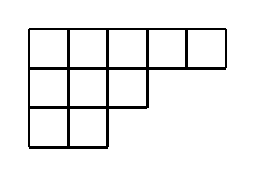
\begin{tikzpicture}[scale=0.5, line width=1pt]
  \draw (0,0) grid (5,1);
  \draw (0,0) grid (3,-1);
  \draw (0,-1) grid (2,-2);
\end{tikzpicture}
\end{center}

\begin{proposition}
For all positive integers $k \leq n$, the number of partitions of $n$ that have at least $k$ parts is equal to the number
of partitions of $n$ in which the largest part is at least $k$.
\end{proposition}

\begin{proposition}
For every positive integer $n$, the number of partitions of $n$ in which the first two parts are equal is equal to the number of partitions of $n$ 
in which each part is at least $2$.
\end{proposition}

\begin{lemma}
Let $m > k \geq 1$. Let $S$ be the set of partitions of $n$ into $m$ parts, the smallest of which is equal to $k$, and let $T$ be the set of partitions of 
$n$ into $m-1$ parts, in which the $k$th part is larger than the $(k+1)$st part and the smallest part is at least $k$.
Then $|S| = |T|$.
\end{lemma}

\subsubsection{Euler's totient function}\label{combinatoricstotient}

For any positive integer $n$, let $\phi(n)$ denote the number of positive integers $k \leq n$ that are relatively prime to $n$.

\begin{proposition}
Let $n = pq$, where $p$ and $q$ are distinct prinmes. Then $\phi(n) = (p-1)(q-1).$
\end{proposition}

\begin{proof}
Use the \hyperref[inclusionexclusion]{inclusion-exclusion principle} on $[pq]$, followed by the \hyperref[subtraction]{subtraction principle}.
\end{proof}

\begin{proof}
Let $n = p_1p_2\dots p_t$, where the $p_i$ are pairwise distinct primes. Then\dots
$$\phi(n) = \prod^t_{i=1}(p_i - 1).$$
\end{proof}

\begin{lemma}
Let $a$ and $b$ be two positive integers whose greates common divisor is $1$, and let $n = ab$. Then $\phi(n) = \phi(a)\phi(b).$
\end{lemma}

\begin{proposition}
For any prime $p$, and any positive integer $d$,
$$\phi(p^d) = (p-1)p^{d-1}.$$
\end{proposition}

\begin{proposition}
Let $n = p_1^{d_1}p_2^{d_2}\dots p_t^{d_t}$, where the $p_i$ are distinct primes. Then\dots
$$\phi(n) = \prod^t_{i=1}p_i^{d_i-1}(p_i - 1)$$
\end{proposition}


\subsection{Permutations}\label{permutation}
Given a set $A$, a \emph{permutation} of $A$ is a \hyperref[bijection]{bijection} $f : A \rightarrow A$.

\begin{proposition}\label{factorial}
Given a finite set $A$, if $n = |A|$ the number of permutations of $A$ is $n!$.
\end{proposition}

Intuitively permutations represent the reordering of an ordered list\label{list}. Looking at the idea of "sub-orderings" of lists we come up with the following proposition\dots

\begin{proposition}[k-lists]\label{k-list}
Let $n$ and $k$ be positive integers so that $n \geq k$. Then the number of injections $f : [k] \rightarrow [n]$ is\dots
$$(n)_k := n(n-1)(n-2)\cdots(n-k+1).$$
\end{proposition}

\subsection{Twelvefold Way}\label{twelvefoldway}

There are $12$ fundamental counting problems. Sometimes they are formulated in terms of putting \emph{balls} into \emph{baskets}.\newline

Let $N$ and $K$ be finite sets and $n$ and $k$ be their cardinality respectively\dots

\subsubsection{Functions from $K$ to $N$}

Count with sequences of $k$ elements in $N$, $|^KN|$.

\subsubsection{Injections from $K$ to $N$}

Count with \hyperref[k-list]{k-lists}, $(n)_k$.

\subsubsection{Surjections from $K$ to $N$}

Count with the number of sur

\subsubsection{Injections from $K$ to $N$, up to a permutation of $K$}

Count with 

\subsubsection{Functions from $K$ to $N$, up to a permutation of $K$}

Count with 

\subsubsection{Surjections from $K$ to $N$, up to a permutation of $K$}

Count with 

\subsubsection{Injections from $K$ to $N$, up to a permutation of $N$}

Count with 

\subsubsection{Surjections from $K$ to $N$, up to a permutation of $N$}

Count with 

\subsubsection{Functions from $K$ to $N$, up to a permutation of $N$}

Count with 

\subsubsection{Functions from $K$ to $N$, up to a permutation of $K$ and $N$}

Count with 

\subsubsection{Injections from $K$ to $N$, up to a permutation of $K$ and $N$}

Count with 

\subsubsection{Surjections from $K$ to $N$, up to a permutation of $K$ and $N$}

Count with 

\subsection{Graphs}\label{graph}
\newpage

\section{Category Theory}\label{categorytheory}

\subsection{Metacategories}\label{metacategory}

\subsubsection{Undefined notions}
\begin{itemize}
  \item \emph{Objects:} $a,b,c\dots$
  \item \emph{Arrows:} $f,g,h\dots$
\end{itemize}

\subsubsection{Operations}
Given $f: a \rightarrow b$\dots
\begin{itemize}
  \item \emph{Domain:} $\textbf{dom}\textrm{: arrows} \rightarrow \textrm{objects}$, $f \mapsto a$
  \item \emph{Codomain:} $\textbf{cod}\textrm{: arrows} \rightarrow \textrm{objects}$, $f \mapsto b$
  \item \emph{Identity:} $\textbf{id}\textrm{: objects} \rightarrow \textrm{arrows}$, $a \mapsto \textrm{id}_a = 1_a$
  \item \emph{Composition:} $\textbf{comp}\textrm{: arrows} \times \textrm{: arrows} \rightarrow \textrm{arrows}$, $\langle g, f \rangle \mapsto g \circ f$, \newline $g \circ f: \textrm{dom} f \rightarrow \textrm{cod} g$
\end{itemize}
\begin{figure}[!h]
\centering
\begin{tikzcd}
						  					 & b \arrow[dr, "g"] & \\
	a \arrow[rr, "g \circ f"] \arrow[ur, "f"] & 					 & c
\end{tikzcd}
\end{figure}

\subsubsection{Axioms}
\begin{itemize}
  \item \emph{Associativity:} $a \xrightarrow[]{f} b \xrightarrow[]{g} c \xrightarrow[]{k} d$, $k \circ (g \circ f) = (k \circ g) \circ f$
  \begin{figure}[!h]
  \centering
  \begin{tikzcd}[column sep=huge, row sep=huge]
	a \arrow[r, "k \circ (g \circ f) = (k \circ g) \circ f"] \arrow[d, "f" near start] \arrow[rd, "g \circ f" near end] & d \\
	b \arrow[r, "k \circ g"] \arrow[ru, "k \circ g" near start] & c \arrow[u, "k" near end]
\end{tikzcd}
  \end{figure}
  \item \emph{Unit Law:} $1_a \circ f = f$ and $g \circ 1_b = g$
  \begin{figure}[!h]
  \centering
  \begin{tikzcd}
	a \arrow[r,"f"] \arrow[rd, "f"] & b \arrow[d, "1_b"] \arrow[rd, "g"] & \\
	  & b \arrow[r, "g"] & c
\end{tikzcd}
  \end{figure}
\end{itemize}

\subsection{Categories}\label{category}

\subsubsection{Directed \hyperref[graph]{Graph}}\label{directedgraph}
\begin{itemize}
  \item $A$ - a set of arrows
  \item $O$ - a set of objects
  \item $\textbf{dom}: A \rightarrow O$, $\textbf{cod}: A \rightarrow O$
\end{itemize} 

\subsubsubsection{Set of composable pairs of arrows}\label{composablepairsofarrows}
$$A \times_O A = \{ \langle g, f \rangle | g, f \in A \textrm{ and } \textbf{dom} (g) = \textbf{cod} (f) \}$$

\subsubsection{Categories}\label{categorydefinition}
Add the following structure to a directed graph\dots
\begin{itemize}
  \item $O \xrightarrow[]{id} A$, $c \mapsto id_C$
  \item $A \times_O A \xrightarrow[]{\circ} A$, $\langle g, f \rangle \mapsto g \circ f$
\end{itemize}
which satisfy $\forall a \in O \textrm{ and } \forall \langle g, f \rangle \in A \times_O A$\dots
\begin{itemize}
  \item $\textbf{dom}(\textbf{id}(a)) = a = \textbf{cod}(\textbf{id}(a))$
  \item $\textbf{dom}(g \circ f) = \textbf{dom}(f)$
  \item $\textbf{cod}(g \circ f) = \textbf{cod}(g)$
  \item metacategorical axioms
\end{itemize}

\subsubsection{Small categories}\label{smallcategories}
\emph{Small categories} use \hyperref[smallsets]{small sets} for their objects.

\subsubsection{Hom Sets}\label{homset}
$hom(b,c) = \{f | f \in C, \textbf{dom}(f) = b, \textbf{cod}(f) = c \}$

\subsubsubsection{Alternate Definition of Categories}\label{homsetcategories}

Small categories may be defined with hom-sets as follows\dots
\begin{enumerate}
  \item A set of objects $a,b,c$\dots
  \item A function which assigns to each ordered pair $\langle a, b \rangle$ of objects a set hom$(a,b)$
  \item For each ordered triple $\langle a,b,c \rangle$ of objects a function
  			$$\textrm{hom}(b,c)\times\textrm{hom}(a,b) \rightarrow \textrm{hom}(a,c)$$
  		\mbox{called composition, and written $\langle g,f \rangle \rightarrow g \circ f$ for $g \in \textrm{hom}(b,c)$, $f \in \textrm{hom}(a,b)$}
  \item For each object $b$, an element $1_b \in \textrm{hom}(b,b)$, called the identity of $b$.
  \item If $\langle a,b \rangle \neq \langle a',b' \rangle$, then $\textrm{hom}(a,b) \cap \textrm{hom}(a',b') = \emptyset$
\end{enumerate}

\noindent The above satisfy the meta-categorical axioms.\newline

\hyperref[functors]{Functors} in terms of hom-sets are the object function with a collection of functions\label{homfunctors}
$$T_{c,c'}:\textrm{hom}_C(c,c') \rightarrow \textrm{hom}_B(Tc,Tc')$$
such that each $T_{c,c'}1_c = 1_{Tc}$ and every diagram\dots

\begin{figure}[H]
  \centering
  \begin{tikzcd}[column sep=huge, row sep=huge]
	hom_C(c',c'') \times hom_C(c,c') \arrow[r, "\circ"] \arrow[d, "T_{c',c''} \times T_{c,c'}"] & hom_C(c,c'') \arrow[d, "T_{c',c''}"] \\
	hom_B(Tc',Tc'') \times hom_B(Tc,Tc') \arrow[r, "\circ"]  									& hom_B(Tc,Tc'') 
\end{tikzcd}
\end{figure}

\noindent is commutative.

\subsubsection{Groupoids}\label{groupoid}
A category in which every arrow is an isomorphism.

\subsection{Morphisms}\label{morphism}
Arrows in categories.

\subsubsection{Isomorphisms}\label{isomorphism}
A morphism $f \in hom(b,c)$ that has a two-sided inverse $g \in hom(c,b)$ under composition such that
$$gf = 1_b, \textrm{ } fg = 1_c.$$

\begin{proposition}
The inverse of an isomorphism is unique.
\end{proposition}

\begin{proof}
For inverses $g_1,g_2$ of $f$ observe\dots
$$g_1 = g_11_c = g_1(fg_2) = (g_1f)g_2 = 1_bg_2 = g_2$$
\end{proof}

\begin{proposition}
Supposing $f^{-1}$ is the inverse of $f$\dots
\begin{itemize}
  \item Each identity $1_c$ is an isomorphism and is its own inverse.
  \item If $f$ is an isomorphism, then $f^{-1}$ is an isomorphism and further $(f^{-1})^{-1} = f$.
  \item If $f \in hom(a,b)$, $g \in hom(b,c)$ are isomorphisms, then the composition $gf$ is an isomorphism and $(gf)^{-1} = f^{-1}g^{-1}$. 
\end{itemize}
\end{proposition}

\subsubsection{Automorphisms}\label{automorphism}
An isomorphism of an object to itself. Denoted:
$$hom(c,c) = aut(c)$$
Observe $aut(c)$ is a group.

\subsubsection{Monomorphisms}\label{monomorphism}
A morphism $f \in hom(b,c)$ such that $\forall z \in C \textrm{ and } \forall \alpha',\alpha'' \in hom(z,b)$:
$$f\circ\alpha'=f\circ\alpha'' \Rightarrow \alpha'=\alpha''$$

\subsubsection{Epimorphisms}\label{epimorphism}
A morphism $f \in hom(b,c)$ such that $\forall z \in C \textrm{ and } \forall \beta',\beta'' \in hom(b,z)$:
$$\beta'\circ f = \beta''\circ f \Rightarrow \beta'=\beta''$$

\subsubsection{Split Morphism}\label{splitmorphism}
A morphism $f : b \rightarrow b$ such that $f^2 = f$ and there exist morphisms $g:b \rightarrow c$, $h: c \rightarrow b$ satisfying\dots
$$f=hg \; \; \land \; \; gh=1_c$$

\subsection{Some Objects in Categories}\label{someobjects}

\subsubsection{Initial Objects}\label{initial}

We say that an object $i$ of a category $C$ is \emph{initial} in $C$ if for every object $a$ of $C$ there exists exactly one morphism $i \rightarrow a$ in $C$:

$$\forall a \in Obj(C): \; \; Hom_C(i,a) \textrm{ is a singleton}.$$

\subsubsection{Final Objects}\label{final}

We say that an object $f$ of a category $C$ is \emph{final} in $C$ if for every object $a$ of $C$ there exists exactly one morphism $a \rightarrow f$ in $C$:

$$\forall a \in Obj(C): \; \; Hom_C(a,f) \textrm{ is a singleton}.$$

\begin{proposition}
Let $C$ be a category.
\begin{itemize}
  \item If $i_1$, $i_2$ are both initial objects in $C$, then $i_1 \cong i_2$.
  \item If $f_1$, $f_2$ are both initial objects in $C$, then $f_1 \cong f_2$.
\end{itemize}
\end{proposition}

\subsubsection{Null Objects}\label{null}

An object that is both initial and terminal.

\subsubsection{Group Objects}\label{groupobjects}

A \emph{group object} in $C$ consists of an object $g$ of $C$ and of morphisms\dots
$$m : g \times g \rightarrow g, \; e : 1 \rightarrow g, \; \iota : g \rightarrow g$$
in $C$ such that the diagrams\dots

\begin{figure}[H]
\centering

\begin{tikzcd}[column sep=huge, row sep=huge]
	(g \times g) \times g \arrow[r, "m \times \textrm{id}_g"] \arrow[d] & g \times g \arrow[r, "m"] & g \arrow[d, "="]\\
	g \times (g \times g) \arrow[r, "\textrm{id}_g \times m"] & g \times g \arrow[r, "m"] & g
\end{tikzcd}

\end{figure}

\begin{figure}[H]
\centering

\[ \begin{array}{cc}
\begin{tikzcd}[column sep=huge, row sep=huge]
	1 \times g \arrow[r, "e \times \textrm{id}_g"] \arrow[rd, "\cong" below] & g \times g \arrow[d, "m"]\\
	 & g
\end{tikzcd}

&

\begin{tikzcd}[column sep=huge, row sep=huge]
	g \times 1 \arrow[r, "\textrm{id}_g \times e"] \arrow[rd, "\cong" below] & g \times g \arrow[d, "m"]\\
	 & g
\end{tikzcd}
\end{array} \]

\end{figure}

\begin{figure}[H]
\centering

\[ \begin{array}{cc}
\begin{tikzcd}[column sep=huge, row sep=huge]
	g \arrow[r, "\Delta"] \arrow[d] & g \times g \arrow[r, "\textrm{id}_g \times \iota"] & g \times g \arrow[d, "m"]\\
	1 \arrow[rr, "e"] & & g
\end{tikzcd}

&

\begin{tikzcd}[column sep=huge, row sep=huge]
	g \arrow[r, "\Delta"] \arrow[d] & g \times g \arrow[r, "\iota \times \textrm{id}_g"] & g \times g \arrow[d, "m"]\\
	1 \arrow[rr, "e"] & & g
\end{tikzcd}
\end{array} \]

\end{figure}

commute.

\subsubsubsection{Group Action}\label{categoricalgroupactions}

If $G$ is a group and $a$ an object of a category $C$, then a \emph{group action} is a functor\dots
$$\sigma : G \rightarrow \textrm{Aut}_C(a)$$

\subsection{Functors}\label{functor}
Morphisms $T: C \rightarrow B$ with domain and codomain both categories. It consists of two suitably related functions
\begin{itemize}
  \item object function $T$, $c \mapsto Tc$
  \item arrow function $T$, $f:c \rightarrow c' \mapsto Tf:Tc \rightarrow Tc'$
\end{itemize}
which satisfy\dots
\begin{itemize}
  \item $T(1_c) = 1_c$
  \item $T(g \circ f) = T_g \circ T_f$
\end{itemize}

\subsubsection{Full}\label{full}
$\forall c, c' \in C \textrm{ and } g:Tc \rightarrow Tc' \in B, \exists f:c \rightarrow c' \in C \textrm{ s.t. } g \in Tf$

\subsubsection{Faithful}\label{faithful}
$\forall c, c' \in C \textrm { and } f_1,f_2:c \rightarrow c', Tf_1 = Tf_2 \Rightarrow f_1=f_2$

\subsubsection{Forgetful}\label{forgetful}
A functor that drops some of the structure of its input. For example, the forgetful functor $U: \textrm{Cat} \rightarrow \textrm{Graph}$\dots
\begin{itemize}
  \item $C \mapsto UC$ where $UC$ is comprised of the underlying objects and arrows of the category
  \item $F:C \rightarrow C' \mapsto UF:UC \rightarrow UC'$ where $UF$ is a \hyperref[graphisomorphisms]{morphism} between corresponding graphs
\end{itemize}

\subsection{Natural Transformations}\label{naturaltransformations}

Given two functors $S,T: C \rightarrow B$ a \emph{natural transformation} $\tau : S \xrightarrow[]{\cdot} T$ is a function which assigns to each object $c \in C$ an arrow
$$\tau_c = \tau c: Sc \rightarrow Tc$$
of $B$ in such a way that every arrow $f: c \rightarrow c'$ in $C$ yields a diagram\dots\newline

\begin{figure}[H]
\centering

\[ \begin{array}{cc}
\begin{tikzcd}
	c \arrow[d, "f"]\\
	c'
\end{tikzcd}

&

\begin{tikzcd}
	Sc \arrow[r, "\tau c"] \arrow[d, "Sf"] & Tc \arrow[d, "Tf"]\\
	Sc' \arrow[r, "\tau c'"]				 & Tc'
\end{tikzcd}
\end{array} \]

\end{figure}

\noindent which is commutative. \newline

\noindent In the following diagram $\tau a, \tau b, \tau c$ are the components of the natural transformation.

\begin{figure}[H]
\centering

\[ \begin{array}{cc}
\begin{tikzcd}
	a \arrow[dr, "f"] \arrow[dd, "h"] &   \\
					  				  & c \\
	b \arrow[ur, "g"] 				  &
\end{tikzcd}

&

\begin{tikzcd}
	Sa \arrow[dr, "Sf"] \arrow[dd, "Sh"] \arrow[rr, "\tau a"] &    								   & Ta \arrow[dr, "Tf"] \arrow[dd, "Th" near start] &    \\
					  				     					  & Sc \arrow[rr, "\tau c" near start] & 									   			 & Tc \\
	Sb \arrow[ur, "Sg"] \arrow[rr, "\tau b"]				  &	  								   & Tb \arrow[ur, "Tg"] 				   			 &
\end{tikzcd}
\end{array} \]

\end{figure}

\subsection{Duality}\label{duality}

\begin{center}
\begin{tabular}{ll}
Statement $\sum$ & Dual Statement $\sum^*$\\
\hline
$f: a \rightarrow b$ & $f: b \rightarrow a$\\
$a = \textrm{dom} f$ & $a = \textrm{cod} f$\\
$i=1_a$ & $i=1_a$\\
$h = g \circ f$ & $h = f \circ g$\\
$f$ is a monomorphism & $f$ is an epimorphism\\
$u$ is a right inverse of $h$ & $u$ is a left inverse of $h$\\
$f$ is invertible & $f$ is invertible\\
$f$ is a terminal object & $f$ is an initial object
\end{tabular}
\end{center}

\subsection{Contravariance and Opposites}\label{contravariance}

\subsubsection{Contravariant Functor}\label{contravariantfunctor}
Given a functor $S: C^{op} \rightarrow B$ the \emph{contravariant functor} $\overline{S} : C \rightarrow B$ satisfies\dots
\begin{itemize}
  \item $\overline{S}f = Sf^{op}$,
  \item $c \mapsto \overline{S}c$,
  \item $f:a \rightarrow b \mapsto \overline{S}f:\overline{S}b \rightarrow \overline{S}a$,
  \item $\overline{S}(1_c) = 1_{\overline{S}c}$,
  \item $\overline{S}(fg) = (\overline{S}g)(\overline{S}f)$.
\end{itemize}

\subsubsubsection{Covariant Hom-Functor}\label{covarianthomfunctor}
A \hyperref[homfunctors]{hom-functor} $C(a,-) = hom(a,-):C \rightarrow \textrm{Set}$ satisfying\dots
\begin{itemize}
  \item $b \mapsto hom(a,b)$
  \item $k:b\rightarrow b' \mapsto hom(a,k):hom(a,b) \rightarrow hom(a,b')$; the right side maps $f \mapsto k \circ f$ and is denoted $k*$
\end{itemize}

\subsubsubsection{Contravariant Hom-Functor}\label{contravarianthomfunctor}
A \hyperref[homfunctors]{hom-functor} $C(-,b) = hom(-,b):C^{op} \rightarrow \textrm{Set}$ satisfying\dots
\begin{itemize}
  \item $a \mapsto hom(a,b)$
  \item $g:a\rightarrow a' \mapsto hom(g,a):hom(a',b) \rightarrow hom(a,b)$; the right side maps $f \mapsto f \circ g$ and is denoted $g*$
\end{itemize}

\noindent The functions $g^*, k^*$ defined above satify the following commutative diagram.

\begin{figure}[H]
  \centering
  \begin{tikzcd}[column sep=huge, row sep=huge]
	hom(a',b)  \arrow[r, "g*"] \arrow[d, "k*"] & hom(a,b) \arrow[d, "k*"] \\
	hom(a',b') \arrow[r, "g*"]  			   & hom(a,b') 
\end{tikzcd}
\end{figure}

\subsection{Category Constructions}\label{categoryconstructions}

\subsubsection{Products}\label{products}

Given categories $B$ and $C$ we construct the product category $B \times C$\dots
\begin{itemize}
  \item Objects: pairs of objects $\langle b,c \rangle$ ($b \in B$ and $c \in C$)
  \item Arrows: $\langle b,c \rangle \rightarrow \langle b',c' \rangle$ are a pair $\langle f,g \rangle$ of arrows ($f \in B$ and $g \in C$)
  \item Composition: $\langle f', g' \rangle \circ \langle f, g \rangle = \langle f' \circ f, g' \circ g \rangle$
\end{itemize}

\noindent The corresponding \hyperref[universality]{universal property} is: for any functors $R$ and $T$, there is a unique functor $F$ making the digram commute\dots

\begin{figure}[H]
\centering
\begin{tikzcd}
	& D \arrow[ld,"R" above] \arrow[d, dotted, "F"] \arrow[rd,"T"]& \\
	B  & B \times C \arrow[r, "Q" below] \arrow[l, "P"] & C
\end{tikzcd}
\end{figure}

\noindent Note: $P\langle f,g \rangle = f$ and $Q\langle f,g \rangle = g$ are called the \emph{projections}\label{projections} of the product.

\subsubsubsection{Products of Functors}\label{functorproducts}
Given functors $U$ and $V$, the functor product $U \times V$ satisfies\dots
\begin{itemize}
  \item $(U \times V)\langle b,c \rangle = \langle Ub,Uc \rangle$ for objects
  \item $(U \times V)\langle f,g \rangle = \langle Uf,Ug \rangle$ for arrows
\end{itemize}

\begin{figure}[H]
\centering
\begin{tikzcd}[column sep=huge, row sep=huge]
	B  \arrow[d, "U"] & B \times C \arrow[l, "P" above] \arrow[r, "Q"] \arrow[d, dotted, "U \times V"] & C \arrow[d, "V"]\\
	B 				  & B \times C \arrow[l, "P'" above] \arrow[r, "Q'"]							   & B
\end{tikzcd}
\end{figure}

\subsubsubsection{Bifunctors}\label{bifunctors}

A functor $S : B \times C \rightarrow D$. Intuitively, "a functor of two variables."\newline

\noindent Determined by the functors that result when any one object of exactly one of the categories is fixed. This is
recorded more explicitly in the following proposition\dots

\begin{proposition}
Let $B,C$, and $D$ be categories. For all objects $c \in C$ and $b \in B$, let
$$L_c : B \rightarrow D, \; M_b : C \rightarrow D$$
be functors such that $M_b(c) = L_c(b)$ for all $b$ and $c$. Then there exists a bifunctor $S: B \times C \rightarrow D$
with $S(-, c) = L_c$ for all $c$ and $S(b,-) = M_b$ for all $b$ if and only if for every pair of arrows $f:b \rightarrow b'$
and $g:c \rightarrow c'$ one has
$$M_{b'}g \circ L_cf = L_{c'}f \circ M_bg.$$
These equal arrows in $D$ are then the value $S(f,g)$ of the arrow function of $S$ at $f$ and $g$.
\end{proposition}

\begin{proof}
Observe\dots
$$\langle b',g \rangle \circ \langle f,c \rangle  = \langle b'f,gc \rangle = \langle f,g \rangle =  \langle fb,c'g \rangle = \langle f,c' \rangle \circ \langle b,g \rangle$$
(where $b,b',c,c'$ are identity arrows).\newline

\noindent This implies\dots
$$S(b',g)S(f,c)=S(f,c')S(b,g).$$
Which further implies\dots

\begin{figure}[H]
\centering
\begin{tikzcd}[column sep=huge, row sep=huge]
	S(b,c) \arrow[d, "S(f\textrm{,}c)"] \arrow[r, "S(b\textrm{,}g)"] & S(b,c') \arrow[d, "S(f\textrm{,}c')"] \\
	S(b',c) \arrow[r, "S(b'\textrm{,}g)"] & S(b',c') 
\end{tikzcd}
\end{figure}

\end{proof}

\subsubsubsection{Natural transformations between bifunctors}
Given $S,S':B \times C \rightarrow D$. Consider $\alpha(b,c) : S(b,c) \rightarrow S'(b,c)$. We say $\alpha$ is \emph{natural in}\label{naturalin} $b$ if $\forall c \in C$ the components $\alpha(b,c)$
for all $b$ define $\alpha(-,c): S(-,c) \xrightarrow[]{\cdot} S'(-,c)$, a natural transformation of functors $B \rightarrow D$.

\begin{proposition}
For bifunctors $S,S'$, the function $\alpha$ displayed above is a natural transformation $\alpha:S \xrightarrow[]{\cdot} S'$ (i.e., of bifunctors) if and only if $\alpha(b,c)$ is natural
in $b$ for each $c \in C$ and natural in $c$ for each $b \in B$.

\begin{figure}[H]
\centering
\begin{tikzcd}[column sep=huge, row sep=huge]
	S(b,c) \arrow[d, "S(f\textrm{,}g)"] \arrow[r, "\alpha(f\textrm{,}g)"] & S(b,c) \arrow[d, "S'(b\textrm{,}c)"] \\
	S(b',c') \arrow[r, "\alpha(b'\textrm{,}c')"] & S(b',c') 
\end{tikzcd}
\end{figure}

\end{proposition}

\subsubsubsection{The Universal Natural Transformation}\label{universalnaturaltransformation}

Given any natural transformation $\tau: S \xrightarrow[]{\cdot} T$ between $S,T: C \rightarrow B$ there is a unique functor $F: C \times 2 \rightarrow B$ with $F \mu c = \tau c$ for any object $c$.
\begin{itemize}
  \item $F\langle f,0 \rangle = Sf$
  \item $F\langle f,1 \rangle = Tf$
  \item $F\langle f, \downarrow \rangle = Tf \circ \tau c = \tau c' \circ Sf$ (where $\downarrow : 0 \rightarrow 1$)
\end{itemize}

\noindent Observe $C \times 2$ below\dots

\begin{figure}[H]
\centering
\begin{tikzcd}
	c \arrow[dr] \arrow[dd, "C \times 0 \textrm{ layer}" description ] \arrow[rr, "\mu c"] &    								   & c \arrow[dr, "C \times 1 \textrm{ layer}" description, near end ] \arrow[dd] &    \\
					  				     		 & c'' \arrow[rr, "\mu c''" near start] & 					     & c'' \\
	c' \arrow[ur] \arrow[rr, "\mu c'"]		     &	  								   & c' \arrow[ur] 			 &
\end{tikzcd}
\end{figure}

\noindent where $\mu c = \langle c, \downarrow \rangle$

\subsubsection{Coproducts}\label{products}

Given categories $B$ and $C$ the dual of the product category is coproduct category $B \coprod C$.\newline

\noindent The corresponding \hyperref[universality]{universal property} is: for any functors $R$ and $T$, there is a unique functor $F$ making the digram commute\dots
\begin{figure}[H]
\centering
\begin{tikzcd}
	B \arrow[r, "I" above] & B \coprod C & C \arrow[l, "J" above]\\
	& D \arrow[lu,"R" below] \arrow[u, dotted, "F"] \arrow[ru,"T" below] &
\end{tikzcd}
\end{figure}

\subsubsection{Quotients}\label{quotients}

The \emph{quotient category} is specified in the following proposition.

\begin{proposition}
For a given category $C$, let $R$ be a function which assigns to each pair of objects $a,b$ of $C$ a binary relation $R_{a,b}$ on the hom-set $C(a,b)$.
Then there exist a category $C/R$ and a functor $Q = Q_R:C \rightarrow C/R$ such that\dots
\begin{enumerate}
  \item If $fR_{a,b}f'$ in $C$, then $Qf = Qf'$.
  \item If $H:C \rightarrow D$ is any functor from $C$ for which $f R_{a,b} f'$ implies $Hf = Hf'$ for all $f$ and $f'$, then there is a unique functor $H':C/R \rightarrow D$
  with $H' \circ Q_R = H$.
\end{enumerate}
Moreover, the functor $Q_R$ is a bijection on objects.
\end{proposition}

\noindent The corresponding \hyperref[universality]{universal property} is represented in the following diagram\dots

\begin{figure}[H]
\centering

\begin{tikzcd}
	C \arrow[r, "Q_R"] \arrow[dr, "H" below] & C/R \arrow[d, dotted, "H'"]\\
								 		   & D
\end{tikzcd}

\end{figure}

\subsubsubsection{Congruence}\label{congruence}
A \emph{congruence} is a relation $R$ on a category $C$ such that\dots
\begin{itemize}
  \item $\forall a,b \in \text{Obj}(C)$, $R_{a,b}$ is an \hyperref[equivalencerelation]{equivalence relation}
  \item if $f,f':a \rightarrow b$ have $f R_{a,b} f'$, then for all $g: a' \rightarrow a$ and all $h: b \rightarrow b'$ one has $(hfg)R_{a',b'}(hf'g)$.
\end{itemize}

\subsubsection{Free Categories}\label{freecategories}

\subsubsubsection{O-graph}\label{ograph}
The \emph{O-graph} is a graph on a fixed set $O$ of objects such that $O$-graph morphisms $D_O$ are always equal to $id_O$.\newline

\noindent We define the \emph{product over O} as a \hyperref[composablepairsofarrows]{set of composable pairs of arrows}\dots
$$A \times_O B = \{ \langle g, f \rangle | \delta_0 g = \delta_1 f, g \in A, f \in B \}$$

\noindent A \hyperref[category]{category} with objects $O$ is an $O$-graph equipped with two morphisms $c:A \times_O A \rightarrow A$ and $i:O \rightarrow A$
of $O$-graphs making the following diagrams commutative.

\[ \begin{array}{cc}

\begin{tikzcd}[column sep=small]
	(A \times_O A) \times_O A \arrow[d,"c \times 1"] \arrow[r,"\cong"] & A \times_O (A \times_O A) \arrow[r,"1 \times c"] & A \times_O A \arrow[d,"c"]\\
	A \times_O A \arrow[rr,"c"] & & A
\end{tikzcd}

&

\begin{tikzcd}
	O \times_O A \arrow[r,"i \times 1"] \arrow[d,"\cong"] & A \times_O A \arrow[d,"c"] & A \times_O O \arrow[l,"1 \times i" above] \arrow[d,"\cong"]\\
	A \arrow[r,"="] & A & A \arrow[l,"="]
\end{tikzcd}

\end{array} \]


\subsubsubsection{Free Category}\label{freecategory}

Let $C(G)$ be the \emph{free category} generated by graph $G$, specified in the subsequent theorem\dots

\begin{theorem}
Let $G = \{A \rightrightarrows O\}$ be a small graph. There is a small category $C(G)$ with $O$ as its set of objects and a morphism $P: G \rightarrow UC$ of graphs from $G$ to
the underlying graph $UC$ of $C$ with the following property. Given any category $B$ and any morphism $D:G \rightarrow UB$ of graphs, there is a unique functor $D':C \rightarrow B$
with $(UD') \circ P = D$, as in the commutative diagram

\noindent The corresponding \hyperref[universality]{universal property} is: for any functors $R$ and $T$, there is a unique functor $F$ making the digram commute\dots
\begin{figure}[H]
\centering
\begin{figure}[H]
\centering

\[ \begin{array}{cc}
\begin{tikzcd}
	C \arrow[d, dotted, "D'"]\\
	B
\end{tikzcd}

&

\begin{tikzcd}
	G \arrow[r, "P"] \arrow[dr, "D" below] & UC \arrow[d, dotted, "UD'"]\\
								 		   & UB
\end{tikzcd}
\end{array} \]

\end{figure}
\end{figure}

In particular, if $B$ had $O$ as set of objects and $D$ is a morphism of $O$-graphs, then $D'$ is the identity on objects.
\end{theorem}

\begin{corollary}
To any set $X$ there is a monoid $M$ and a function $p: X \rightarrow UM$, where $UM$ is the underlying set of $M$, with the following universal property: for any monoid $L$ and any
function $h: X \rightarrow UL$ there is a unique morphism $h': M \rightarrow L$ of monoids with $h: Uh' \circ p$.
$$\textrm{Hom}_{Cat}(C(G),B) \cong \textrm{Grph}(G,UB), \; D' \mapsto D = UD' \circ P$$
\end{corollary}

\subsubsection{Comma Categories}\label{commacategories}

\subsection{Higher Level Categories}\label{higherlevelcategories}

\subsubsection{Functor Categories}\label{functorcategories}

A \emph{functor category} is a category whose objects are \hyperref[functor]{functors} and whose arrows are \hyperref[naturaltransformations]{natural transformations}.
Since compositions of natural transformations are natural transformations, composition can be defined as in the following diagram\dots

\begin{figure}[H]
  \centering
  \begin{tikzcd}[column sep=huge, row sep=huge]
	Rc \arrow[r, "Rf"] \arrow[d, "\sigma c"] \arrow[dd, bend right, "(\tau \circ \sigma)c" left] & Rc' \arrow[d, "\sigma c'" left] \arrow[dd, bend left, "(\tau \circ \sigma)c'"] \\
	Sc \arrow[r, "Sf"] \arrow[d, "\tau c"]   													 & Sc' \arrow[d, "\tau c'" left] \\
	Tc \arrow[r, "Tf"] 						 													 & Tc'
\end{tikzcd}
\end{figure}

\subsubsection{2-Categories}

\subsubsubsection{Vertical Composition}\label{verticalcomposition}
For natural transformations $\tau$ and $\sigma$, we have "vertical" composition $\tau \dot \sigma$, as in the following diagram\dots

\begin{figure}[H]
  \centering
  \begin{tikzcd}[column sep=huge, row sep=huge]
	C \arrow[r] \arrow[d, "\sigma"] \arrow[dd, bend right, "\tau\sigma" left] & B \arrow[d, "\sigma"] \arrow[dd, bend left, "\tau\sigma" right] \\
	C \arrow[r] \arrow[d, "\tau"]  											  & B \arrow[d, "\tau"] 											\\
	C \arrow[r] 											 				  & B
\end{tikzcd}
\end{figure}

\subsubsubsection{Horizontal Composition}\label{horizontalcomposition}
We can also define "horizontal" composition for natural transformations $\tau$ and $\tau'$, $\tau' \circ \tau$, as in the following commutative diagrams\dots

\begin{figure}[H]
  \centering
  \begin{tikzcd}[column sep=huge, row sep=huge]
	C \arrow[r, "S"] \arrow[d, "\tau"] & B \arrow[r, "S'"] \arrow[d, bend right, "\tau" left] \arrow[d, bend left, "\tau'"] & A \arrow[d, "\tau'"]\\
	C \arrow[r, "T"] & B \arrow[r, "T'"] & A
\end{tikzcd}
\end{figure}

\begin{figure}[H]
  \centering
  \begin{tikzcd}[column sep=huge, row sep=huge]
	S'Sc \arrow[r, "\tau'Sc"] \arrow[d, "S'\tau c"] \arrow[rd, dotted, "(\tau' \circ \tau)c"] & T'Sc \arrow[d, "T'\tau c"] \\
	S'Tc \arrow[r, "\tau'Tc"]				   	  									  & T'Tc 
\end{tikzcd}
\end{figure}

\noindent The next diagram shows $\tau' \circ \tau : S'S \xrightarrow[]{\cdot} T'T$ is natural.

\begin{figure}[H]
  \centering
  \[ \begin{array}{cc}

\begin{tikzcd}[column sep=huge, row sep=huge]
	c \arrow[d, "f"]\\
	b
\end{tikzcd}

&

\begin{tikzcd}[column sep=huge, row sep=huge]
	S'Sc \arrow[r, "S'\tau c"] \arrow[d, "S'S f"] & S'Tc \arrow[r, "\tau' Tc"] \arrow[d, "S'T f"] & T'Tc \arrow[d, "T'T f"] \\
	S'Sb \arrow[r, "T'\tau b"] & S'Tb \arrow[r, "\tau' Tb"] & T'Tb
\end{tikzcd}

\end{array} \]
\end{figure}

\noindent So $\tau' \circ \tau = (T' \circ \tau) \cdot (\tau' \circ S) = (\tau' \circ T) \cdot (S' \circ \tau)$, which leads into our next concept.

\subsubsubsection{Interchange Law}\label{interchangelaw}
For natural transformations $\sigma,\sigma',\tau,\tau'$ satisfying\dots

\begin{figure}[H]
  \centering
  \begin{tikzcd}[column sep=huge, row sep=huge]
	C \arrow[r] \arrow[d, "\sigma"] & B \arrow[r] \arrow[d, bend right, "\sigma" left] \arrow[d, bend left, "\sigma'"] & A \arrow[d, "\sigma'"] \\
	C \arrow[r] \arrow[d, "\tau"] & B \arrow[r] \arrow[d, bend right, "\tau" left] \arrow[d, bend left, "\tau'"] & A \arrow[d, "\tau'"] \\
	C \arrow[r] & B \arrow[r] & A
\end{tikzcd}
\end{figure}

\noindent the \emph{interchange law} is $(\tau' \cdot \sigma') \circ (\tau \cdot \sigma)=(\tau' \circ \tau)\cdot(\sigma' \circ \sigma).$ \newline

\noindent The proof of the interchange law derives from the following diagram. Intuitively, the interchange law occurs along the dotted diagonal lines.

\begin{figure}[H]
  \centering
  \begin{tikzcd}[column sep=huge, row sep=huge]
	S'Sc \arrow[r, "\sigma'S"] \arrow[d, "S'\sigma"] \arrow[rd, dotted] \arrow[rdrd, dotted, bend left] & T'Sc \arrow[r, "\tau'S"] \arrow[d, "T'\sigma"] 				   & R'Sc \arrow[d, "R'\sigma'"] \\
	S'Tc \arrow[r, "\sigma'T"] \arrow[d, "S'\tau"]  				    & T'Tc \arrow[r, "\tau'T"] \arrow[d, "T'\tau"] \arrow[rd, dotted]  & R'Tc \arrow[d, "R'\tau'"]   \\
	S'Rc \arrow[r, "\sigma'R"] 					   	 				 	& T'Rc \arrow[r, "\tau'R"] 					  					   & R'Rc
\end{tikzcd}
\end{figure}

\begin{theorem}
The collection of natural transformations in the set of arrows of two different categories under two different operations of composition, $\cdot$ and $\circ$, which satisfy the interchange
law. Moreover, any arrow (transformation) which is an identity for the composition $\circ$ is also an identity for the composition $\cdot$.
\end{theorem}

\subsubsubsection{Double Category}\label{doublecategory}
The set of arrows for two different compositions with two different compositions which together satisfy the interchange law.

\subsubsubsection{2-Category}\label{twocategories}
A double category in which every identiy arrow for the first composition is also an identity for the second composition.

\subsection{Universal Properties}\label{universality}
\newpage

\section{Category Examples}\label{examplecategories}

\subsection{The category Grp}
\begin{itemize}
  \item Objects: Groups
  \item Arrows: Homomorphisms
\end{itemize}

\begin{proposition}
Trivial groups are \hyperref[null]{null} objects in Grp.
\end{proposition}

\begin{proposition}
Grp has \hyperref[products]{products}. (See \hyperref[groupproduct]{Group Products})
\end{proposition}

\begin{proposition}
Grp has \hyperref[coproducts]{coproducts}. (See \hyperref[freegroupproduct]{Free Group Products})
\end{proposition}

\subsection{The category Ab}
\begin{itemize}
  \item Objects: Abelian Groups
  \item Arrows: Homomorphisms
\end{itemize}

\subsubsection{Morphisms}

\begin{proposition}
The following are equivalent:
\begin{enumerate}
  \item $\varphi$ is an epimorphism
  \item coker$\varphi = \{ e_{G'} \}$
  \item $\varphi : G \rightarrow G'$ is surjective (as a set function)
\end{enumerate}
\end{proposition}

\begin{proof}
$(1) \Rightarrow (2)$: Assume $(1)$ holds, and consider the two parallel compositions\dots
$$G \xrightarrow[]{\varphi} G' \underset{e}{\overset{\pi}{\rightrightarrows}} \textrm{coker} \varphi$$
where $\pi$ is the canonical projection and $e$ is the trivial map. Both $\pi \circ \varphi$ and $e \circ \varphi$ are the trivial map; since $\varphi$ is an epimorphism,
this implies $\pi = e$. But $\pi = e$ implies that coker$\varphi$ is trivial.

\noindent $(2) \Rightarrow (3)$: If coker$\varphi = G' / \textrm{im}\varphi$ is trivial, then im$\varphi = G'$; hence $\varphi$ is surjective.

\noindent $(3) \Rightarrow (1)$: If $\varphi$ is surjective, then it satisfies the universal property for epimorphisms in Set: for any set $Z$ and any two set-functions $\alpha'$ and
$\alpha'' : G' \rightarrow Z$,
$$\alpha' \circ \varphi = \alpha'' \circ \varphi \Leftrightarrow \alpha' = \alpha''.$$
This must hold in particular if $Z$ is endowed with a group structure and $\alpha',\alpha''$ are group homomorphisms, so $\varphi$ is an epimorphism in Grp.
\end{proof}

\subsubsection{Universal Objects}

\begin{proposition}
Trivial groups are \hyperref[null]{null} objects in Ab.
\end{proposition}

\begin{proposition}
Ab has \hyperref[products]{products} and \hyperref[coproducts]{coproducts}. They are the same
construct and are called \emph{Direct Sums}, denoted $G \oplus H$. (See \hyperref[groupproduct]{Group Products})
\end{proposition}
\newpage

\section{Group Theory}\label{grouptheory}

\subsection{Definition}\label{groupdefinition}

A \emph{group} is a \hyperref[groupoid]{groupoid} with a single object.\newline

\noindent A \emph{group} $\langle G, \LargerCdot \rangle$ is a set $G$ endowed with the binary operation $\LargerCdot$ such that\dots
\begin{enumerate}
  \item the operation $\cdot$ is \emph{associative}
  \item there exists an \emph{identity element} $e_G$ for $\LargerCdot$
  \item every element in $G$ has an \emph{inverse} with respect to $\LargerCdot$
\end{enumerate}

\noindent We can repeated elements as follows\dots
\begin{itemize}
  \item $g^n = g \LargerCdot g \cdots g \LargerCdot g$ ($n$ times)
  \item $g^{-n} = g^{-1} \LargerCdot g^{-1} \cdots g^{-1} \LargerCdot g^{-1}$ ($n$ times)
\end{itemize} 

\begin{proposition}
The identity $e_G \in G$ of a group is unique.
\end{proposition}

\begin{proof}
If $h$ is another identity, then $h = e_Gh = e_G$.
\end{proof}

\begin{proposition}
Inverses in a group $G$ are unique.
\end{proposition}

\begin{proposition}[Cancellation]\label{cancellation}
Let $G$ be a group. Then $\forall a,g,h \in G$\dots
$$ga = ha \Rightarrow g = h, \; \; ag = ah \Rightarrow g = h.$$
\end{proposition}

\subsection{Order}

\subsubsection{Order of an element}\label{elementorder}
The \emph{order of an element} $g \in G$, denoted $|g|$, is the smallers positive integer $n$ such that $g^n = e$.

\noindent $g$ has \emph{finite order} if any such integer exists.\newline

\noindent $g$ has \emph{infinite order} if no such integer exists, denoted $|g| = \infty$.\newline

\begin{lemma}
If $g^n = e$ for some positive integer $n$, then $|g|$ is a divisor of $n$.
\end{lemma}

\begin{proof}
As observed, $n \geq |g|$ for $n \in \mathbb{Z}$, that is $n - |g| \geq 0$. Since $\mathbb{Z}$ is a Euclidean domain, there must exist
an integer $m > 0$ such that\dots
$$r = n -|g|\cdot m \geq 0 \; \textrm{ and } \; n - |g| \cdot (m + 1) < 0,$$
that is, $r < |g|$. Note that\dots
$$g^r = g^{n - |g| \cdot m} = g^n \cdot (g^{|g|})^{-m} = e \cdot e^{-m} = e.$$
By definition of order, $|g|$ is the smallest positive integer such that $g^{|g|}=e.$ Since $r$ is smaller than $|g|$ and $g^r = e,$ $r$ cannot
be positive; hence $r = 0$ necessarily. So $n = |g| \cdot m$.
\end{proof}

\begin{corollary}
Let $g$ be an element of finite order, and let $N \in \mathbb{Z}$. Then
$$g^N = e \Leftrightarrow N \textrm{ is a multiple of } |g|$$
\end{corollary}

\subsubsection{Order of an group}\label{grouporder}
If $G$ is finite as a set, its \emph{order} $|G|$ is the number of its elements; we write $|G| = \infty$ if $G$ is infinite.

\begin{proposition}
Let $g \in G$ be an element of finite order. Then $g^m$ has finite order $\forall m \geq 0$, and in fact
$$|g^m| = \frac{\textrm{lcm}(m,|g|)}{m} = \frac{|g|}{\textrm{gcd}(m,|g|)}.$$
\end{proposition}

\begin{proof}
The order of $g^m$ is the least positive $d$ for which\dots
$$g^{md} = e.$$
In other words, $m|g^m|$ is the smallest multiple of $m$ which is also a multiple of $|g|$:
$$m|g^m| = \textrm{lcm}(m,|g|).$$
\end{proof}

\begin{proposition}
If $gh$ = $hg$, then $|gh|$ divides lcm$(|g|,|h|)$.
\end{proposition}

\begin{proof}
Observe\dots
$$(gh)^{\textrm{lcm}(m,n)} = (gh)(gh)\cdots(gh) = gg\cdots g \LargerCdot hh\cdots h = g^{\textrm{lcm}(m,n)}h^{\textrm{lcm}(m,n)} = e.$$
\end{proof}

\subsection{Homomorphism}\label{grouphomomorphism}

For groups $\langle G, \LargerCdot_G \rangle$, $\langle H, \LargerCdot_H \rangle$, a \emph{group homomorphism}\dots
$$\varphi : \langle G, \LargerCdot_G \rangle \rightarrow \langle H, \LargerCdot_H \rangle$$
is a \hyperref[function]{set-function} preserving the binary operations of the groups, i.e. the following diagram commutes\dots

\begin{figure}[H]
\centering
\begin{tikzcd}
G \times G \arrow[r, "\varphi \times \varphi"] \arrow[d, "\LargerCdot_G"] & H \times H \arrow[d, "\LargerCdot_H"]\\
G \arrow[r, "\varphi"] & H
\end{tikzcd}
\end{figure}

\noindent i.e. $\forall a,b \in G \textrm{ we have } \varphi(a \LargerCdot_G b) = \varphi(a) \LargerCdot_H \varphi(b)$.

\begin{proposition}
Let $\varphi : G \rightarrow H$ be a group homomorphism. Then\dots
\begin{itemize}
  \item $\varphi(e_G) = e_H$
  \item $\forall g \in G, \varphi (g^{-1}) = \varphi(g)^{-1}$.
\end{itemize}
\end{proposition}

\begin{proof}
For the first item observe\dots
$$e_H \dots \varphi(e_G) = \varphi(e_G) = \varphi(e_G \LargerCdot e_G) = \varphi(e_G) \LargerCdot \varphi(e_G) \Rightarrow e_H = \varphi(e_G).$$
For the second item observe\dots
$$\varphi (g^{-1}) \LargerCdot \varphi (g) = \varphi (g^{-1} \LargerCdot g) = \varphi (e_G) = e_H = \varphi (g)^{-1} \LargerCdot \varphi (g) \Rightarrow \varphi (g^{-1}) = \varphi (g)^{-1}$$
\end{proof}

\subsubsection{Some Important Morphisms}

\subsubsubsection{Trivial Morphism}\label{trivialmorphism}
Because $\{ * \}$ is a \hyperref[null]{null object} in Grp (and Ab) we are guaranteed unique morphisms\dots
$$\varphi : G \rightarrow \{ * \}, \; \psi : \{ * \} \rightarrow H.$$
We call the resulting composition $\psi \circ \varphi : G \rightarrow H$ the \emph{trivial morphism}.

\subsubsubsection{Exponential Map}\label{exponentialmap}
Given a group $G$, the \emph{exponential map} is the homomorphism $\epsilon : \mathbb{Z} \rightarrow G$ defined by $z \mapsto g^z$.

\subsubsection{Interaction with order}\label{homomorphismsandorder}

\begin{proposition}
Let $\varphi : G \rightarrow H$ be a group homomorphism, and let $g \in G$ be am element of finite order. Then $|\varphi(g)|$ divides $|g|$.
\end{proposition}

\begin{proof}
Observe, $\varphi(g)^{|g|} = e_H$ and apply \ref{orderdividesothernums}.
\end{proof}

\subsubsection{Isomophisms}\label{groupisomorphisms}
\begin{proposition}
Let $\varphi : G \rightarrow H$ be a group homomorphism. Then $\varphi$ is an \hyperref[isomorphism]{isomorphism of groups} if
and only if it is a \hyperref[bijection]{bijection}.
\end{proposition}

\noindent Two groups $G,H$ are \emph{isomorphic}\label{isomorphicgroups} if there is an isomorphism between them.

\begin{proposition}
Let $\varphi : G \rightarrow H$ be an isomorphism.
\begin{itemize}
  \item $(\forall g \in G) : |\varphi(g)| = |g|$;
  \item $G$ is commutative if and only if $H$ is commutative.
\end{itemize}
\end{proposition}

\subsection{Group Constructions}\label{groupconstructions}

\subsubsection{Product of Groups}\label{groupproduct}
Let $G$ and $H$ be two groups. Define $G \times H := \{ (g,h) | g \in G, h \in H \}$ with the operation
$(g_1,h_1) \LargerCdot_{G \times H} (g_2,h_2) = (g_1 \LargerCdot_G g_2,h_1 \LargerCdot_H h_2)$. Then $G \times H$
is the product group of the groups $G$ and $H$.

\subsubsection{Semidirect Product}\label{semidirectproduct}

\subsubsubsection{Motivating Theorems}

\begin{lemma}
Let $N$, $H$ be normal subgroups of a group $G$. Then\dots
$$[N,H] \subseteq N \cap H.$$
\end{lemma}

\begin{proof}
It suffices to verify this on generatros, that is, it suffices to check that
$$[n,h] = n(hnh^{-1}h^{-1}) = (nhn^{-1})h^{-1} \in N \cap H$$
for all $n \in N$, $h \in H$. But the first expression and the normality of $N$ show that $[n,h] \in N$; the second expression and the
normality of $H$ show that $[n,h] \in H$.
\end{proof}

\begin{corollary}
Let $N, H$ be normal subgroups of a group $G$. Assume $N \cap H = \{ e \}$. Then $N, H$ commute with each other:
$$(\forall n \in N) (\forall h \in H) \; nh = hn.$$
\end{corollary}

\begin{proposition}
\label{whensubgroupsmultiply}
Let $N, H$ be normal subgroups of a group $G$, such that $N \cap H = \{ e \}$. Then $NH \cong N \times H$.
\end{proposition}

\begin{proof}
Consider the function\dots
$$\varphi : N \times H \rightarrow NH$$
defined by $\varphi(n,h) = nh$. Under the stated hypothesis, $\varphi$ is a group homomorphism: indeed\dots
\begin{align*}
	\varphi((n_1,h_1) \cdot (n_2, h_2)) &= \varphi((n_1n_2,h_1h_2)) \\
										&= n_1n_2h_1h_2 \\
										&= n_1h_1n_2h_2
\end{align*}
since $N$, $H$ commute by the previous corrolary\dots
$$=\varphi((n_1,h_1)) \cdot \varphi((n_2,h_2)).$$
The homomorphism $\varphi$ is surjective by definition of $NH$. To verify it is injective, consider its kernel:
$$\textrm{ker } \varphi = \{(n,h) \in N \times H | nh = e \}.$$
If $nh = e$, then $n \in N$ and $n = h^{-1} \in H$; thus $n = e$ since $N \cap H = \{ e \}$. Usint the same token
for $h$, we conclude $h = e$; hence $(n,h) =$ the identity in $N \times H$, proving that $\varphi$ is injective.

Thus $\varphi$ is an isomorphism, as needed.
\end{proof}

\subsubsubsection{Definition}
Let $N, H$ be any two groups and let\dots
$$\Theta : H \rightarrow \textrm{Aut}_{Grp}(N), \; h \mapsto \theta_h$$
be an arbitrary homomorphism. Define an operation $\LargerCdot_{\theta}$ on the set $N \times H$ as follows: for $n_1, n_2 \in N$ and $h_1,h_2 \in H$, let\dots
$$(n_1,h_1)\LargerCdot_{\theta}(n_2,h_2) := (n_1\theta_{h_1}(n_1),h_1h_2).$$\newline

\noindent This structure is a group and is called the \label{semidirect product} of $N$ and $H$, denoted $N \rtimes_{\Theta} H$.

\begin{proposition}
Let $N$, $H$ be groups, and let $\Theta : H \rightarrow \textrm{Aut}_{Grp}(N)$ be a homomorphism; let $G = N \rtimes_{\Theta} H$ be the corresponding semidirect product. Then\dots
\begin{itemize}
  \item $G$ contains isomorphic copies of $N$ and $H$
  \item the natural projection $G \rightarrow H$ is a surjective homomorphism, with kernel $N$; thus $N$ is normal in $G$, and the sequence
  $$1 \rightarrow N \rightarrow N \rtimes_{\Theta} H \rightarrow H \rightarrow 1$$
  is (split) exact;
  \item $N \cap H = \{ e_G \}$
  \item $G = NH$
  \item the homomorphism $\theta$ is realized by conjugation in $G$: that is, for $h \in H$ and $n \in N$ we have\dots
  $$\theta_h(n) = hnh^{-1}$$
  in $G$.
\end{itemize}
\end{proposition}

\begin{proposition}
Let $N$, $H$ be subgroups of a group $G$, with $N$ normal in $G$. Assume that $N \cap H = \{ e \}$, and $G = NH$. Let $\gamma : H \rightarrow \textrm{Aut}_{Grp}(N)$ be defined by conjugation:
for $h \in H$, $n \in N$,
$$\gamma_h(n) = hnh^{-1}.$$
Then $G \cong N \rtimes_{\gamma} H.$
\end{proposition}

\subsubsection{Free Product of Groups}\label{freegroupproduct}

\subsubsection{Free Groups}\label{freegroup}
$F(A)$ is a free group on a set $A$ if there is a set-function $j : A \rightarrow F(A)$ such that, for all groups $G$
and set-functions $f : A \rightarrow G$, there exists a unique group homomorphism $\varphi : F(A) \rightarrow G$ such that
the following diagram commutes.

\begin{figure}[H]
\centering
\begin{tikzcd}
F(A) \arrow[r, "\varphi"] & G\\
A \arrow[u,"j"] \arrow[ur, "f" below]
\end{tikzcd}
\end{figure}

\subsubsubsection{Concrete construction}

Consider the set $A$ as an 'alphabet' and construct 'words' whose letters are elements of $A$ or 'inverses' of elements of $A$.
That is, a \emph{word} on $A$ is an ordered list
$$(a_1,a_2,\dots,a_n)$$,
which we denote by the juxtaposition
$$w = a_1a_2\dots a_n,$$
where each letter is either an element of $A$ or an inverse of an element in $A$. Denote the set of words on $A$ as $W(A)$.

Define an 'elementary' reduction $r : W(A) \rightarrow W(A)$: given $w \in W(A)$, search for the first occurrence (from left
to right) of a pair $aa^{-1}$ or $a^{-1}a$, and let $r(w)$ be the word obtained by removing such a pair.

Note that $r(w) = w$ precisely when 'no cancellation is possible'; We say that $w$ is a 'reduced word' in this case.

\begin{lemma}
If $w \in W(A)$ has length $n$, then $r^{\lfloor \frac{n}{2} \rfloor}(w)$ is a reduced word.
\end{lemma}

\begin{proof}
Indeed, either $r(w) = w$ or the length of $r(w)$ is less than the length of $w$; but one cannot decrease the length of $w$ more
than $n/2$ times, since each non-identity application of $r$ decreases the length by two.
\end{proof}

Now define the 'reduction' $R : W(A) \rightarrow W(A)$ by setting $R(w) = r^{\lfloor \frac{n}{2} \rfloor}(w)$, where $n$ is the length of $w$.
By the lemma, $R(w)$ is always a reduced word.

Let $F(A)$ be the set of reduced words on $A$, that is, the image of the reduction map $R$ we have just defined.

Define a binary operation on $F(A)$ by juxtaposition and reduction: $w \LargerCdot w' = R(ww')$. $F(A)$ is a group under this operation.

\begin{proposition}
The pair $(j, F(A))$ satisfies the universal property for free groups on $A$.
\end{proposition}

\subsubsection{Quotient Group}\label{groupquotients}

\subsubsubsection{Quotient Group by $\sim$}\label{quotientgroupbyrelation}
\begin{proposition}
The operation\dots
$$[a] \LargerCdot [b] := [ab]$$
defines a group structure on $G/\sim$ if and only if $\forall a, a', g \in G$
$$ a \sim a' \Rightarrow ga \sim ga' \textrm{ and } ag \sim a'g.$$
In this case the quotient function $\pi : G \rightarrow G/\sim$ is a homomorphism and is universal with respect to homomorphisms
$\varphi : G \rightarrow G'$ such that $a \sim a' \Rightarrow \varphi(a) = \varphi(a').$
\end{proposition}

\subsubsubsection{Cosets}\label{cosets}

\begin{proposition}
Let $\sim$ be an equivalence relation on a group $G$, satisfying $(\forall g \in G) : \; a \sim b \Rightarrow ga \sim gb$. Then\dots
\begin{itemize}
  \item the equivalence class of $e_G$ is a subgroup of $H$ of $G$; and
  \item $a \sim b \Leftrightarrow a^{-1}b \in H \Leftrightarrow aH = bH.$
\end{itemize}
\end{proposition}

\begin{proof}
Let $H \subseteq G$ be the equivalence class of the identity; $H \neq \emptyset$ as $e_G \in H$. For $a,b \in H$,
we have $e_G \sim b$ and hence $b^{-1} \sim e_G$; hence $ab^{-1} \sim a$; and hence\dots
$$ab^{-1} \sim a \sim e_G$$
by the transitivity of $\sim$ and since $a \in H$. This shows $ab^{-1} \in H$ for all $a,b \in H$, proving that $H$ is a subgroup.

Next, assume $a,b \in G$ and $a \sim b$. Multiplying on the left by $a^{-1}$, implies $e_G \sim a^{-1}b$, that is, $a^{-1}b \in H$. Since $H$ is closed
under the operation, this implies $a^{-1}bH \subseteq H$, hence $bH \subseteq aH$; as $\sim$ is symmetric, the same reasoning gives $aH \subseteq bH$; and
hence $aH = bH$. Thus, we have proved\dots
$$a \sim b \Rightarrow a^{-1}b \in H \Rightarrow aH = bH.$$
Finally, assume $aH = bH$. Then $a = ae_G \in bH$, and hence $a^{-1}b \in H$. By definition of $H$, this means $e_G \sim a^{-1}b$. Multiplying on the left by $a$
shows that $a \sim b$.
\end{proof}

\noindent The \emph{left-cosets} of a subgroup $H$ in a group $G$ are the sets $aH$, for $a \in G$. The \emph{right-cosets}
of $H$ are the sets $Ha$, $a \in G$.

\begin{proposition}
If $H$ is any subgroup of a group $G$, the relation $\sim_L$ defined by
$$(\forall a,b \in G) : \; a \sim_L b \Leftrightarrow a^{-1}b \in H$$
is an equivalence relation satisfying $(\forall g \in G) : \; a \sim b \Rightarrow ga \sim gb$.
\end{proposition}

\noindent Taking the previous two propositions together we get\dots

\begin{proposition}
There is a bijection between the set of subgroups of $G$ and equivalence relations on $G$ satisfying $(\forall g \in G) : \; a \sim b \Rightarrow ga \sim gb$;
for the relation $\sim_L$ corresponding to a subgroup $H$, $G/\sim_L$ may be described as the set of left-cosets $aH$ of $H$.
\end{proposition}

\noindent Similar statements exist for right cosets and the property $(\forall g \in G) : \; a \sim b \Rightarrow ag \sim bg$ leading to\dots
\begin{proposition}
There is a bijection between the set of subgroups of $G$ and equivalence relations on $G$ satisfying $(\forall g \in G) : \; a \sim b \Rightarrow ag \sim bg$;
for the relation $\sim_R$ corresponding to a subgroup $H$, $G/\sim_R$ may be described as the set of left-cosets $Ha$ of $H$.
\end{proposition}

\begin{proposition}
The relations $\sim_L$, $\sim_R$ corresponding to subgroups of $H$ coincide if and only if $H$ is normal.
\end{proposition}

\subsubsubsection{Definition}\label{definitionofquotientgroup}

Let $H$ be a normal subgroup of $G$. The \emph{quotient group of G modulo H}, denoted $G/H$, is the group $G/\sim$
obtained from the relation $\sim$ as defined in the previous propositions. In terms of cosets, the product in $G/H$
is defined by
$$(aH)(bH) := (ab)H.$$
The identity element is $H$.

\subsubsubsection{Universal Property}
\begin{theorem}
\label{universalpropertyofquotientgroups}
Let $H$ be a normal subgroup of a group $G$. Then for every group homomorphism $\varphi : G \rightarrow G'$ such that
$H \subseteq \textrm{ker} \varphi$ there exists a unique group homomorphism $\tilde \varphi: G/H \rightarrow G'$ so that
the diagram

\begin{figure}[H]
\centering
\begin{tikzcd}
G \arrow[rr, "\varphi" above] \arrow[rd, "\pi" below] & & G'\\
 & G/H \arrow[ur, "\exists ! \tilde \varphi" below] &
\end{tikzcd}
\end{figure}

\noindent commutes.
\end{theorem}
\newpage

\section{Abelian Group Theory}
\newpage

\section{Group Examples}\label{examplegroups}

\subsection{Trivial Group}\label{trivialgroup}
$G = \{ e \}.$

\subsection{Cyclic Groups}\label{cyclicgroups}

\subsubsection{Modular Arithmetic}\label{modular arithmetic}
Let $n \in \mathbb{Z}^+$. Consider the \hyperref[equivalencerelation]{equivalence relation} on $\mathbb{Z}$ defined by\dots
$$a \equiv b \textrm{ mod } n \Leftrightarrow n | (b-a).$$
It is called \emph{congruence modulo} $n$.

\begin{lemma}
Addition $([a]_n + [b]_n := [a+b]_n)$ and multiplication $([a]_n \cdot [b]_n := [a \cdot b]_n)$ are well defined on $\mathbb{Z} / n \mathbb{Z}$.
\end{lemma}

\subsubsection{Definition}
Let $\mathbb{Z} / n \mathbb{Z} = \{[z]_{\textrm{mod } n} | z \in \mathbb{Z} \}.$\newline

\noindent Thus $C_n := \langle \mathbb{Z} / n \mathbb{Z}, + \rangle$ is a \emph{finite cyclic group}. We take $\langle \mathbb{Z},+ \rangle$ to be the \emph{infinite cyclic group}.

\begin{proposition}
The order of $[m]_n$ in $\mathbb{Z} / n \mathbb{Z}$ is $1$ if $n | m$, and more generally\dots
$$|[m]_n| = \frac{n}{\textrm{gcd}(m,n)}.$$
\end{proposition}

\begin{proof}
If $n | m$, then $[m]_n = [0]_n$. If $n \cancel{|} m$, $[m]_n = m[1]_n$ and apply \ref{orderofmultipleofelement}.
\end{proof}

\begin{corollary}
The class $[m]_n$ generates $\mathbb{Z} / n \mathbb{Z}$ if and only if gcd$(m,n) = 1$.
\end{corollary}

\noindent The \emph{cyclic groups} are an isomorphism class. Explicitly\dots
\begin{center}
A group $G$ is \emph{cyclic} if it is isomorphic to $\mathbb{Z}$ or $C_n$

for some positive interger $n$.
\end{center}

\subsubsection{Presentation}
Finite: $\langle x | x^n = 1 \rangle$\newline

\noindent Infinite: $\langle x \rangle$

\subsubsection{Multiplicative group of integers modulo $n$}\label{multiplicativegroupofintegersmodn}
\noindent Let $(\mathbb{Z} / n \mathbb{Z})^* := \{[m]_n \in \mathbb{Z} / n \mathbb{Z} | \textrm{gcd}(m,n)=1 \}.$

\begin{proposition}
Multiplication makes $(\mathbb{Z} / n \mathbb{Z})^*$ into a group.
\end{proposition}


\subsection{Symmetric Group}\label{symmetricgroup}

\subsubsection{Definition}
Let $A$ be a set. The \emph{symmetric group}, or \emph{group of permutations} of $A$, denoted $S_A$, is the group
$Aut_{Set}(A)$. The group of permutations of the set $[n]$ is denoted by $S_n$.

\subsubsection{Presentation}

\subsection{Dihedral Group}\label{dihedralgroup}

\subsubsection{Definition}

Intuitively, this group captures the rigid motions (flips and rotations) of regular polygons in the $2$D plane. It is denoted
$D_{2n}$, where $n$ is the number of sides/angles of the polygon, and contains $2n$ elements, $n$ rotations and $n$ flips.

\subsubsection{Presentation}

\subsection{General Linear Group}\label{generallineargroup}
GL$_n(R)$, the group of invertible $n \times n$ matrices wtih entries in the ring $R$. It is noncommutative.
\newpage

\section{Ring Theory}\label{ringtheory}

\subsection{Definitions}\label{ringdefinition}
A \emph{ring} $\langle R, +, \cdot \rangle$ is an \hyperref[abeliangroupdefinition]{abelian group} $\langle R,+ \rangle$ endowed with a \emph{second}
binary operation $\cdot$, satisfying on its onw the requirements of being associative and having a two-sided identity, i.e.
\begin{itemize}
  \item $(\forall r,s,t \in R): \; \; (r \cdot t) \cdot t = r \cdot (s \cdot t)$
  \item $(\exists 1_R \in R) (\forall r \in R): \; \; r \cdot 1_R = r = 1_R \cdot r$
\end{itemize}
which make $\langle R, \cdot \rangle$ a \emph{monoid}, and further interacting with $+$ via the following \emph{distributive properties}:
$$(\forall r,s,t \in R): \; \; (r+s)\cdot t = r \cdot t + s \cdot t \textrm{ and } t \cdot (r + s) = t \cdot r + t \cdot s.$$

\begin{lemma}
In a ring $R$,
$$0 \cdot r = r = r \cdot 0$$
and
$$r + (-1) \cdot r = 0$$
for all $r \in R.$
\end{lemma}

\begin{proof}
Observe\dots
$$r \cdot 0 = r \cdot (0 + 0) = r \cdot 0 + r \cdot 0 \Rightarrow 0 = r \cdot 0$$
and\dots
$$r + (-1) \cdot r = (1) \cdot r + (-1) \cdot r = (1 - 1) \cdot r = 0 \cdot r = 0$$
\end{proof}

\subsubsection{Commutative Rings}\label{commutativeringdefinition}
A ring $R$ is \emph{commutative} if $(\forall r,s \in R): \; r \cdot s = s \cdot r$.

\subsubsection{Subrings}\label{subrings}
A \emph{subring} $S$ of a ring $R$ is a ring whose underlying set is a subset of $R$ and such that
the inclusion function $S \hookrightarrow R$ is a ring homomorphism.

\subsubsection{Ideals}\label{ideal}
Let $R$ be a ring. A subgroup $I$ of $\langle R,+ \rangle$ is a \emph{left-ideal} of $R$ if $rI \subseteq I$
for all $r \in R$; that is,
$$(\forall r \in R)(\forall a \in I): \; ra \in I;$$
it is a \emph{right-ideal} if $Ir \subseteq I$ for all $r \in R$; that is,
$$(\forall r \in R)(\forall a \in I): \; ar \in I.$$
A \emph{two-sided ideal} is a subgroup $I$ which is both a left- and a right-ideal.

\subsubsection{Characteristic}\label{characteristic}
Let $R$ be a ring and consider the unique ring homomorphism $\phi: \mathbb{Z} \rightarrow R$. Then ker$\phi = n\mathbb{Z}$
for some $n$. The \emph{characteristic} of $R$ is this nonnegative integer $n$.

\subsection{Ideals}\label{ideal}
Let $R$ be a ring. A subgroup $I$ of $\langle R,+ \rangle$ is a \emph{left-ideal} of $R$ if $rI \subseteq I$
for all $r \in R$; that is,
$$(\forall r \in R)(\forall a \in I): \; ra \in I;$$
it is a \emph{right-ideal} if $Ir \subseteq I$ for all $r \in R$; that is,
$$(\forall r \in R)(\forall a \in I): \; ar \in I.$$
A \emph{two-sided ideal} is a subgroup $I$ which is both a left- and a right-ideal.\newline

\noindent Some important features to keep in mind about ideals are\dots
\begin{itemize}
  \item If $\{ I_{\alpha}\}_{\alpha \in A}$ is a collection of ideals of a ring $R$. Then the intersection
  $\bigcap_{\alpha \in A} (I_{\alpha})$ is an ideal of $R$; the largest ideal contained in all of the ideals
  $I_{\alpha}$.
  \item If $I$, $J$ are ideals of $R$, then $IJ$ denotes the ideal \emph{generated} by all products $ij$ with
  $i \in I, j \in J$. More generally, if $I_1, \dots, I_n$ are ideals in $R$, then the 'product' $I_1 \cdots I_n$
  denotes the ideal generated by all products $i_1 \cdots i_n$ with $i_k \in I_k$.
\end{itemize}

\subsubsection{Principal Ideals}\label{principalideal}
Let $a \in R$ be any element of a ring. Then the subset $I = Ra$ of $R$ is a left-ideal of $R$ and $aR$ is a right-ideal.\newline

\noindent If $R$ is commutative, then we write $(a)$ for the ideal. It is called the \emph{principal ideal} generated by $a$.\newline

\noindent Some important features to keep in mind about principal ideals are\dots
\begin{itemize}
  \item $(a_{\alpha})_{\alpha \in A} := \sum_{\alpha \in A} (a_{\alpha})$ the ideal \emph{generated by the elements} $a_{\alpha}$
  \item $(R/(a))/(\overline{b}) \cong R/(a,b)$ where $(\overline{b})$ is the class of $b \in R/(a)$
\end{itemize}

\subsubsection{Finitely Generated}\label{finitelygenerated}
An ideal $I$ of a commutative ring $R$ is \emph{finitely generated} if $I = (a_1,\dots,a_n)$ for some $a_1, \dots, a_n \in R$.

\subsubsection{Prime Ideals}\label{primeideal}
Let $I \neq (1)$ be an ideal of a commutative ring $R$. $I$ is a \emph{prime ideal} if $R/I$ is an integral domain.

\begin{proposition}
\label{primeidealcharacterization}
Let $I \neq (1)$ be an ideal of a commutative ring $R$. Then $I$ is prime if and only if for all $a,b \in R$\dots
$$ab \in I \Rightarrow (a \in I \textrm{ or } b \in I).$$
\end{proposition}

\begin{proof}
The ring $R/I$ is an integral domain if and only if $\forall \overline{a}, \overline{b} \in R/I$\dots
$$\overline{a} \cdot \overline{b} \Rightarrow (\overline{a} = 0 \textrm{ or } \overline{b} = 0).$$
This condition translates immediately to the given condition in $R$.
\end{proof}

\subsubsection{Maximal Ideals}\label{maximalideal}
Let $I \neq (1)$ be an ideal of a commutative ring $R$. $I$ is a \emph{maximal ideal} if $R/I$ is a field.

\begin{proposition}
\label{maximalidealcharacterization}
Let $I \neq (1)$ be an ideal of a commutative ring $R$. Then $I$ is maximal if and only if for all ideals $J$ or $R$\dots
$$I \subseteq J \Rightarrow (I=J \textrm{ or } J=R).$$
\end{proposition}

\begin{proof}
As for maximality, the given condition follows from the correspondence between ideals of $R/I$ and ideals of $R$ containing $I$
and the observation that a commutative ring is a field if and only if its ideals are $(0)$ and $(1)$.
\end{proof}

\noindent Existence of maximal ideals is equivalent to the axiom of choice, so we are justified in proving the following with \hyperref[zornslemma]{Zorn's Lemma}.

\begin{proposition}
Let $I \neq (1)$ be a proper ideal of a commutative ring $R$. Then there exists a maximal ideal $m$ of $R$ containing $I$.
\end{proposition}

\subsubsection{Chinese Remainder Theorem}\label{chineseremaindertheorem}

\begin{lemma}
Let $I_1,\dots,I_k$ be ideals of $R$ such that $I_i + I_k = (1)$ for all $i = 1,\dots,k-1$. Then $(I_1\dots I_k-1) + I_k = (1)$.
\end{lemma}

\begin{lemma}
Let $I_1,\dots,I_k$ be ideals of $R$ such that $I_i + I_j = (1)$ for all $i \neq j$. Then $I_1 \cdots I_k = I_1 \cap \cdots \cap I_k$.
\end{lemma}

\begin{theorem}
\label{crt}
Let $I_1, \dots, I_k$ be ideals of $R$ such that $I_i + I_j = (1)$ for all $i \neq j$. Then the natural homomorphism\dots
$$\varphi : R \rightarrow \frac{R}{I_1} \times \cdots \times \frac{R}{I_k}$$
is surjective and induces an isomorphism\dots
$$\tilde \varphi : \frac{R}{I_1 \cdots I_k} \xrightarrow[]{\sim} \frac{R}{I_1} \times \cdots \times \frac{R}{I_k}.$$
\end{theorem}

\begin{proof}
Argue by induction on $k$. By the former two lemmas we only need to show that the natural homomorphism\dots
$$R \rightarrow \frac{R}{I_1\cdots I_{k-1}}\times\frac{R}{I_k}$$
is surjective. By Lemma 6.2, $(I_1 \dots I_{k-1}) + I_k = (1)$; thus we are reduced to the case of two ideals.

Let then $I$, $J$ be ideals of a commutative ring $R$, such that $I + J = (1)$, and let $r_I, r_J \in R$; we have to verify that
$\exists r \in R$ such that $r \equiv r_I$ mod $I$ and $r \equiv r_J$ mod $J$. Since $I + J = (1)$, there are $a \in I$, $b \in J$
such that $a + b = 1$. Let $r = ar_J + br_I$: then\dots
$$r = ar_J + (1-a)r_I = r_I + a(r_J - r_I) \equiv r_I \textrm{ mod } I$$
as $a \in I$, and\dots
$$r = (1-b)r_J + br_I = r_J + b(r_I - r_J) \equiv r_J \textrm{ mod } J$$
as $b \in J$, as needed, and completing the proof.
\end{proof}

\subsection{Ring Homomorphisms}\label{ringhomomorphisms}
A \emph{ring homomorphism} is a function $\varphi: R \rightarrow S$ if it preserves both ring operations
and the identity element. That is\dots
\begin{itemize}
  \item $(\forall a,b \in R): \varphi(a + b) = \varphi(a) + \varphi(b)$
  \item $(\forall a,b \in R): \varphi(ab) = \varphi(a)\varphi(b)$
  \item $\varphi(1_R) = 1_S.$
\end{itemize}

\subsection{Ring Constructions}\label{ringconstructions}

\subsubsection{Products}\label{ringproducts}
If $R_1$, $R_2$ are rings, then the product ring $R_1 \times R_2$ may be definted by endowing the
\hyperref[groupproduct]{direct product of groups} $R_1 \times R_2$ with componentwise multiplication.

\subsubsection{Quotients}\label{ringquotients}
Let $R$ be a ring and $I \subseteq R$ be an ideal. The quotient group $R/I$ is compatible with ring structure (determined
by the natural projection) and is called the \emph{quotient ring} of $R$ \emph{modulo} $I$.

\begin{theorem}
\label{quotientringthm}
Let $I$ be a two-sided ideal of a ring $R$. Then for every ring homomorphism $\varphi: R \rightarrow S$ such that $I \subseteq \textrm{ker}\varphi$
there exists a unique ring homomorphism $\tilde \varphi : R/I \rightarrow S$ so that the diagram\dots
\begin{figure}[H]
\centering
\begin{tikzcd}
R \arrow[rr, "\varphi" above] \arrow[rd, "\pi" below] & & S\\
 & R/I \arrow[ur, "\exists ! \tilde \varphi" below] &
\end{tikzcd}
\end{figure}
\noindent commutes.
\end{theorem}

\subsection{Integral Domains}

\subsubsection{Zero-divisors}\label{zerodivisors}
An element $a$ in a ring $R$ is a \emph{left-zero-divisor} if there exist elements $b \neq 0$
in $R$ for which $ab = 0$.

\begin{proposition}
\label{zerodivisormultiplication}
In a ring $R$, $a \in R$ is not a left- (resp., right-) zero-divisor if and only if left (resp., right)
multiplication by $a$ is an injective function $R \rightarrow R$.
\end{proposition}

\begin{proof}
($\Rightarrow$) Assume $a$ is not a left-zero-divisor and $ab = ac$ for $b,c \in R$. Then, by distributivity,
$$a(b-c) = ab - ac = 0,$$
and this implies $b-c = 0$ since $a$ is not a left-zero-divisor; that is, $b = c$.

($\Leftarrow$) If $a$ is a left-zero-divisor, then $\exists b \neq 0$ such that $ab = 0 = a \cdot 0$; this shows that
left-multiplication is not injective in this case.
\end{proof}

\subsubsection{Definition}\label{integraldomaindefinition}
An \emph{integral domain} is a nonzero \hyperref[commutativeringdefinition]{commutative ring} $R$ (with $1$) such that\dots
$$(\forall a,b \in R): \; \; ab =0 \Rightarrow a=0 \textrm{ or } b=0.$$

\begin{proposition}
Assume $R$ is a finite commutative ring; then $R$ is an integral domain if and only if it is a field.
\end{proposition}

\begin{proof}
($\Rightarrow$) If $a \in R$ is a non-zero-divisor, then multiplication by $a$ in $R$ is injective by \ref{zerodivisormultiplication};
hence it is surjective, as the ring is finite, by the \hyperref[pigeonholeprinciplecombinatorics]{pigeonhole principle}; hence $a$ is
a unit via \ref{unitproperties}.

($\Leftarrow$) This direction is obvious.
\end{proof}


\subsection{Noetherian Rings}\label{noetherian rings}
A commutative ring $R$ is \emph{Noetherian} if every ideal of $R$ is \hyperref[finitelygenerated]{finitely generated}.

\subsection{Unique Factorization Domains}\label{ufds}

\subsubsection{Definition}
An integral domain $R$ is a \emph{unique factorization domain} if every nonzero, nonunit element $r \in R$ has a unique factorization
into irreducibles.

\begin{lemma}
Let $R$ be a UFD, and let $a,b,c$ be nonzero elements of $R$. Then\dots
\begin{itemize}
  \item $(a) \subseteq (b) \Leftrightarrow$ the multiset of irreducible factors of $b$ is contained in the multiset of irreducible factors of $a$;
  \item $a$ and $b$ are associates (that is, $(a) = (b)$) $\Leftrightarrow$ the two multisets coincide;
  \item the irreducible factors of a product $bc$ are the collection of all irreducible factors of $b$ and of $c$.
\end{itemize}
\end{lemma}

\begin{lemma}
Let $R$ be a UFD, and let $a,b$ be nonzero elements of $R$. Then $a,b$ have a greatest common divisor.
\end{lemma}

\begin{lemma}
Let $R$ be a UFD, and let $a$ be an irreducible element of $R$. Then $a$ is prime.
\end{lemma}

\begin{theorem}
An integral domain $R$ is a UFD if and only if\dots
\begin{itemize}
  \item the a.c.c for principal ideals holds in $R$ and
  \item every irreducible element of $R$ is prime.
\end{itemize}
\end{theorem}

\subsection{Principal Ideal Domains}\label{principalidealdomains}
An \hyperref[integraldomain]{integral domain} $R$ is a \emph{PID} if every ideal of $R$ is principal.

\begin{proposition}
$\mathbb{Z}$ is a PID.
\end{proposition}

\begin{proof}
Let $I \subseteq \mathbb{Z}$ be an ideal. Since $I$ is a subgroup, $I = n\mathbb{Z}$ for some $n \in \mathbb{Z}$, by
\ref{infinitecyclicsubgroup}. Since $n\mathbb{Z} = (n)$, this shows that $I$ is principal.
\end{proof}

\begin{proposition}
Let $R$ be a PID, and let $I$ be a nonzero ideal in $R$. Then $I$ is prime if and only if it is maximal.
\end{proposition}

\begin{proof}
Maximal ideals are prime in every ring, so we only need to verify that nonzero prime ideals are maximal in a PID;
we will use the characterization of prime and maximal ideals obtained in \ref{primeidealcharacterization} and
\ref{maximalidealcharacterization}. Let $I = (a)$ be a prime ideal in $R$, with $a \neq 0$, and assume $I \subseteq J$
for an ideal of $R$. As $R$ is a PID, $J = (b)$ for some $b \in R$. Since $I = (a) \subseteq (b) = J$, we have that $a=bc$
for some $c \in R$. But then $b \in (a)$ or $c \in (a)$, since $I = (a)$ is prime.

If $b \in (a)$, then $(b) \subseteq (a)$; and $I = J$ follows. If $c \in (a)$, then $c = da$ for some $d \in R$. But then\dots
$$a=bc=bda,$$
from which $bd = 1$ since cancellation by the nonzero $a$ holds in $R$ (since $R$ is an integral domain). This implies that $b$
is a unit, and hence $J = (b) = R$.

That is, we have shown that if $I \subseteq J$, then either $I = J$ or $J = R$; thus $I$ is maximal, by \ref{maximalidealcharacterization}.
\end{proof}

\subsection{Euclidean Domains}\label{euclideandomains}

\subsubsection{Euclidean Valuation}\label{euclideanvaluation}
A \emph{Euclidean valuation} of an integral domain $R$ is a function $v : R \setminus \{ 0 \} \rightarrow \mathbb{Z}^{\geq 0}$ satisfying the following property:
for all $a \in R$ and all nonzero $b \in R$ there exist $q,r \in R$ such that\dots
$$a = qb + r,$$
with either $r=0$ or $v(r) < v(b)$.

\subsubsection{Definition}\label{definition}
An integral domain $R$ is a \emph{Euclidean domain} if it admits a Euclidean valuation.

\begin{proposition}
Let $R$ be a Euclidean domain. Then $R$ is a PID.
\end{proposition}

\subsubsection{Euclidean Algorithm}\label{euclideanalgorithm}

\begin{lemma}
Let $a = bq + r$ in a ring $R$. Then $(a,b) = (b,r)$.
\end{lemma}

\begin{corollary}
Assume $a = bq +r$. Then $a,b$ have a gcd if and only if $b,r$ have a gcd, and in this case gcd$(a,b)$ $=$ gcd$(b,r)$.
\end{corollary}

\begin{proposition}
Given two elements $a,b \in R$, with $b \neq 0$, we can apply division with remainder repeatedly:
$$a = bq_1 + r_1,$$
$$b = r_1q_2 + r_2,$$
$$r_1 = r_2q_3 + r_3,$$
$$\dots$$
as long as the remainder $r_i$ is nonzero.

In a Euclidean domain this process terminates.
\end{proposition}

\begin{proposition}
The final remainder in the process above, $r_{N-1}$, is a gcd of $a,b$.
\end{proposition}

\subsection{Division Rings}

\subsubsection{Units}\label{units}
An element $u$ of a ring $R$ is a \emph{left-unit} if $\exists v \in R$ such that $uv = 1$;
it is a \emph{right-unit} if $\exists v \in R$ such that $vu = 1$. \emph{Units} are two sided units.

\begin{proposition}
\label{unitproperties}
In a ring $R$:
\begin{itemize}
  \item $u$ is a left- (resp., right-) unit if and only if left- (resp., right-) multiplication by $u$
  is a surjective function $R \rightarrow R$
  \item if $u$ is a left- (resp., right-) unit, then right- (resp., left-) multiplication by $u$
  is injective; that is, $u$ is not a right- (resp., left-) zero-divisor;
  \item the inverse of a two-sided unit is unique;
  \item two-sided units form a group under multiplication.
\end{itemize}
\end{proposition}

\subsubsection{Definition}\label{divisionringdefinition}
A \emph{division ring} is a ring in which every nonzero element is a two-sided unit.

\subsection{Polynomial Rings}\label{polynomialrings}

\subsubsection{Polynomials}\label{polynomials}
Let $R$ be a ring. A \emph{polynomial} $f(x)$ in the \emph{indeterminate} $x$ and with \emph{coefficients} in $R$
is a finite linear combination of nonnegative 'powers' of $x$ with coefficients in $R$:
$$f(x) = \sum_{i \geq 0} a_i x^i = a_0 + a_qx+a_2x^2 + \cdots,$$
where all $a_i$ are elements of $R$ and we require $a_i = 0$ for $i \gg 0.$\newline

\noindent Two polynomials are taken to be equal if\dots
$$\sum_{i \geq 0} a_i x^i = \sum_{i \geq 0} b_i x^i \Leftrightarrow (\forall i \geq 0): \; \; a_i = b_i.$$

\noindent NOTE: a polynomial \emph{actually is} an element of the infinite direct sum of the group $\langle R,+ \rangle$.\newline

Operations on polynomials are defined as follows: if\dots
$$f(x) = \sum_{i \geq 0} a_i x^i \textrm{ and } g(x) = \sum_{i \geq 0} b_i x^i$$
then\dots
$$f(x) + f(x) := \sum_{i \geq 0} (a_i + b_i) x^i$$
and\dots
$$f(x) \cdot f(x) := \sum_{k \geq 0}\sum_{i+j = k} a_ib_ix^{i+j}.$$

\subsubsubsection{Monic}
A \emph{monic} polynomial is a polynomial\dots
$$f(x) = x^d + a_{d-1]}x^{d-1} + \cdots + a_1x +a_0$$
where the leading coefficient is $1$.

\begin{lemma}
\label{uniquepolynomialdivision}
Let $f(x)$ be a monic polynomial, and assume\dots
$$f(x)q_1(x) + r_1(x) = f(x)q_2(x) + r_2(x)$$
with both $r_1(x)$ and $r_2(x)$ polynomials of degree $<$ deg$f(x)$. Then $q_1(x) = q_2(x)$
and $r_1(x) = r_2(x).$
\end{lemma}

\begin{proof}
Indeed, we have\dots
$$f(x)(q_1(x)-q_2(x))=r_2(x)-r_1(x);$$
if $r_2(x) \neq r_1(x)$, then $r_2(x) - r_1(x)$ has degree $<$ deg$f(x)$, while $f(x)(q_1(x)-q_2(x))$ has degree $\geq f(x)$,
giving a contradiction. Therefore $r_1(x) = r_2(x)$, and $q_1(x) = q_2(x)$ follows right away since monic polynomials are
non-zero-divisors.
\end{proof}

\subsubsection{Universal Property}\label{universalpropertyofpolynomialrings}
Let $\mathcal{R}_A$ be the category of \hyperref[objectsunder]{commutative rings under a set $A$} so that\dots
\begin{itemize}
  \item Objects: $(j, R)$ such that $j : A \rightarrow R$ 
  \item Arrows: $(j_1, R_1) \rightarrow (j_2, R_2)$ representing\dots
  \begin{figure}[H]
	  \centering
	  \begin{tikzcd}
	A \arrow[d, "j_1"] \arrow[dr, "j_2'" above] & \\
	R_1 \arrow[r, "\varphi"] & R_2
\end{tikzcd}
  \end{figure}
\end{itemize}

\begin{proposition}
$(i, \mathbb{Z}[x_1,\cdots,x_n])$ is initial in $\mathcal{R}_A$.
\end{proposition}

\begin{proof}
Let $(j,R)$ be an arbitrary object of $\mathbb{R}_A$; we have to show that there is a unique morphism $(i, \mathbb{Z}[x_1, \cdots, x_n]) \rightarrow (j, R)$.

The key point is that the requirements posed on $\varphi$ force its definition. The postulated commutativity of the diagram means that $\varphi(x_k) = j(a_k)$
for $k = 1, \cdots, n$. Then, since $\varphi$ must be a ring homomorphism, necessarily\dots
\begin{align*}
\varphi(\sum m_{i_1\dots i_n}x_1^{i_1}\cdots x_n^{i_n}) &= \sum \varphi(m_{i_1\dots i_n})\varphi(x_1)^{i_1}\cdots \varphi(x_n)^{i_n} \\
														&= \sum \iota(m_{i_1\dots i_n})j(x_1)^{i_1}\cdots j(x_n)^{i_n},
\end{align*}
where $\iota: \mathbb{Z} \rightarrow R$ is the unique ring homomorphism (as $\mathbb{Z}$ is initial in Ring).

Thus, if $\varphi$ exists, then it is unique. On the other hand, the formula we just obtained clearly preserves the operations and sends $1$ to $1$,
so it does define a ring homomorphism, concluding the proof.
\end{proof}

\subsubsubsection{Evaluation Map and Polynomial Functions}\label{polynomialevaluationmap}
Let $\alpha: R \rightarrow S$ be a fixed ring homomorphism, and $s \in S$ be an element commuting with $\alpha(r)$ for all $r \in R$.
Then there is a unique ring homomorphism $\overline{\alpha}: R[x] \rightarrow S$ extending $\alpha$ and sending $x$ to $s$.\newline

\noindent This we get an '\emph{evaluation map}' over commutative rings\dots
$$f(x) = \sum_{i \geq 0} a_i x^i \textrm{ and } r \in R \Rightarrow f(r) = \sum_{i \geq 0} a_i r^i \in R.$$
This may be viewed as $\overline{\alpha}(f(x))$, where $\overline{\alpha}$ is obtained with $id_R : R \rightarrow R$ and $s = r$.\newline

\noindent Thus, every polynomial $f(x)$ determines a \emph{polynomial function}\label{polynomialfunction} $f : R \rightarrow R$ defined by $r \mapsto f(r)$.

\subsubsection{Quotients of Polynomial Rings}\label{quotientsofpolynomialrings}
Assume that $R$ is a commutative ring. Via \ref{uniquepolynomialdivision}, if $f(x)$ is monic, then for every $g(x) \in R[x]$ there exists a unique polynomial $r(x)$
of degree $<$ deg$f(x)$ and such that\dots
$$g(x) + (f(x)) = r(x) + (f(x))$$
as cosets of the principal ideal $(f(x))$ in $R[x]$.

\begin{proposition}
Let $R$ be a commutative ring, and let $f(x) \in R[x]$ be a monic polynomial of degree $d$. Then the function\dots
$$\varphi : R[x] \rightarrow R^{\oplus d}$$
defined by sending $g(x) \in R[x]$ to the remainder of the division of $g(x)$ by $f(x)$ induces an isomorphism of abelian
groups\dots
$$\frac{R[x]}{(f(x))} \cong R^{\oplus d}$$
\end{proposition}

\begin{proof}
The given function $\varphi$ is well-defined by \ref{uniquepolynomialdivision}, and it is surjective since it has a right inverse\dots
$$\psi((r_0,r_1,\dots,r_{d-1}))=r_0 + r_1x + \cdots + r_{d-1}x^{d-1}.$$

The function $\varphi$ is a homomorphism of abelian groups. Indeed, if\dots
$$g_1(x) = f(x)q_1(x) + r_1(x) \textrm{ and } g_2 = f(x)q_2(x) + r_2(x)$$
with deg $r_1(x) < d$, deg $r_2(x) < d$, then\dots
$$g_1(x)+g_2(x) = f(x)(q_1(x) + q_2(x)) + (r_1(x) + r_2(x))$$
and deg $(r_1(x) + r_2(x)) < d$: this implies via \ref{uniquepolynomialdivision}\dots
$$\varphi(g_1(x) + g_2(x)) = r_1(x) + r_2(x) = \varphi(g_1(x)) + \varphi(g_2(x)).$$

By the first isomorphism theorem for abelian groups, then, $\varphi$ induces an isomorphism\dots
$$\frac{R[x]}{\textrm{ker}\varphi} \cong R^{\oplus d}.$$
On the other hand, $\varphi(g(x)) = 0$ if and only if $g(x) = f(x)q(x)$ for some $q(x) \in R[x]$,
that is, if and only if $g(x)$ is in the principal ideal generated by $f(x)$. This shows ker$\varphi = (f(x))$,
concluding the proof.
\end{proof}




\newpage

\section{Field Theory}

\subsection{Definitions}\label{fielddefinition}

A \emph{field} is a nonzero \hyperref[commutativeringdefinition]{commutative ring} $R$ (with $1$) in which every
nonzero element is a \hyperref[units]{unit}.

\subsection{Finite Subgroups of Multiplicative Groups of Fields}\label{subgroupsofmultgrpinfld}

\begin{lemma}
Let $G$ be a finite abelian group, and assume that for every integer $n > 0$ the number of elements $g \in G$ such that $ng = 0$ is an most $n$. Then $G$ is cyclic.
\end{lemma}

\begin{proof}
By \ref{finiteabelianclassificationtheorem}\dots
$$G \cong \frac{\mathbb{Z}}{d_1\mathbb{Z}}\oplus \cdots \oplus \frac{\mathbb{Z}}{d_s\mathbb{Z}}$$
for some positive integers $1 < d_1 | \cdots | d_s$. But if $s > 1$, Then $|G| > d_s$ and $d_sg = 0$ for all $g \in G$ (so that the order of $g$ divides $d_s$), contradicting the hypotheses. Therefore $s = 1$; that is, $G$ is cyclic.
\end{proof}

\begin{proposition}
Let $F$ be a field, and let $G$ be a finite subgroup of the multiplicative group $(F^*, \cdot)$. Then $G$ is cyclic.
\end{proposition}

\begin{proof}
A polynomial $f(x) \in F[x]$ is divisible by $(x-a)$ if and only if $f(a) = 0$; since a nonzero polynomial of degree $n$ over a field can have as most
$n$ linear factors, this shows that if $f(x) \in F[x]$ has degree $n$, then $f(a) = 0$ for at most $n$ distinct elements $a \in F$.
Thus, for every $n$ there are at most $n$ elements $a \in F$ such that $a^n - 1 = 0$, that is, at most $n$ elements $a \in G$ such that $a^n = 1$.
The preceding lemma implies then that $G$ is cyclic.
\end{proof}

\subsection{Algebraically Closed Fields}\label{algebraicallyclosedfields}
A field $k$ is \emph{algebraically closed} if all irreducible polynomials in $k[x]$ have degree $1$.

\begin{lemma}
A field $k$ is algebraically closed if and only if every nonconstant polynomial $f \in k[x]$ factors completely as a product of linear factors, if and only if
every nonconstant polynomial $f \in k[x]$ has a root in $k$.
\end{lemma}

\begin{proposition}
Let $k$ be an algebraically closed field. Then $k$ is infinite.
\end{proposition}

\begin{proof}
Adapt Euclid's proof of the infinitude of primes.
\end{proof}

\subsubsection{Polynomials Over Fields}

\begin{proposition}
Every polynomial $f \in \mathbb{R}[x]$ of degree $\geq 3$ is reducible.

The nonconstant irreducible polynomials in $\mathbb{R}[x]$ are precisely the polynomials
of degree $1$ and the quadratic polynomials\dots
$$f = ax^2 + bx + c$$
with $b^2 - 4ac < 0$.
\end{proposition}

\begin{proof}
Use the fundamental theorem of algebra and apply complex conjugation to any complex root to find a linear factor.
\end{proof}

\begin{corollary}
Every polynomial $f \in \mathbb{R}[x]$ of odd degree has a real root.
\end{corollary}

\begin{proposition}
Let $f \in \mathbb{Z}[x]$ be a primitive polynomial, and let $p$ be a prime integer. Assume $f$ mod $p$
has the same degree as $f$ and is irreducible in $\mathbb{Z}/p\mathbb{Z}[x]$. Then $f$ is irreducible in $\mathbb{Z}[x]$.
\end{proposition}

\begin{corollary}
There are irreducible polynomials in $\mathbb{Z}[x]$ and $\mathbb{Q}[x]$ of arbitrarily large degree.
\end{corollary}

\subsection{Field Extensions}\label{fieldextensions}

\begin{proposition}
Let $k$ be a field, and let $f(t) \in k[t]$ be a nonzero irreducible polynomial. Then\dots
$$F := \frac{k[t]}{(f(t))}$$
is a field, endowed with a natural homomorphism $i : k \hookrightarrow F$ (obtained as the composition $k \rightarrow k[x] \rightarrow F$)
realizing it as an extension of $k$. Further,
\begin{itemize}
  \item $f(x) \in k[x] \subseteq F[x]$ has a root in $F$, namely the coset of $t$;
  \item if $k \subseteq K$ is any extension in which $f$ has a root, then there exists a homomorphism $j : F \rightarrow K$ such that the diagram
  \begin{figure}[H]
  \centering
  \begin{tikzcd}
k \arrow[rr, hook] \arrow[rd, hook, "i"] & & K\\
 & F \arrow[ur, hook, "j"] &
\end{tikzcd}
  \end{figure}
  commutes.
\end{itemize}
\end{proposition}

\noindent A field extension $k \subseteq F$ is \emph{finite}, of \emph{degree} $n$, if $F$ has
(finite) dimension dim $F = n$ as a vector space over $k$. The extension is \emph{infinite} otherwise.
The degree is denoted $[F:k]$.

\subsubsection{Simple Extensions}\label{simpleextensions}

A field extension $k \subseteq F$ is \emph{simple} is there exists an element $\alpha \in F$ such that
$F = k(\alpha)$, the smallest subfield of $F$ containing both $k$ and $\alpha$.

\begin{proposition}
Let $k \subseteq k(\alpha)$ be a simple extension. Consider the evaluation map $\epsilon : k[t] \rightarrow k(\alpha)$,
defined by $f(t) \rightarrow f(\alpha)$. Then we have the following:
\begin{itemize}
  \item $\epsilon$ is injective if and only if $k \subseteq k(\alpha)$ is an infinite extension. In this case,
  $k(\alpha)$ is isomorphic to the field of rational functions $k(t)$
  \item $\epsilon$ is not injective if and only if $k \subseteq k(\alpha)$ is finite. In this case, there exists
  a unique monic irreducible nonconstant polynomial $p(t) \in k[t]$ of degree $n = [k(\alpha) : k]$ such that\dots
  $$k(\alpha) \cong \frac{k[t]}{(p(t))}.$$
  Via this isomorphism, $\alpha$ corresponds to the coset of $t$. The polynomial $p(t)$ is the monic polynomial
  of smallest degree in $k[t]$ such that $p(\alpha) = 0$ in $k(\alpha)$.
\end{itemize}
\end{proposition}

\begin{proof}
Apply the first isomorphism theorem and examine the kernel in each case. The bit about the field of fractions
is to account for the fact that $k[t]$ is an integral domain and not (quite) a field.
\end{proof}

\begin{proposition}
\label{extensionofextension}
Let $k_1 \subseteq F_1 = k_1(\alpha_1)$, $k_2 \subseteq F_2 = k_2(\alpha_2)$ be two finite simple
extensions. Let $p_1(t) \in k_1[t]$, resp., $p_2(t) \in k_2[t]$, be the minimal polynomials of $\alpha_1$,
resp., $\alpha_2$. Let $i : k_1 \rightarrow k_2$ be an isomorphism, such that\dots
$$i(p_1(t)) = p_2(t).$$
Then there exists a unique isomorphism $j : F_1 \rightarrow F_2$ agreeing with $i$ on $k_1$ and such that
$j(\alpha_1) = \alpha_2$.
\end{proposition}

\subsubsection{Group of Automorphisms of an Extension}\label{grpautomorphismext}

Let $k \subseteq F$ be a field extension. The \emph{group of automorphisms} of the extension,
denoted Aut$_k(F)$, is the group of field automorphisms $j : F \rightarrow F$ such that $j \upharpoonright k = \textrm{id}_k$.

\begin{corollary}
Let $k \subseteq F = k(\alpha)$ be a simple finite extension, and let $p(x)$ be the minimal polynomial of $\alpha$
over $k$. Then $|\textrm{Aut}_k(F)|$ equals the number of distinct roots of $p(x)$ in $F$, in particular,
$$|\textrm{Aut}_k(F)| \leq [F : k],$$
wiht equality if and only if $p(x)$ factors over $F$ as a product of distinct linear polynomials.
\end{corollary}

\subsubsection{Algebraic Extensions}\label{algebraicextension}
Let $k \subseteq F$ be a field extension, and let $\alpha \in F$. Then $\alpha$ is \emph{algebraic} over $k$,
\emph{of degree} $n$ if $n = [k(\alpha) : k]$ is finite; $\alpha$ is \emph{transcendental} over $k$ otherwise.\newline

\noindent The extension $k \subseteq F$ is \emph{algebraic} if every $\alpha \in F$ is algebraic over $k$.

\begin{lemma}
Let $k \subseteq F$ be a finite extension. Then every $\alpha \in F$ is algebraic over $k$, of degree $\leq [F:k]$.
\end{lemma}

\begin{proposition}
Let $k \subseteq E \subseteq F$ be field extensions. Then $k \subseteq F$ is finite if and only if both $k\subseteq E$ and $E \subseteq F$
are finite. In this case,
$$[F:k] = [F:E][E:k].$$
\end{proposition}

\begin{corollary}
Let $k \subseteq F$ be a finite extension, and let $E$ be an intermediate field (that is, $k \subseteq E \subseteq F$).
Then both $[E : k]$ and $[F : E]$ divide $[F : k]$.
\end{corollary}

\subsubsection{Finitely Generated Extension}\label{finitelygenext}
A field extension $k \subseteq F$ is \emph{finitely generated} if there exist $\alpha_1, \dots, \alpha_n \in F$ such that\dots
$$F = k(\alpha_1)(\alpha_2)\dots(\alpha_n) = k(\alpha_1,\alpha_2,\dots,\alpha_n).$$

\begin{proposition}
Let $k \subseteq F = k(\alpha_1,\alpha_2,\dots,\alpha_n)$ be a finitely generated field extension. Then the
following are equivalent:
\begin{enumerate}
\item $k \subseteq F$ is a finite extension
\item $k \subseteq F$ is an algebraic extension
\item Each $\alpha_i$ is algebraic over $k$.
\end{enumerate}
If these conditions are satisfied, then $[F : k] \leq$ the product of the degrees of $\alpha_i$ over $k$.
\end{proposition}

\begin{corollary}
Let $k \subseteq F$ be a field extension. Let\dots
$$E = \{ \alpha \in F | \alpha \textrm{ is algebraic over } k \}.$$
Then $E$ is a field.
\end{corollary}

\begin{corollary}
Let $k \subseteq E \subseteq F$ be field extensions. Then $k \subseteq F$ is algebraic if
and only if both $k \subseteq F$ and $E \subseteq F$ are algebraic.
\end{corollary}

\subsubsection{Algebraic Closure}\label{algebraicclosure}
\begin{lemma}
For a field $K$, the following are equivalent:
\begin{itemize}
  \item $K$ is algebraically closed.
  \item $K$ has no nontrivial extensions.
  \item If $K \subseteq L$ is any extension and $\alpha \in L$ is algebraic over $K$, then $\alpha \in K$.
\end{itemize}
\end{lemma}

\noindent An \emph{algebraic closure} of a field $k$ is an algebraic extension $k \subseteq \overline{k}$ such that
$\overline{k}$ is algebraically closed.

\begin{theorem}
Every field $k$ admits an algebraic closure $k \subseteq \overline{k}$;
this extension is unique up to isomorphism.
\end{theorem}

\begin{proof}
The algebraic closure is constructed in the remaining theorems and observations
of this section.
\end{proof}

\noindent First we tackle existence\dots

\begin{lemma}
Let $k$ be a field. Then there exists an extension $k \subseteq K$ such that
every nonconstant polynomial $f(x) \in k[x]$ has at least one root in $K$.
\end{lemma}

\begin{proof}
(Emil Artin) Consider a set $\mathcal{I} = \{ t_f \}$ in bijection with the set of nonconstant monic polynomials $f(x) \in k[x]$, and let $k[\mathcal{I}]$
be the corresponding polynomial ring in all the indeterminates $t_f$. Let $I \subseteq k[\mathcal{I}]$ be the ideal generated by all polynomials $f(t_f)$.

Then $I$ is a proper ideal. Indeed, otherwise we could write\dots
$$1 = \sum^n_{i=1} a_i \cdot f_i(t_i),\tag{*}$$
where $a_i \in k[\mathcal{I}]$. I claim that this cannot be done: indeed, we can construct an extension $k \subseteq F$ where the polynomials $f_1(x), \dots, f_n(x)$
have roots $\alpha_1, \dots, \alpha_n$, respectively; view (*) as an identity in $F[\mathcal{I}]$, and plug in $t_{f_i} = \alpha_i$, obtaining\dots
$$1 = \sum^n_{i=1} a_i \cdot f_i(\alpha_i) = \sum^n_{i=1} a_i \cdot 0 = 0,$$
which is nonsense.

Since $I$ is proper, it is contained in a maximal ideal $\textbf{m}$ (Zorn's Lemma). Thus, we obtain a field extension\dots
$$k \subseteq K := \frac{k[\mathcal{I}]}{\textbf{m}};$$
by construction every nonconstant monic (and hence every nonconstant) polynomial $f(x)$ has a root in $K$,
namely the coset of $t_f$.
\end{proof}

Define the field $L$ as the union of the chain of field extensions\dots
$$k \subseteq K_1 \subseteq K_2 \subseteq K_3 \subseteq \dots$$
obtained by applying the previous lemma so that every root of every polynomial in $k[x]$ exists in some $K_m$.

\begin{proposition}
The field $L$ is algebraically closed.
\end{proposition}

\begin{proof}
If $f(x) \in L[x]$ is a nonconstant polynomial, then $f(x) \in K_i[x]$ for some $i$, hence $f(x)$ has a root in $K_{i+1} \subseteq L$.
That is, every nonconstant polynomial in $L[x]$ has a root in $L$, as needed.
\end{proof}

\begin{lemma}
Let $K \subseteq L$ be a field extension, with $L$ algebraically closed. Let\dots
$$\overline{k} := \{ \alpha \in L | \alpha \textrm{ is algebraic over } k \}.$$
Then $\overline{k}$ is an algebraic closure of $k$.
\end{lemma}

\noindent Last we tackle uniqueness\dots

\begin{lemma}
Let $k \subseteq L$ be a field extension, with $L$ algebraically closed. Let $K \subseteq F$ be any algebraic extension.
Then there exists a morphism of extensions $i : F \rightarrow L$.
\end{lemma}

\begin{proof}
This argument also relies on Zorn's lemma. Consider the set $Z$ of homomorphisms\dots
$$i_K : K \rightarrow L$$
where $K$ is an intermediate field, $k \subseteq K \subseteq F$, and $i_K$ restricts to the identity on $k$;
$Z$ is nonempty, since the extension $i_k : k \subseteq L$ defines an element of $Z$. We give a poset structure to $Z$
by defining\dots
$$i_K \succeq i_{K'}$$
if $K \subseteq K' \subseteq F$ and $i_{K'}$ restricts to $i_K$ on $K$. To verify that every chain $C$ in $Z$ has an upper bound in $Z$,
let $K_C$ be the union of the sources of all $i_K \in C$; if $\alpha \in K_C$, define $i_{K_C}(\alpha)$ to be $i_K(\alpha)$, where $i_K$ is any
element of $C$ such that $\alpha \in K$. This prescription is clearly independent of the chosen $K$ and defines a homomorphism $K_C \rightarrow L$
restricting to the identity on $k$. This homomorphism is an upper bound for $C$.

By Zorn's lemma, $Z$ admits a mzximal element $i_G$, corresponding to an intermediate field $k \subseteq G \subseteq F$. Let $H = i_G(G)$ be the image
of $G$ in $L$.

I claim that $G = F$: this will prove the statement, because it will imply that there is a homomorphism $i_F : F \rightarrow L$ extending the identity on $k$.

Arguing by contradiction, assume that there exists an $\alpha \in F \setminus G$, and consider the extension $G \subseteq G(\alpha)$. Since $\alpha \in F$ is
algebraic over $k$, it is algebraic over $G$; thus, it is a root of an irreducible polynomial $g(x) \in G[x]$. Consider the induced homomorphism\dots
$$i_G : G[x] \rightarrow H[x],$$
and let $h(x) = i_G(g(x))$. Then $h(x)$ is an irreducible polynomial over $H$, and it has a root $\beta$ in $L$. We are in the situation of \ref{extensionofextension},
thus $i_G$ lifts to an isomorphism\dots
$$i_{G(\alpha)} : G(\alpha) \rightarrow H(\beta) \subseteq L$$
sending $\alpha$ to $\beta$. THis contradicts the maximality of $i_G$; hence $G = F$, concluding the argument.
\end{proof}
\newpage

\section{Modules}\label{modules}

\subsection{Definitions}

An \emph{left-action} of a ring $R$ on $M$ is a homomorphism of rings\dots
$$\sigma : R \rightarrow \textrm{End}_{Ab}(M)$$
We say $\sigma$ makes $M$ into a \emph{left-$R$-module}.\newline

\noindent A left-$R$-module structure on an abelian group $M$ consists of a map $R \times M \rightarrow M$,
$(r,m) \mapsto rm$, such that\dots
\begin{itemize}
  \item $r(m+n) = rm + rn$
  \item $(r+s)m = rm + sm$
  \item $(rs)m = r(sm)$
  \item $1m = m$
\end{itemize}

\begin{proposition}
Every abelian group is a $\mathbb{Z}$-module, in exactly one way.
\end{proposition}

\begin{proof}
Let $G$ be an abelian group. A $\mathbb{Z}$-module structure on $G$ is a ring homomorphism\dots
$$\mathbb{Z} \rightarrow \textrm{End}_{Ab}(G).$$
Since $\mathbb{Z}$ is initial in Ring, there exists exactly one such homomorphism, proving the statement.
\end{proof}

\subsection{Homomorphisms of $R$-modules}\label{homomorphismofrmodule}
A \emph{homomorphism of $R$-modules} is a homomorphism of abelian groups which is compatible with the module
structure. That is, if $M$, $N$ are $R$-modules and $\varphi : M \rightarrow N$ is a function, then $\varphi$
is a homomorphism of $R$-modules if and only if\dots
\begin{itemize}
  \item $(\forall m_1 \in M)(\forall m_2 \in M) : \varphi(m_1 + m_2) = \varphi(m_1) + \varphi(m_2)$;
  \item $(\forall r \in R)(\forall m \in M) : \varphi(rm) = r\varphi(m).$
\end{itemize}

\subsection{Constructions}\label{rmoduleconstructions}

\subsubsection{Products and Coproducts}\label{productmodules}

\begin{proposition}
The direct sum $M \oplus N$ satisfies the universal properties of both the product and the coproduct of $M$ and $N$.
\end{proposition}

\subsubsection{Quotient Modules}\label{modulequotients}
\begin{theorem}
\label{quotientrmodulethm}
Let $N$ be a submodule of an $R$-module of $M$. Then for every homomorphism of $R$-modules
$\varphi : M \rightarrow P$ such that $N \subseteq \textrm{ker} \varphi$ there exists a unique
homomorphism of $R$-modules $\tilde \varphi : M/N \rightarrow P$ so that the diagram\dots
\begin{figure}[H]
\centering
\begin{tikzcd}
M \arrow[rr, "\varphi" above] \arrow[rd, "\pi" below] & & P\\
 & M/N \arrow[ur, "\exists ! \tilde \varphi" below] &
\end{tikzcd}
\end{figure}
\noindent commutes.
\end{theorem}

\subsection{Submodules}\label{submodules}
A \emph{submodule} $N$ of an $R$-module $M$ is an $R$-module such that the inclusion $N \subseteq M$ is an
$R$-module homomorphism.

\subsubsection{Generated Submodules}\label{generatedsubmodules}
Let $M$ be an $R$-module, and let $A \subseteq M$. By the universal property of free modules, there is a unique homomorphism of $R$-modules\dots
$$\varphi_A : R^{\oplus A} \rightarrow M.$$

\noindent The \emph{submodule generated by} $A$ in $M$, denoted $\langle A \rangle$, is the image of this homomorphism. \newline

\noindent Thus\dots
$$\langle A \rangle = \{\sum_{a \in A} r_a a | r_a \neq 0 \textrm{ for only finitely many elements } a \in A \}.$$

\subsubsubsection{Finitely Generated}\label{finitelygeneratedmodule}
The module $M$ is \emph{finitely generated} if $M = \langle A \rangle$ for a \emph{finite} set $A$.\newline

\noindent Alternatively, the module $M$ is \emph{finitely generated} if there is an onto homomorphism of $R$-modules\dots
$$R^{\oplus n} \twoheadrightarrow S.$$

\subsubsection{Noetherian Modules}\label{noetherianmodules}
An $R$-module $M$ is \emph{Noetherian} if every submodule of $M$ is finitely generated as an $R$-module.

\begin{proposition}
Let $M$ be an $R$-module, and let $N$ be a submodule of $M$. Then $M$ is Noetherian if and only if both $N$ and $M/N$
are Noetherian.
\end{proposition}

\begin{proof}
If $M$ is Noetherian, then so is $M/N$, and so if $N$ (because every submodule of $N$ is a submodule of $M$, so
it is finitely generated because $M$ is Noetherian).

For the converse, assume $N$ and $M/N$ are Noetherian, and let $P$ be a submodule of $M$; we have to prove that $P$ is finitely generated.
Since $P\cap N$ is a submodule of $N$ and $N$ is Noetherian, $P \cap N$ is finitely generated. Thus\dots
$$\frac{P}{P \cap N} \cong \frac{P + N}{N},$$
and hence $P / (P \cap N)$ is isomorphic to a submodule of $M/N$. Since $M/N$ is Noetherian, this shows that $P/(P \cap N)$ is finitely generated.

It follows that $P$ itself is finitely generated.
\end{proof}

\begin{corollary}
\label{finitegenmoduleisnoethermodule}
Let $R$ be a Noetherian ring, and let $M$ be a finitely generated $R$-module. Then $M$ is Noetherian (as an $R$-module).
\end{corollary}

\begin{proof}
Indeed, by hypothesis there is an onto homomorphism $R^{\oplus n} \twoheadrightarrow M$ of $R$-modules; hence $M$ is isomorphic
to a quotient of $R^{\oplus n}$. By the previous proposition, it suffices to prove that $R^{\oplus n}$ is Noetherian.

This may be done by induction. The statement is true for $n = 1$ by hypothesis. For $n > 1$, assume we know that $R^{\oplus(n-1)}$ is Noetherian;
since $R^{\oplus(n-1)}$ may be viewed as a submodule of $R^{\oplus n}$, in such a way that\dots
$$\frac{R^{\oplus n}}{R^{\oplus(n-1)}} \cong R,$$
and $R$ is Noetherian, it follows that $R^{\oplus n}$ is Noetherian, again by applying the previous proposition.
\end{proof}

\subsection{Free Modules}\label{freemodules}
A free $R$-module on the set $A$, $F^R(A)$, an $R$-module together with a set
function $j : A \rightarrow F^R(A)$ making the following diagram commute.
\begin{figure}[H]
\centering
\begin{tikzcd}
F^R(I) \arrow[r, "\exists ! \varphi"] & M\\
I \arrow[u,"j"] \arrow[ur, "i" below]
\end{tikzcd}
\end{figure}

\begin{proposition}
$F^R(A) \cong R^{\oplus A}$.
\end{proposition}

\subsection{Homomorphisms of free modules}

If $F$ is a free module, then there is a set $A$ determined up to bijection/choice-of-basis (see \ref{basisisfree}) such that $F \cong R^{\oplus A}$.

So we can understand Hom$_R(F_1, F_2)$ in terms of Hom$_R(R^{\oplus A_1}, R^{\oplus A_2})$ up to the choice of isomorphisms $F_1 \cong R^{\oplus A_1}$
and $F_2 \cong R^{\oplus A_2}$ (i.e. choice of basis.) In the case that $A_1$ and $A_2$ are finite we can simply describe Hom$_R(R^n, R^m)$ as an $R$-module,
for every choice of $m,n \in \mathbb{Z}$ in order to understand thes morphisms. This can be done with matrices with entries in $R$.

\subsubsection{Matrices}\label{matrices}
An $m \times n$ \emph{matrix} with entries in $R$ is a choice of $mn$ elements in $R$. It is commonly denoted as\dots
\[
(r_{ij})_{i=1,\dots,m;\,j=1,\dots,n} =
\begin{pmatrix}
	r_{11} & r_{12} & \cdots & r_{1n} \\
	r_{21} & r_{22} & \cdots & r_{2n} \\
	\vdots & \vdots & \ddots & \vdots \\
	r_{m1} & r_{m2} & \cdots & r_{mn}
\end{pmatrix}
\]

The set $\mathcal{M}_{m,n}(R)$ of $m \times n$ matrices with entries in $R$ is an $R$-module under entrywise addition\dots
$$(a_{ij}) + (b_{ij}) := (a_{ij} + b_{ij})$$
and the action\dots
$$r(a_{ij}) := (ra_{ij})$$
for $r \in R$.

We can also define multiplication between $m \times p$ matrices and $p \times n$ matrices\dots
$$A_{m \times p} \cdot B_{p \times n} = (a_{ik}) \cdot (b_{kj}) := \left( \sum_{k=1}^{p} a_{ik} b_{kj} \right).$$
This multiplication is associative.

Thus the set $\mathcal{M}_n(R)$ of $n \times n$ matrices with entries in $R$ is an $R$-algebra with the identity element\dots
\[
\begin{pmatrix}
	1 & 0 & \cdots & 0 \\
	0 & 1 & \cdots & 0 \\
	\vdots & \vdots & \ddots & \vdots \\
	0 & 0 & \cdots & 1
\end{pmatrix}
\]

A \label{vector} \emph{column $n$-vector} is a $n \times 1$ matrix and a \emph{row $m$-vector} is a $1 \times m$ matrix. These structures
can stand in for elements of $\textbf{v} \in R^n$ (or $R^m$ as the case may be). Thus we can act on $R^n$ with an $m \times n$ matrix, by
left-multiplication\dots
\[
A \cdots \textbf{v} =
\begin{pmatrix}
	a_{11} & a_{12} & \cdots & a_{1n} \\
	a_{21} & a_{22} & \cdots & a_{2n} \\
	\vdots & \vdots & \ddots & \vdots \\
	a_{m1} & a_{m2} & \cdots & a_{mn}
\end{pmatrix}
\cdot
\begin{pmatrix}
	v_{1}\\
	v_{2}\\
	\vdots\\
	v_{n}
\end{pmatrix}
=
\begin{pmatrix}
	a_{11}v_1 + a_{12}v_2 + \cdots + a_{1n}v_n\\
	a_{21}v_1 + a_{22}v_2 + \cdots + a_{2n}v_n\\
	\vdots\\
	a_{m1}v_1 + a_{m2}v_2 + \cdots + a_{mn}v_n
\end{pmatrix}
\in R^m.
\]
\begin{lemma}
For all $m \times n$ matrices $A$ with entries in $R$:
\begin{itemize}
  \item The function $\varphi : R^n \rightarrow R^m$ defined by $\varphi(\textbf{v}) = A \cdot \textbf{v}$ is a
  homomorphism of $R$-modules.
  \item Every $R$-module homomorphism $R^n \rightarrow R^m$ is determined in this way by a unique $m \times n$ matrix.
\end{itemize}
\end{lemma}

\begin{corollary}
The correspondence introduced in the previous lemma gives an isomorphism of $R$-modules\dots
$$\mathcal{M}_{m,n}(R) \cong \emph{Hom}_R(R^n,R^m).$$
\end{corollary}

\begin{lemma}
The following diagram commutes\dots
\begin{figure}[H]
\centering
\begin{tikzcd}
\mathcal{M}_{m,p}(R) \times \mathcal{M}_{p,n}(R) \arrow[r] \arrow[d, "\sim"] & \mathcal{M}_{m,n}(R) \arrow[d, "\sim"] \\
\textrm{Hom}_R(R^n,R^m) \times \textrm{Hom}_R(R^n,R^p) \arrow[r] & \textrm{Hom}_R(R^n,R^m)
\end{tikzcd}
\end{figure}
\end{lemma}

\subsubsection{Change of Basis}\label{changeofbasis}
Let $F$ be a finitely generated free module and choose two (finite) bases $A$, $B$ for $F$. Then the two bases correspond
to two isomorphisms\dots
$$R^{\oplus A} \xrightarrow[]{\varphi} F, \; R^{\oplus B} \xrightarrow[]{\psi} F.$$
Then\dots
$$R^{\oplus A} \xrightarrow[]{\psi^{-1} \circ \varphi} R^{\oplus B}$$
is an isomorphism, which corresponds to a matrix $N^B_A$, the \emph{matrix of the change of basis}.

\begin{proposition}
Let $\alpha : F \rightarrow G$ be a homomorphism of finitely generated free modules, and let $P$ be a matrix reperesenting
it with respect to any choice of bases for $F$ and $G$. Then the matrices representing $\alpha$ with respect to any other
choice of bases are all and only the matrices of the form\dots
$$M \cdot P \cdot N$$
where $M$ and $N$ are invertible matrices.

\subsubsection{Equivalent Matrices}\label{equivalentmatrices}
Two matrices $P, Q \in \mathcal{M}_{m,n}(R)$ are \emph{equivalent} if they represent the same homomorphism of free modules
$R^n \rightarrow R^m$ up to a choice of basis.
\end{proposition}

\subsubsection{Elementary Operations}
In this section we detail the elementary operations that can be performed on an $m \times n$ matrix $P$. The examples given are
to $4 \times 4$ invertible matrices that operate on the rows of an $4 \times n$ matrix. They should suggest an easy generalization to
larger invertible matrices and operations on columns.\newline

\noindent The Elementary operations on a matrix are\dots
\begin{itemize}
  \item switching two rows (or columns) of $P$;
  \textbf{Example.} \[
  	\begin{pmatrix}
		1 & 0 & 0 & 0 \\
		0 & 0 & 0 & 1 \\
		0 & 0 & 1 & 0 \\
		0 & 1 & 0 & 0
	\end{pmatrix}
  \] switches the second and fouth row
  \item add to one row (resp., column) a multiple of another row (resp., column);
  \textbf{Example:} \[
  	\begin{pmatrix}
		1 & 0 & c & 0 \\
		0 & 1 & 0 & 0 \\
		0 & 0 & 1 & 0 \\
		0 & 0 & 0 & 1
	\end{pmatrix}
  \] adds to the first row the $c$-multiple of the third column
  \item multiply all entries in one row (or column) of $P$ by a unit of $R$.
  \textbf{Example:} \[
  	\begin{pmatrix}
		1 & 0 & 0 & 0 \\
		0 & u & 0 & 0 \\
		0 & 0 & 1 & 0 \\
		0 & 0 & 0 & 1
	\end{pmatrix}
  \] multiplies the second row by the unit $u$
\end{itemize}

\begin{proposition}
Two matrices $P,Q \in \mathcal{M}_{m,n}(R)$ are equivalent if $Q$ may be obtained from $P$ by a sequence of elementary operations.
\end{proposition}

\subsubsection{Gaussian Elimination over Euclidean domains}\label{gaussianelimination}
We give a $2 \times 2$ example, which generalizes easily. Let\dots
\[
\begin{pmatrix}
	a & b\\
	c & d
\end{pmatrix}
\in \mathcal{M}_2(R),
\]
for a Euclidean domain $R$, with Euclidean valuation $N$. After switching rows and/or columns if necessary, we may assume that $N(a)$ is
the minimum of the valuations of all entries in the matrices. Division with remainder gives\dots
$b = aq + r$
with $r = 0$ or $N(r) < N(a)$. Adding to the second column the $(-q)$-multiple of the first produces the matrix\dots
\[
\begin{pmatrix}
	a & r\\
	c & d - qc
\end{pmatrix}.
\]
If $r \neq 0$, so that $N(r) < N(a)$, we begin again and shuffle rows and columns so that the ($1$,$1$) entry has minimum valuation. This
process may be repeated, but after a finite number of steps the ($1$,$2$) entry will have to vanish.

Trivial variations of the same procedure will clear the ($2$,$1$) entry as well, producing a matrix\dots
\[
\begin{pmatrix}
	e & 0\\
	0 & f
\end{pmatrix}.
\]
Now we may assume that $e$ divides $f$ in $R$, with no remainder. Indeed, otherwise we can add the second row to the first,
\[
\begin{pmatrix}
	e & f\\
	0 & f
\end{pmatrix},
\]
and start all over with this new matrix. Again, the effect of all the operations will be to decrease the valuation of the
($1,1$) entry, so after a final number of steps we must reach the condition $e | f$.

\begin{proposition}
Let $R$ be a Euclidean domain, and let $P \in \mathcal{M}_{m,n}(R)$. Then $P$ is equivalent to a matrix of the form\dots
\[
\begin{pmatrix}
	d_1 & \cdots & 0 & \rvline & 0 \\
	\vdots & \ddots & \vdots & \rvline & 0 \\
	0 & \cdots & d_r & \rvline & 0 \\ \hline
	0 & \cdots & 0 & \rvline & 0
\end{pmatrix},
\]
with $d_1 | \cdots | d_r$.

This is called the \emph{Smith normal form}\label{smithnormalform} of the matrix.
\end{proposition}

\subsection{Presentations}

\subsubsection{Torsion}\label{torsion}
An element $m \in M$ of an $R$-module is a \emph{torsion} element if $\{ m \}$ is linearly dependent.\newline

\noindent The subset of torsion elements of $M$ is denoted Tor$_R(M)$. \newline

\noindent A module $M$ is \emph{torsion-free} if Tor$_R(M) = \{ 0 \}$. \newline

\noindent A \emph{torsion} module is a module $M$ in which every element is a torsion element.

\begin{lemma}
Submodules and direct sums of torsion-free modules are torsion-free. Free modules over an integral domain are torsion-free.
\end{lemma}

\subsubsection{Cyclic}\label{cyclicmodule}
An $R$-module $M$ is \emph{cyclic} if it is generated by a singleton, that is, if $M \cong R/I$ for some ideal $I$ of $R$.

\begin{lemma}
Let $R$ be an integral domain. Assume that every cyclic $R$-module is torsion-free. Then $R$ is a field.
\end{lemma}

\subsubsection{Annihilator}\label{annihilator}
The \emph{annihilator} of an $R$-module $M$ is\dots
$$\textrm{Ann}_R(M) := \{ r \in R | \forall m \in M, rm = 0 \}.$$

\subsubsection{Definition of Presentation}\label{presentation}
An $R$-module $M$ is finitely presented if for some positive integers $m,n$ there is an exact sequence\dots
$$R^n \xrightarrow[]{\varphi} R^m \longrightarrow M \longrightarrow 0.$$
Such a sequence is called a \emph{presentation} of $M$.

\begin{lemma}
If $R$ is a Noetherian ring, then every finitely generated $R$-module is finitely presented.
\end{lemma}

\begin{lemma}
Let $A,B$ be matrices with entries in an integral domain $R$, and let $M$, $N$ denote the corresponding $R$-modules. Then
$M \oplus N$ corresponds to the block matrix\dots
\[
\begin{pmatrix}
A & \rvline 0\\ \hline
0 & \rvline B
\end{pmatrix}.
\]
\end{lemma}

\subsubsection{Resolution}\label{resolution}
A \emph{resolution} of an $R$-module $M$ by finitely generated free modules is an exact complex\dots
$$\dots \longrightarrow R^{m_3} \longrightarrow R^{m_2} \longrightarrow R^{m_1} \longrightarrow R^{m_0} \longrightarrow M \longrightarrow 0.$$

\begin{proposition}[Characterization of a Field]
Let $R$ be an integral domain. Then $R$ is a field if and only if every finitely generated $R$-module is free. That is for a finitely generated $R$-module $M$
there is an exact sequence\dots
$$0 \longrightarrow R^m \longrightarrow M \longrightarrow 0.$$
\end{proposition}

\begin{proposition}[Half sCharacteriztion of a PID]
Let $R$ be an integral domain. Suppose that for every finitely generated $R$-module $M$ and every begining
of a free resolution $R^{m_0} \xrightarrow[]{\pi} M \rightarrow 0$ there is an integer $m_1$ and an $R$-module homomorphism
$R^{m_1} \rightarrow R^{m_0}$ such that the sequence\dots
$$0 \longrightarrow R^{m_1} \longrightarrow R^{m_0} \xrightarrow[]{\pi} M \longrightarrow 0$$
is exact. Then $R$ is a PID.
\end{proposition}

\begin{proposition}
Let $A$ be a matrix with entries in an integral domain $R$, and let $B$ be obtained from $A$ by any sequence of the following operations:
\begin{itemize}
  \item switch two rows or two columns;
  \item add to one row (resp., column) a multiple of another row (resp., column);
  \item multiply all entries in one row (or column) by a unit $R$;
  \item if a unit is the only nonzero entry in a row (or column), remove the row and column containing that entry.
\end{itemize}
Then $B$ represents the same $R$-module as $A$, up to isomorphism.
\end{proposition}

\subsection{Classification of Finitely Generated Modules over PIDs}\label{moduleclassification}

\begin{lemma}
Let $R$ be a PID, let $F$ be a finitely generated free module over $R$, and let $M \subseteq F$ be a nonzero submodule. Then
there exist $a \in R$, $x \in F$, $y \in M$, and submodules $F' \subseteq F$ and $M' \subseteq M$, such that $y = ax \neq 0$,
$M' = F' \cap M$, and\dots
$$F = \langle x \rangle \oplus F', \; M = \langle y \rangle \oplus M'.$$
\end{lemma}

\begin{proof}
For all $\varphi \in \textrm{Hom}_R(F,R)$, $\varphi(M)$ is a submodule of $R$, that is, an ideal. The family of all these ideals
is nonempty, and PIDs are Noetherian; therefore there exists a maximal element in the family, say $\alpha(M)$, for a homomorphism
$\alpha : M \rightarrow R$. The fact that $M \neq 0$ implies immediately that some $\varphi(M) \neq 0$; hence $\alpha(M) \neq 0$.

Since $R$ is a PID, $\alpha(M)$ is principal: $\alpha(M) = (a)$ for some $a \in R$, $a \neq 0$. Since $a \in \alpha(M)$, there exists
an element $y \in M$, $y \neq 0$, such that $\alpha(y) = a$. These are the elements $a$, $y$ mentioned in the statement.

I claime that $a$ divides $\varphi(y)$ for all $\varphi \in$ Hom$_R(F,R)$. Indeed, let $b$ be a generator of $(a, \varphi(y))$, and let
$r,s \in R$ such that $b = ra + s \varphi(y)$; consider the homomorphism $\psi := r\alpha + s\varphi$. Since $a \in (b)$, we have $\alpha(M) \subseteq (b)$.
On the other hand\dots
$$b = ra + s \varphi(y) = (r\alpha + s\varphi)(y) = \psi(y) \in \psi(M);$$
therefore $(b) \subseteq \psi(M)$. It follows that $\alpha(M) \subseteq \psi(M)$, and by maximality $\alpha(M) = \psi(M)$; hence $(a) = (b)$, and in particular
$a | \varphi(y)$, as claimed.

Let $y = (s_1, \dots, s_n)$ as an element of $F = R^n$. Each $s_i$ is the iamge of $y$ by a homomorphism $F \rightarrow R$, so $a$ divides all of them by what we
just proved. Therefore $\exists r_1, \dots, r_n \in R$ such that $s_i = a r_i$; let\dots
$$x = (r_1, \dots, r_n) \in F.$$
This is the element $x$ mentioned in the statement. By construction, $y = ax$. Further, $a = \alpha(y) = \alpha(ax) = a\alpha(x)$; since $R$ is an integral domain and
$a \neq 0$, this implies $\alpha(x) = 1$.

Finally, we let $F' = \textrm{ker} \alpha$ and $M' = F' \cap M$, and we can proceed to verify the direct sums.

First, every $z \in F$ may be written as\dots
$$z = \alpha(z)x + (z - \alpha(z)x);$$
by linearity\dots
$$\alpha(z - \alpha(z)x) = \alpha(z) - \alpha(z)\alpha(x) = \alpha(z) - \alpha(z) = 0,$$
that is, $z - \alpha(z)x \in \textrm{ker}\alpha$. This implies that $F \in \langle x \rangle + F'$. On the other hand, $rx \in F' \Rightarrow \alpha(rx) = 0 \Rightarrow r\alpha(x) = 0 \Rightarrow r = 0$:
that is, $\langle x \rangle \cap F' = 0.$ Therefore\dots
$$F = \langle x \rangle \oplus F',$$
as claimed.

Second, if $z \in M$, then $a$ divides $\alpha(z)$: indeed, $\alpha(z) \in \alpha(M) = (a)$. Writing $\alpha(z) = ca$, we have $\alpha(z)x = cax = cy$; splitting
$z$ as above, we note\dots
$$z - \alpha(z)x = z - cy \in M \cap F' = M',$$
and this leads as before to\dots
$$M = \langle y \rangle \oplus M',$$
concluding the proof.
\end{proof}

\begin{proposition}
Let $R$ be a PID, let $F$ be a finitely generated free module over $R$, and let $M \subseteq F$ be a submodule.
Then $M$ is free.
\end{proposition}

\begin{proof}
Use the previous lemma iteratively until all the generators are exhausted.
\end{proof}

\begin{corollary}
Let $R$ be a PID, let $F$ be a finitely generated free module over $R$, and let $M \subseteq F$ be a submodule. Then there exist a basis $(x_1, \dots, x_n)$ of $F$ and
nonzero elements $a_1, \dots, a_m$ of $R$ $(m \leq n)$ such that $(a_1x_1, \dots, a_mx_m)$ is a basis of $M$. Further, we may assume $a_1 | a_2 | \cdots | a_m$.
\end{corollary}

\subsubsection{Rank of a finitely generated module}
Let $R$ be an integral domain. The \emph{rank} rk$M$ of a finitely generated $R$-module $M$ is the maximum number of linearly independent elements in $M$.

\begin{theorem}[Classification of finitely generated modules over PIDs]
\label{classificationoffinitelygeneratedmodulesoverPIDs}
Let $R$ be a PID, and let $M$ be a finitely generated $R$-module. Then the following hold:
\begin{itemize}
  \item There exist distinct prime ideals $(q_1), \dots, (q_n) \subseteq R$, positive integers $r_{ij}$, and an isomorphism\dots
  $$M \cong R^{\textrm{rk} M} \oplus \left( \bigoplus_{i,j} \frac{R}{(q_i^{r_{ij}})} \right).$$
  \item Ther exist nonzero, nonunit ideals $(a_1), \dots (a_m)$ of $R$, such that $(a_1) \supseteq (a_2) \supseteq \cdots \supseteq (a_m)$, and an isomorphism\dots
  $$M \cong R^{\textrm{rk}M} \oplus \frac{R}{(a_1)} \oplus \cdots \oplus \frac{R}{(a_m)}.$$
  These decompositions are unique.
\end{itemize}
\end{theorem}
The proof of this theorem follows from the previous lemmas in a manner similar to \ref{finiteabelianclassificationtheorem} with the role of \ref{freeabeliangroupdecomposition}
taken over by the Chinese remainder theorem.

\begin{lemma}
Let $M$ be a torsion module, expressed as above (with $\emph{rk }M = 0$). Then $\emph{Ann}(M) = (a_m)$. Further, the prime ideals $(q_i)$ are precisely the prime ideals of $R$
containing $\emph{Ann}(M)$.
\end{lemma}

\subsection{Linear Transformations}\label{lineartransformations}
A linear transformation is an $R$-module homomorphism $\varphi \in \textrm{End}_R(F)$ of a free module $F$ acting on $F$.

\subsubsection{Similar Matrices}\label{similar}
Two square matrices $A,B \in \mathcal{M}_n(R)$ are \emph{similar} if they represent the same homomorphism $\varphi \in \textrm{End}_R(F)$
of a free rank-$n$ module $F$ to itself, up to the choice of a basis for $F$.

\begin{proposition}
Two matrices $A,B \in \mathcal{M}_n(R)$ are similar if and only if there exists an invertible matrix $P$ such that\dots
$$B = P A P^{-1}.$$
\end{proposition}

\subsubsection{Similar Homomorphisms}
Two $R$-module homomorphisms of a free module $F$ to itself\dots
$$\alpha, \beta : F \rightarrow F,$$
are \emph{similar} if there exists an automorphism $\pi: F \rightarrow F$ such that\dots
$$\beta = \pi \circ \alpha \circ \pi^{-1}.$$

\subsubsection{Determinant of a Homomorphism}
Let $\alpha \in \textrm{End}_R(F)$. The \emph{determinant} of $\alpha$ is det$(\alpha) :=$ det$(A)$, where $A$ is the matrix
representing $\alpha$ with respect to any choice of basis of $F$.

\begin{proposition}
Let $\alpha$ be a linear transformation of a free $R$-module $F \cong R^n$. Then det$(\alpha) \neq 0$ if and only if $\alpha$ is injective.
\end{proposition}

\begin{proof}
Use the field of fractions of $R$.
\end{proof}

\subsubsection{Trace}\label{trace}
The \emph{trace} of a square matrix $A = (a_{ij}) \in \mathcal{M}_n(R)$ is\dots
$$\textrm{tr}(A) := \sum_{i=1}^na_{ii}.$$

\noindent Let $\alpha \in$ End$_R(F)$. The \emph{trace} of $\alpha$ is defined to be tr$(\alpha) :=$ tr$(A)$, where
$A$ is the matrix representing $\alpha$ with respect to any choice of basis of $F$.

\begin{lemma}
Let $A,B \in \mathcal{M}_n(R)$. Then tr$(AB) =$ tr$(BA)$.
\end{lemma}

\subsubsection{Characteristic Polynomial}\label{characteristicpolynomial}
Let $F$ be a free $R$-module, and let $\alpha \in$ End$_R(F)$. Denote by $I$ the identity map $F \rightarrow F$. The
\emph{characteristic polynomial} of $\alpha$ is the polynomial\dots
$$P_{\alpha}(t) := \textrm{det}(tI - \alpha) \in R[t].$$

\begin{proposition}
Let $F$ be a free $R$-module of rank $n$, and let $\alpha \in \textrm{End}_R(F)$.
\begin{itemize}
  \item The characteristic polynomial $P_{\alpha}(t)$ is a monic polynomial of degree $n$.
  \item The coefficient of $t^{n-1}$ in $P_{\alpha}(t)$ equals $-\textrm{tr}(\alpha)$.
  \item The constant term of $P_{\alpha}$ equals $(-1)^{\alpha}\textrm{det}(\alpha)$.
  \item If $\alpha$ and $\beta$ are similar, then $P_{\alpha}(t) = P_{\beta}(t)$.
\end{itemize}
\end{proposition}

\subsubsection{Annihilator Ideal}\label{annihilatorideal}
Given $\alpha \in \textrm{End}_R(F)$, where $F$ is a free $R$-module, the \emph{annihilator ideal of $\alpha$} is\dots
$$\mathcal{I}_{\alpha} := \{f \in R[t] | f(\alpha) = 0 \}.$$

\begin{lemma}
If $\alpha$ and $\beta$ are similar, then $\mathcal{I}_{\alpha} = \mathcal{I}_{\beta}$.
\end{lemma}

\begin{theorem}[Cayley-Hamilton Theorem]
Let $P_{\alpha}(t)$ be the characteristic polynomial of the linear transformation $\alpha \in \textrm{End}_{R}(F)$. Then\dots
$$P_{\alpha}(\alpha) = 0.$$
\end{theorem}

\subsubsection{Minimal Polynomial}\label{minimalpoynomial}
Let $F$ be a free $R$-module, and let $\alpha \in$ End$_R(F)$. Let $K$ be the field of fractions of $R$. The
\emph{minimal polynomial} of $\alpha$ is the monic generator $m_{\alpha}(t) \in K[t]$ of $\mathcal{I}_{\alpha}^{(K)}$.

\subsubsection{Eigenvalues}\label{eigenvalue}
Let $F$ be a free $R$-module, and let $\alpha \in$ End$_R(F)$. A scalar $\lambda \in R$ is an \emph{eigenvalue} for $\alpha$
if there exists $\textbf{v} \in F$, $\textbf[v] \neq 0$, such that\dots
$$\alpha(\textbf{v}) = \lambda \textbf{v}.$$

\begin{lemma}
Let $F$ be a finitely generated $R$-module, and let $\alpha \in \textrm{End}_R(F)$. Then the set of eigenvalues of $\alpha$
is precisely the set of roots in $R$ of the characteristic polynomial $P_{\alpha}(t)$.
\end{lemma}

\subsubsubsection{Algebraic Multiplicity}
The \emph{algebraic multiplicity} of an eigenvalue of a linear transformation $\alpha$ of a finitely generated
free module is its multiplicity as a root of the characteristic polynomial of $\alpha$.

\begin{corollary}
The number of eigenvalues of a linear transformation of $R^n$ is at most $n$. If the base ring $R$ is an algebraically closed
field, then every linear transformation has exactly $n$ eigenvalues (counted with algebraic multiplicity)
\end{corollary}

\subsubsection{Eigenvector}\label{eigenvector}
Let $\lambda$ be an eigenvalue of a linear transformation $\alpha$ of a free $R$-module $F$. Then a nonzero $\textbf{v} \in F$
is an \emph{eigenvector} for $\alpha$, corresponding to the eigenvalue $\lambda$, if $\alpha(\textbf{v}) = \lambda \textbf{v}$,
that is, if $\textbf{v} \in \textrm{ker}(\lambda I - \alpha)$.

\subsubsection{Eigenspace}\label{eigenspace}
The \emph{eigenspace} corresponding to the eigenvalue $\lambda$ is the submodule ker$(\lambda I - \alpha)$.

\subsubsubsection{Geometric Multiplicity}
The \emph{geometric multiplicity} of an eigenvalue is the rank of its eigenspace.

\subsubsection{Diagonalizable}
A matrix $A$ is diagonalizable if it admits a spectral decomposition. That is it is similar to a diagonal matrix\dots
\[
\begin{pmatrix}
\lambda_1 & 0 & \cdots & 0\\
0 & \lambda_2 & \cdots & 0\\
\vdots & \vdots & \ddots & \vdots\\
0 & 0 & \cdots & \lambda_n
\end{pmatrix}
\]
where $\lambda_1, \dots, \lambda_n$ are the eigenvalues of $\alpha$.
\newpage

\section{Linear Algebra}\label{linearalgebra}

\subsection{Definitions}

\subsubsection{Vector Space}\label{vectorspace}
A $k$-\emph{vector space} is a module over a field $k$.

\begin{lemma}
\label{vectorspacehasbasis}
Let $k$ be a field and let $V$ be a $k$-vector space. Let $B$ be a maximal linearly independent
subset of $V$; then $B$ is a basis of $V$.
\end{lemma}

\begin{proposition}
Let $k$ be a field, and let $V$ be a $k$-vector space. Let $S$ be a linearly independent set of vectors of $V$.
Then there exists a basis $B$ of $V$ containing $S$.

In particular, $V$ is free as a $k$-module.
\end{proposition}

\begin{proof}
Put \ref{maximallinearlyindependentset}, \ref{basisisfree}, and \ref{vectorspacehasbasis} together.
\end{proof}

\begin{lemma}
Let $k$ be a field, and let $V$ be a $k$-vector space. Let $B$ be a minimal generating set for $V$; then $B$ is a basis
of $V$.

Every set generating $V$ contains a basis of $V$.
\end{lemma}

\subsubsection{Dimension}\label{dimentions}
Let $k$ be a field. The \emph{dimension}, dim$_k V$, of a $k$-vector space $V$ is it's \hyperref[rank]{rank}.

\subsubsection{General Linear Group over a Field}

\begin{proposition}
Let $k$ be a field, and let $n \geq 0$ be an integer. Then GL$_n(k)$ is generated by elementary matrices.

Thus two matrices are equivalent over a field if and only if they are linked by a sequence of elementary operations.
\end{proposition}

\begin{proposition}
Over a field, every $m \times n$ matrix is equivalent to a matrix of the form\dots
\[
	\begin{pmatrix}
		I_r & \rvline & 0 \\
		\hline
		0 & \rvline & 0 \\
	\end{pmatrix}
\]
(where $r \leq \min(m,n)$ and $0$ stands for null matrices of appropriate sizes.)
\end{proposition}

\subsubsection{Column/Row Space of a Matrix}\label{spaceofmatrix}
The \emph{column} (resp. \emph{row}) \emph{space} of a matrix $P$ over a field $k$ is the span of the columns (resp. rows) of $P$.

\subsubsection{Column/Row Rank of a Matrix}\label{rankofmatrix}
The \emph{column} (resp. \emph{row}) \emph{rank} of a matrix $P$ is the dimension of the column (resp. row) space of $P$.

\begin{proposition}
The row rank of a matrix over a field $k$ equals its column rank.
\end{proposition}

\noindent Thus the \emph{rank} of $M \in \mathcal{M}_{m,n}(k)$ ($k$ is a field) is the dimension of its column (or, equivalently, row) space.

\subsubsection{Rank and Nullity of a linear map}
Let $\alpha: V \rightarrow W$ be a linear map between finite-dimensional vector spaces over a field $k$. Then the \emph{rank} of $\alpha$,
denoted rk $\alpha$, is the dimension of im $\alpha$. The \emph{nullity} of $\alpha$ is dim$(\textrm{ker }\alpha)$.

\begin{proposition}
Let $\alpha : V \rightarrow W$ be a linear map of finite-dimensional vector spaces. Then\dots
$$(\textrm{rank of }\alpha) + (\textrm{nullity of }\alpha) = \textrm{dim }V.$$
\end{proposition}

\subsection{Canonical Forms}

Giving a linear transformation $\alpha$ on a free $R$-module $F$ is the same as giving an $R[t]$-module
sructure on $F$, compatible with its $R$-module structure. The action of a polynomial\dots
$$f(t) = r_mt^m + r_{m-1}t^{m-1} + \cdots + r_0$$
on $F$ is: for every $\textbf{v} \in F$, set\dots
$$f(t)(\textbf{v}) := r_m\alpha^m(\textbf{v}) + r_{m-1}\alpha^{m-1}(\textbf{v}) + \cdots + r_0 \textbf{v}.$$
We can recover the linear transformation $\alpha$ by multiplication by $t$:
$$\textbf{v} \mapsto t\textbf{v}.$$

\begin{lemma}
Let $\alpha$, $\beta$ be linear transformations of a free $R$-module $F$. Then the corresponding $R[t]$-module
structures on $F$ are isomorphic if and only if $\alpha$ and $\beta$ are similar.
\end{lemma}

\begin{corollary}
There is a one-to-one correspondence between the similarity classes of $R$-linear transformations of a free $R$-module
$F$ and the isomorphism classes of $R[t]$-module structures on $F$.
\end{corollary}

\subsubsection{Companion Matrix of a polynomial}\label{companionmatrix}
Suppose $V$ is a cyclic $k[t]$-module\dots
$$V \cong \frac{k[t]}{(f(t))},$$
where $f(t)$ is a nonconstant monic polynomial. Choosing the basis\dots
$$1, \, t, \, \cdots, \, t^{n-1}$$
of $V$. Multiplication by $t$ on $V$ acts as\dots
\[
\begin{pmatrix}
0 & 0 & 0 & \dots & 0 & -r_0\\
1 & 0 & 0 & \dots & 0 & -r_1\\
0 & 1 & 0 & \dots & 0 & -r_2\\
\vdots & \vdots & \vdots & \ddots & \vdots & \vdots\\
0 & 0 & 0 & \dots & 0 & -r_{n-2}\\
0 & 0 & 0 & \dots & 1 & -r_{n-1}
\end{pmatrix}.
\]
This matrix is the \emph{companion matrix} of the polynomial $f(t)$, denoted $C_{f(t)}$.\newline

\noindent We can now restate \ref{classificationoffinitelygeneratedmodulesoverPIDs} in a very useful way\dots

\begin{theorem}
\label{classificationoflineartransformationsoveravectorspace}
Let $k$ be a field, and let $V$ be a finite-dimensional vector space. Let
$\alpha$ be a linear transformation on $V$, and endow $V$ with the corresponding $k[t]$-module structure.
Then the following hold:
\begin{itemize}
  \item There exist distinct monic irreducible polynomials $p_1(t), \dots, p_s(t) \in k[t]$ and positive integers
  $r_{ij}$ such that\dots
  $$V \cong \bigoplus_{i,j}\frac{k[t]}{(p_i(t)^{r_{ij}})}$$
  as $k[t]$-modules.
  \item There exist monic nonconstant polynomials $f_1(t), \dots, f_m(t) \in k[t]$ such that $f_1(t) | \cdots | f_m(t)$
  and\dots
  $$V \cong \frac{k[t]}{(f_1(t))} \oplus \cdots \oplus \frac{k[t]}{(f_m(t))}$$
  as $k[t]$-modules.
\end{itemize}
Via these isomorphisms, the action of $\alpha$ on $V$ corresponds to multiplication by $t$.

Further, two linear transformations $\alpha$, $\beta$ are similar if and only if they have the same collections of
invariants $p_i(t)^{r_{ij}}$ ('elementary divisors'), $f_i(t)$ ('invariant factors').
\end{theorem}

\subsubsection{Rational Canonical Forms}\label{rationalcanoncialforms}
The \emph{rational canoncial form} of a linear transformation $\alpha$ of a vector space $V$ is the block matrix\dots
\[
\begin{pmatrix}
C_{f_1(t)} & \rvline &        & \rvline & \\ \hline
		   & \rvline & \ddots & \rvline & \\ \hline
	       & \rvline & & \rvline & C_{f_m(t)}
\end{pmatrix}
\]
where $f_1(t),\dots, f_m(t)$ are the invariant factors of $\alpha$.

\begin{corollary}
Every linear transformation admits a rational canonical form. Two linear transformations have the same rational
canonical form if and only if they are similar.
\end{corollary}

\begin{proposition}
Let $f_1(t) | \cdots | f_m(t)$ be the invariant factors of a linear transformation $\alpha$ on a vector
space $V$. Then the minimal polynomial $m_{\alpha}(t)$ equals $f_m(t)$, and the characteristic polynomial
$P_{\alpha}(t)$ equals the product $f_1(t)\cdots f_m(t)$.
\end{proposition}

\begin{proposition}
Let $A \in \mathcal{M}_n(k)$ be a square matrix. Then $A$ is similar to its transpose.
\end{proposition}

\begin{proof}
If $B$ is similar to $A$ and we can prove that $B$ is similar to its transpose $B^t$, then $A$ is similar to its transpose
$A^t$: because $B = PAP^{-1}$, $B^t = QBQ^{-1}$ give\dots
$$A^t = (P^tQP)A(P^rQP)^{-1}.$$
Therefore, it suffices to prove the statement for matrices in rational canonical form.

Further, to prove the statement for a block matrix, it clearly suffices to prove it for each block;
so we may assume that $A$ is the companion matrix $C$ of a polynomial $f(t)$. Since the characteristic and
minimal polynomials of the transpose $C^t$ coincide with those of $C$, they are both equal to $f(t)$. It follows
that the rational canonical form of $C^t$ is again the companion matrix to $f(t)$; therefore $C^t$ and $C$
are similar, as needed.
\end{proof}

\begin{lemma}
Assume that the characteristic polynomial $P_{\alpha}(t)$ factors completely; that is,
$$P_{\alpha}(t) = \prod_{i=1}^s(t-\lambda_i)^{m_i}$$
where $\lambda_i$, $i = 1, \dots, s$, are the distinct eigenvalues of $\alpha$ (and $m_i$
are their algedbraic multiplicities). Then $p_i(t) = (t - \lambda_i)$, and $m_i = \sum_j r_{ij}$.

In this situation, the minimal polynomial of $\alpha$ equals\dots
$$m_{\alpha}(t) = \prod^s_{i=1}(t - \lambda_i)^{\textrm{max}_j\{r_{ij}\}}.$$
\end{lemma}

\subsubsection{Jordan Block corresponding to an eigenvalue}\label{jordanblock}
Assuming that the characteristic polynomial factors completely over $k$, the basic cyclic blocks
of a linear transformation $\alpha$ are in fact of the form\dots
$$\frac{k[t]}{((t-\lambda)^r)}$$
for some $\lambda \in k$ and $r > 0$. This time we choose the basis\dots
$$(t-\lambda)^{r-1}, \, (t-\lambda)^{r-2}, \, \cdots, \, (t-\lambda)^0 = 1.$$
Multiplication by $t$ on $V$ acts as\dots
\[
\begin{pmatrix}
\lambda & 1 & 0 & \cdots & 0 & 0\\
0 & \lambda & 1 & \cdots & 0 & 0\\
0 & 0 & \lambda & \cdots & 0 & 0\\
\vdots & \vdots & \vdots & \ddots & \vdots & \vdots\\
0 & 0 & 0 & \cdots & \lambda & 1 \\
0 & 0 & 0 & \cdots & 0 & \lambda 
\end{pmatrix}
\]
This matrix is the \emph{Jordan block} of size $r$ corresponding to $\lambda$, denoted $J_{\lambda, r}$.

\subsubsection{Jordan Canonical Form}\label{jordancanonicalform}
The \emph{Jordan canonical form} of a linear transformation $\alpha$ of a vector space $V$ is the block matrix\dots
\[
\begin{pmatrix}
J_{\lambda_1,(r_{1j})} & \rvline & & \rvline & \\ \hline
& \rvline & \ddots & \rvline & \\ \hline
& \rvline & & \rvline & J_{\lambda_s,(r_{sj})}
\end{pmatrix}
\]
where $(t - \lambda_i)^{r_{ij}}$ are the elementary divisors of $\alpha$.

\begin{proposition}
The geometric multiplicity of $\lambda$ as an eigenvalue of $\alpha$ equals the number of Jordan blocks corresponding
to $\lambda$ in the Jordan canonical form of $\alpha$.
\end{proposition}

\begin{corollary}
Assume the characteristic polynomial of $\alpha \in \textrm{End}_k(V)$ factors completely over $k$. Then
$\alpha$ is diagonalizable if and only if the geometric and algebraic multiplicities of all its eigenvalues coincide.
\end{corollary}

\begin{proposition}
Assume the characteristic polynomial of $\alpha \in \textrm{End}_k(V)$ factors completely over $k$. Then $\alpha$ is
diagonalizable if and only if the minimal polynomial of $\alpha$ has no multiple roots.
\end{proposition}
\newpage

\section{Algebras}\label{algebras}

\subsection{Definitions}

Let $R$ be a commutative ring. An $R$-\emph{algebra} is a ring homomorphism $\alpha : R \rightarrow S$
such that $\alpha(R)$ is contained in the center of $S$.

\subsection{Homomorphisms of $R$-algebras}\label{homomorphismofralgebras}
A \emph{homomorphism of $R$-algebras} is a ring homomorphism which is compatible with the algebra
structure. That is, if $M$, $N$ are $R$-algebras and $\varphi : M \rightarrow N$ is a function, then $\varphi$
is a homomorphism of $R$-algrbras if and only if\dots
\begin{itemize}
  \item $(\forall m_1 \in M)(\forall m_2 \in M) : \varphi(m_1 + m_2) = \varphi(m_1) + \varphi(m_2)$;
  \item $(\forall m_1 \in M)(\forall m_2 \in M) : \varphi(m_1 \cdot m_2) = \varphi(m_1) \cdot \varphi(m_2)$;
  \item $(\forall r \in R)(\forall m \in M) : \varphi(rm) = r\varphi(m).$
\end{itemize}

\subsection{Free Algebras}\label{freealgebras}
A free $R$-algebra on the set $A$, $F^{R-alg}(A)$, an $R$-algebra together with a set
function $j : A \rightarrow F^{R-alg}(A)$ making the following diagram commute.
\begin{figure}[H]
\centering 
\begin{tikzcd}
F^{R-alg}(A) \arrow[r, "\exists ! \varphi"] & M\\
A \arrow[u,"j"] \arrow[ur, "f" below]
\end{tikzcd}
\end{figure}

\begin{proposition}
$R[A]$ is a free commutative $R$-algebra on the set $A$.
\end{proposition}

\begin{proof}
We have to show that $R[A]$ satisfies the diagram above. Since $S$ is an $R$-algebra, we have a fixed homomorphism
of ring $\alpha : R \rightarrow S$. Then we may construct $\varphi : R[A] = R[x_1,\dots,x_n] \rightarrow S$ by extending
$\alpha$ $n$ times: extending $R[x_1,\dots,x_{n-1}]$ to $R[x_1,\dots,x_n]$ mapping $x_n$ to $f(n)$. Note that each extension
is uniquely determined by its requirements.

It is fairly simple to show that $\varphi$ is the required homomorphism past this point.
\end{proof}

\subsubsection{Finite Type}\label{finitetype}
The module $M$ is of \emph{finite type} if there is an onto homomorphism of $R$-algebras\dots
$$R[x_1,\dots,x_n] \twoheadrightarrow S.$$

\newpage

\section{Topology}\label{topology}
\newpage

\section{Homotopy}\label{homotopy}

\subsection{Definition}\label{homotopydefinition}

\subsubsection{Homotopy of functions}\label{functionhomotopy}
A \emph{homotopy} between functions $f,g: X \rightarrow Y$ is a continuous function $H : X \times [0,1] \rightarrow Y$ with $H(x,0) = f(x)$,
$H(x,1) = g(x)$. We say that $f$ is \emph{homotopic} to $g$ if there is a homotopy between them, denoted $f \simeq g$.
(See: \hyperref[compactopentopology]{Compact Open Topology})

\begin{proposition}
Suppose that $X$ is a locally compact and Hausdorff space.
\begin{enumerate}
  \item If $(\textrm{Hom}(X,Y),\mathcal{T})$ is another topology on Hom$(X,Y)$ and the evaluation map\dots
  $$e: X \times (\textrm{Hom}(X,Y),\mathcal{T}) \rightarrow Y$$
  is continuous, then $\mathcal{T}$ contains the compact-open topology.
  \item If $Y$ is locally compact and Hausdorff, then the composition of functions\dots
  $$\circ : \textrm{map}(X,Y) \times \textrm{map}(Y,Z) \rightarrow \textrm{map}(X,Z)$$
  is continuous.
  \item If $Y$ is Hausdorff, then the space map$(X,Y)$ is Hausdorff.
\end{enumerate}
\end{proposition}

\begin{theorem}
Homotopy is an equivalence relation on Hom$_{\emph{Top}}(X,Y)$.
\end{theorem}

\begin{proposition}
Continuous mappings $F:W \rightarrow X$ and $G: Y \rightarrow Z$ induce well-defined functions $F^* : [X,Y] \rightarrow [W,Y]$ and $G_* : [X,Y] \rightarrow [X,Z]$
by $F^*([h]) = [h \circ F]$ and $G_*([h]) = [G \circ h]$ for $[h] \in [X,Y]$.
\end{proposition}

\subsubsection{Space of Based Loops}\label{spaceofbasedloops}
Suppose $X$ is a space and $x_0 \in X$ is a choice of base point in $X$. The \emph{space of based loops}
in $X$ is the subspace of map$([0,1],X)$\dots
$$\Omega(X,x_0) = \{ \lambda \in \textrm{map}([0,1], X) | \lambda(0) = \lambda(1) = x_0 \}.$$
Composition of loops determines a binary operation $*: \Omega(X,x_0) \times \Omega(X,x_0) \rightarrow \Omega(X,x_0)$.

\subsubsubsection{Loop Homotopy}\label{loophomotopy}
Given two based loops $\lambda$ and $\mu$, a \emph{loop homotopy} between them is a homotopy of paths $H : [0,1] \times [0,1] \rightarrow X$ with
$H(t,0) = \lambda(t), \, H(t,1) = \mu(t),$ and $H(0,s) = H(1,s) = x_0$. That is, for each $s \in [0,1]$, the path $t \mapsto H(t,s)$ is a loop at $x_0$.

\begin{theorem}
Loop homotopy is an equivalence relation on $\Omega(X,x_0)$.
\end{theorem}

\noindent $\pi_1(X, x_0) = [\Omega(X,x_0)]$ denotes the set of equivalence classes under loop homotopy.

\subsection{Fundamental Group}\label{fundamentalgroup}

\begin{theorem}
Composition of loops induces a group structure on $\pi_1(X, x_0)$ with identity element $[s_{x_0}(t)]$ and inverses given by $[\lambda]^{-1} = [\lambda^{-1}]$.
\end{theorem}

\noindent $\pi_1(X, x_0)$ is called the \emph{fundamental group of} $X$ \emph{at the base point} $x_0$.

\begin{theorem}
Let $(X,x_0)$ and $(Y,y_0)$ be pointed spaces. Then $\pi_1(X \times Y, (x_0,y_0))$ is isomorphic to $\pi_1(X,x_0) \times \pi_1(Y,y_0)$, the direct product of these two groups.
\end{theorem}

\begin{theorem}
If $G$ is a topological group, then $\pi_1(G, e)$ is an abelian group.
\end{theorem}

\begin{corollary}
$\pi_1(S^1, 1)$ is abelian.
\end{corollary}

\subsection{Retractions}

\subsubsection{Retract}\label{retract}
A subspace $A \subseteq X$ is a retract of $X$ if there is a continuous function, the retraction,
$r : X \rightarrow A$ for which $r(a) = a$ for all $a \in A$.

\subsubsubsection{Deformation Retract}\label{deformationretract}
The subset $A \subseteq X$ is a \emph{deformation retraction} if $A$ is a retract of $X$ and the composition
$\iota \circ r : X \rightarrow A \hookrightarrow X$ is homotopic to the identity on $X$ via a homotopy that fixes $A$,
that is, there is a homotopy $H : X \times [0,1] \rightarrow X$ with\dots
$$H(x,0) = x, \, H(x,1) = r(x), \, \textrm{and} \, H(a,t) = a$$
for all $a \in A$ and all $t \in [0,1]$.

\begin{proposition}
If $A \subseteq X$ is a retract with retraction $r : X \rightarrow A$, then the inclusion $\iota : A \rightarrow X$ induces
an injective homomorphism $\iota_* : \pi_1(A,a) \rightarrow \pi_1(X,a)$ and the retraction induces a surjective homomorphism
$r_* : \pi_1(X,a) \rightarrow \pi_1(A,a)$.
\end{proposition}

\subsubsubsection{Contractible}\label{contractible}
A space is \emph{contractible} if it is a deformation retract of one of its points.

\begin{theorem}
If $A$ is a deformation retract of $X$, then the inclusion $\iota : A \rightarrow X$ induces an isomorphism
$\iota_{*} : \pi_1(A, a) \rightarrow \pi_1(X, a)$.
\end{theorem}

\begin{lemma}
If $f,g:(X,x_0) \rightarrow (Y,y_0)$ are continuous functions, homotopic through basepoint preserving maps, then $f_* = g_* : \pi_1(X,x_0) \rightarrow \pi_1(Y,y_0)$.
\end{lemma}

\subsubsubsection{Simply-Connected}\label{simplyconnected}
A space $X$ is said to be \emph{simply-connected} if it is path-connected and $\pi_1(X) = \{ e \}$.

\begin{theorem}
Suppose $X = U \cup V$, where $U$ and $V$ are open, simply-connected subspaces and $U \cap V$ is path-connected.
Then $X$ is simply-connected.
\end{theorem}

\begin{proof}
Choose a point $x_0 \in U \cap V$ as basepoint. Let $\lambda : [0,1] \rightarrow X$ be a loop based at $x_0$. Since $\lambda$
is continuous, $\{ \lambda^{-1}(U), \lambda^{-1}(V) \}$ is an open cover of the compact space $[0,1]$. The Lebesgue Lemma gives points
$0 = t_0 < t_1 < t_2 < \cdots < t_n = 1$ with $\lambda([t_{i-1},t_i]) \subseteq U$ or $V$. We can join $x_0$ to $\lambda(t_i)$ by a path $\gamma_i$.
Define for $i \geq 1$,
$$\lambda_i(s) = \lambda((t_i - t_{i-1})s + t_{i-1}), \; 0 \leq s \leq 1,$$
for the path along $\lambda$ joining $\lambda(t_{i-1})$ to $\lambda(t_i)$.

Then $\lambda \simeq \lambda_1 * \lambda_2 * \cdots * \lambda_n$ and, furthermore,
$$\lambda \simeq (\lambda_1 * \gamma_1^{-1}) * (\gamma_1 * \lambda_2 * \gamma_2^{-1}) * (\gamma_2 * \lambda_3 * \gamma_3^{-1}) * \dots * (\gamma_{n-1} * \lambda_n).$$
Each $\gamma_i * \lambda_{i+1} * \gamma_{i+1}^{-1}$ lies in $U$ or $V$. Since $U$ and $V$ are simply-connected, each of these loops is homotoplic to the constant map.
Thus $\lambda \simeq c_{x_0}$. It follows that $\pi_1(X,x_0) \cong \{ e \}$.
\end{proof}

\begin{corollary}
$\pi_1(S^n) \cong \{ e \}$ for $n \geq 2$.
\end{corollary}

\begin{corollary}
$\pi_1(\mathbb{R}^n \setminus \{ 0 \}) \cong \{ e \}$ for $n \geq 3$.
\end{corollary}
\newpage

\section{Homology}\label{homology}
\newpage

\section{Fundamental Theorem of Algebra}\label{fundamentalthmofalgebra}

\begin{theorem}
If $p(z) = z^n + a_{n-1}z^{n-1}+ \cdots + a_1z + a_0$ is a polynomial with complex coefficients, then there is a complex number $z_0$ with $p(z_0) = 0$.
\end{theorem}

\subsection{Gauss's Incomplete Proof}\label{gaussproofofFOA}

\begin{proof}
Let $p(z) = z^n + a_{n-1}a^{n-1} + \cdots + a_1z + a_0$ be a complex monic polynomial of degree $n$. We begin with some
estimates. We can write the complex numbers in polar form, $z = re^{i \theta}$ and $a_j = s_je^{i \psi_j}$, and make the substitution\dots
$$p(z) = r^ne^{ni \theta} + r^{n-1}s_{n-1}e^{(n-1)i \theta + i \psi_{n-1}} + \cdots + rs_1e^{i \theta + i \psi_1} + s_0e^{i \psi_0}.$$
Writing $e^{i \beta} = \cos(\beta) + i \sin(\beta)$ and $p(z) = T(z) + i U(z)$, we have\dots
\begin{align*}
T(z) &= r^n \cos(n \theta) + r^{n-1}s_{n-1} \cos((n-1)\theta + \psi_{n-1})\\
	 &+ \cdots + rs_1 \cos(\theta + \psi_1) + s_0 \cos (\psi_0),\\
U(z) &= r^n \sin(n \theta) + r^{n-1}s_{n-1} \sin((n-1)\theta + \psi_{n-1})\\
	 &+ \cdots + rs_1\sin(\theta + \psi_1) + s_0 \sin(\psi_0).
\end{align*}
Thus a root of $p(z)$ is a complex number $z_0 = re^{i\theta_0}$ with $T(z_0) = 0 = U(z_0)$.

Suppose $S = \max \{ s_{n-1}, s_{n-2}, \dots, s_0\}$ and $R = 1 + \sqrt{2}S$. Then if $r > R$, we can write\dots
$$0 < 1 - \frac{\sqrt{2}S}{r-1} = 1 -\sqrt{2}S\left(\frac{1}{r} + \frac{1}{r^2} + \frac{1}{r^3} + \cdots\right)$$
$$< 1 - \sqrt{2}S\left(\frac{1}{r} + \frac{1}{r^2} + \cdots + \frac{1}{r^n}\right)$$
Multiplying through by $r^n$, we deduce\dots
\begin{align*}
0 &< r^n - \sqrt{2}S(r^{n-1} + r^{n-2} + \cdots + r + 1)\\
  &\leq r^n - \sqrt{2}(s_{n-1}r^{n-1} + s_{n-2}r^{n-2} + \cdots + s_1r + s_0).
\end{align*}
The $\sqrt{2}$ factor is related to the trigonometric form of $T(z)$ and $U(z)$.

Fix a circle in the complex plane given by $z = re^{i \theta}$ for $r > R$. Denote points $P_k$ on this circle with special values:
$$P_k = r \left( \cos\left( \frac{(2k + 1) \pi}{4n}\right) + i \sin \left( \frac{(2k + 1) \pi}{4n} \right) \right).$$
When we evaluate $T(P_{2k})$, the leading term is $r^n \cos(n((4k+1)\pi/4n)) = (-1)^kr^n(\sqrt{2}/2)$. Thus we can write $(-1)^k T(P_{2k})$ as\dots
$$\frac{r^2}{\sqrt{2}} + (-1)^k s_{n-1} r^{n-1} \cos \left( (n-1) \left( \frac{(4k + 1)\pi}{4n} + \psi_{n-1} \right) \right) + \cdots + (-1)^ks_0\cos(\psi_0).$$
Since $(-1)^k \cos \alpha \geq -1$ for all $\alpha$ and $r > R$, we find that\dots
$$(-1)^kT(P_{2k}) \geq \frac{r^n}{\sqrt{2}} - (s_{n-1}r^{n-1} + \cdots + s_1 r + s_0) > 0.$$
Similarly, in $T(P_{2k+1})$, the leading term is $(-1)^{k+1}r^n \sqrt{2}/2$ and the same estimate give $(-1)^{k+1}T(P_{2k+1}) > 0$.

The estimates imply that the value of $T(z)$ alternates in sign at $P_0, P_1, \dots, P_{4n-1}$. Since $T(re^{i \theta})$ varies continuously in $\theta$,
$T(z)$ has a zero between $P_{2k}$ and $P_{2k+1}$ for $k = 0, 1, 2, \dots 2n-1$. We note that these are all of the zeros of $T(z)$ on this circle. To see this,
write\dots
$$\cos \theta + i \sin \theta = \frac{1 - \zeta^2}{1 + \zeta^2} + i \frac{2\zeta}{1 + \zeta^2}, \textrm{ where } \zeta = \tan(\theta/2).$$
Thus $T(z)$ can be written in the form\dots
$$r^n\left( \frac{1-\zeta^2}{1 + \zeta^2} \right)^n + s_{n-1}\cos(\psi_{n-1})r^{n-1}\left( \frac{1-\zeta^2}{1 + \zeta^2} \right)^{n-1} + \cdots + s_{1}\cos(\psi_{1})r\left( \frac{1-\zeta^2}{1 + \zeta^2} \right) + s_0 \cos(\psi_0),$$
that is, $T(z) = f(\zeta)/(1 + \zeta^2)^n$, where $f(\zeta)$ is a polynomial of degree less than or equal to $2n$. Since $T(z)$ has $2n$ zeros, $f(\zeta)$ has degree $2n$ and has exactly $2n$ roots. Since $T(z)$ has $2n$ zeros, $f(\zeta)$
has degree $2n$ and has exactly $2n$ roots. Thus we can name the zeros of $T(z)$ on the circle of radius $r$ by $Q_0, Q_1, \dots, Q_{2n - 1}$ with $Q_k$ between $P_{2k}$ and $P_{2k+1}$.

Let $Q_k = re^{i \phi_k}$. Then $n \phi_k$ lies between $\frac{\pi}{4} + k \pi$ and $\frac{3\pi}{4} + k\pi$.
It follows from properties of the sine function that $(-1)^k \sin(n \phi_k) \geq \sqrt{2}/2$. From this estimate we find that\dots
\begin{align*}
(-1)^kU(Q_k) &\geq (-1)^kr^n\sin(n \phi_k) - s_{n-1} r^{n-1} - \cdots s_0\\
			 &\geq \frac{r^n}{\sqrt{2}} - s_{n-1}r^{n-1} - \cdots - s_0 > 0.
\end{align*}
Then $U(z)$ is positive at $Q_{2k}$ and negative at $Q_{2k+1}$ for $0 \leq k \leq n-1$, and by continuity $U(z)$ is zero between consecutive pairs of $Q_j$. This gives us points $q_i$, for $i = 0,1,\dots,2n-1$ with $q_i$, between $Q_i$
and $Q_{i+1}$ and $U(q_i) = 0$.

The game is clear now - a zero of $p(z)$ is a value $z_0$ with $T(z_0) = U(z_0)$. Gauss argued that, as the radius of the circle varied, the distinguished points $Q_j$ and $q_k$ would form curves. As the radius grew smaller, the points $Q_k$
determine regions whose boundary is where $T(z) = 0$. The curve of $q_j$, where $U(z) = 0$, must cross some curve of $Q_j$'s, and so give us a root of $p(z)$. The geometric properties of curves of the type given by $T(z) = 0$ and $U(z) = 0$
are need to complete this part of the argument and require real analysis. The identification of the curves and reducing the existence of a root to the necessary intersection of curves are served up by \hyperref[connectedness]{connectedness}.
\end{proof}

\subsection{Homotopy Proof}\label{homotopyproofofFOA}

\begin{proof}
Recall that $\mathbb{C} \cong \mathbb{R}^2$ and the $n$th power mapping $h : z \mapsto z^n$ induces a mapping $h : S^1 \rightarrow S^1$
which can be written as $e^{i \theta} \mapsto e^{in\theta}$. Lifting this mapping to the covering space $w : \mathbb{R} \rightarrow S^1$, it represents
$n \in \mathbb{Z} \cong \pi_1(S^1)$ via the identification of $\pi_1(S^1)$ with $\mathbb{Z}$ given by $[\beta] \mapsto \hat{\beta}(1)$.

Viewed as a mapping, $h : S^1 \rightarrow S^1$, $h$ induces the homomorphism $h_* : \pi_1(S^1) \rightarrow \pi_1(S^1)$. The law of exponents implies that\dots
$$h_*(\theta \mapsto e^{\pi i m \theta}) = (\theta \mapsto (e^{\pi i m \theta})^n = e^{\pi i n m \theta}),$$
that is, $h_*$ is multiplication by $n$.

We first consider a special case of the theorem - suppose\dots
$$|a_{n-1}| + |a_{n-2}| + \cdots + |a_0| < 1.$$
Suppose $p(z)$ has no root in $e^2 = \{ z \in \mathbb{C} | \, |z| \leq 1 \}$. Define the mapping $\hat{p} : e^2 \rightarrow \mathbb{R}^2 \setminus \{ 0 \}$ by $\hat{p}(z) = p(z)$.
Restricting to $S^1 = \partial e^2$ we get $\hat{p} \upharpoonright : S^1 \rightarrow \mathbb{R}^2 \setminus \{ \textbf{0} \}$. Since $\hat{p} \upharpoonright$ can be extended to $e^2$,
it follows that $\hat{p} \upharpoonright$ is homotopic to a constant map. However, consider the mapping\dots
$$F(z,t) = z^n + t(a_{n-1}z^{n-1} + \cdots + a_0),$$
which gives a homotopy between $F(z,0) = z^n$ and $F(z,1) = p(z)$. If $F(z,t)$ never vanishes on $S^1$, the homotopy implies $\hat{p} \upharpoonright \simeq z^n$. To establish this condition,
for $|z| = 1$ we estimate\dots
\begin{align*}
|F(z,t)| &\geq |z^n| - |t(a_{n-1}z^{n-1} + \cdots + a_0)|\\
		 &\geq 1 - t(|a_{n-1}z^{n-1}| + \cdots + |a_0|)\\
		 &= 1 - t(|a_{n-1} + \cdots + |a_0|) > 0.
\end{align*}
As a class in $\pi_1(S^1)$, $[(z \mapsto z^n)]$ is not homotopic to the constant map while $\hat{p}\upharpoonright$ is, so we get a contradiction.

To reduce the general case to this special case, let $t \in \mathbb{R}$, $t \neq 0$, and let $u = tz$. So\dots
\begin{align*}
p(u) &= u^n + a_{n-1}u^{n-1} + \cdots + a_1u + a_0\\
	 &= (tz)^n + a_{n-1}(tz)^{n-1} + \cdots + a_1tz + a_0.
\end{align*}
If $p(u) = 0$, then\dots
$$z^n + \frac{a_{n-1}}{t}z^{n-1} + \cdots + \frac{a_{1}}{t^{n-1}}z + \frac{a_0}{t^n} =0.$$
So given a zero for $p(u)$ we get a zero for $\tilde p_t(z)$ with $\tilde p_t(z) = z^n + \frac{a_{n-1}}{t}z^{n-1} + \cdots + \frac{a_0}{t^n}$ and vice versa.
Taking $t$ large enough we can guarantee\dots
$$|\frac{a_{n-1}}{t}| + \cdots + |\frac{a_1}{t^{n-1}}| + |\frac{a_0}{t^n}| < 1$$
and we can apply the special case.
\end{proof}

\subsection{Sketch of Proof in Complex Analysis}\label{complexproofofFOA}
\newpage

\section{Dimension}\label{dimension}

\subsection{Dimensions are Equinumerous}

\begin{theorem}
There is a one-to-one correspondence $\mathbb{R} \rightarrow \mathbb{R} \times \mathbb{R}$.
\end{theorem}

\begin{proof}
Since the mapping $f: \mathbb{R} \rightarrow (0,1)$ given by $ r \mapsto \frac{1}{\pi}(\textrm{arctan}(r) + \frac{\pi}{2})$ is a bijection, it is sufficient
to find a bijection $(0,1) \rightarrow (0,1) \times (0,1)$. For this we use the \hyperref[schroderbernsteinthm]{Schr\"oder-Bernstein Theorm}.

Observe that $g:(0,1) \rightarrow (0,1) \times (0,1)$ given by $t \mapsto (t,t)$ is an injection. So the only real work is in constructing an injection $(0,1) \times (0,1) \rightarrow (0,1)$.

To start things off, introduce the following injection $I :(0,1) \rightarrow (0,1)\cap(\mathbb{R} \setminus \mathbb{Q})$\dots

\[
I(r) = \begin{cases}
			[0;a_1+2,a_2+2,\dots,a_n+2,2,2,\dots] & \textrm{if } r=[0;a_1,a_2,\dots,a_n],\\
			[0;a_1+2,a_2+2,a_3+2,\dots] & \textrm{if } r=[0;a_1,a_2,a_3,\dots].
	   \end{cases}
\]

\noindent Composed with another injection, $t:(0,1)\cap(\mathbb{R} \setminus \mathbb{Q}) \times (0,1)\cap(\mathbb{R} \setminus \mathbb{Q}) \rightarrow (0,1)$ given by $([0;a_1,a_2,\dots],[0;a_1,a_2,\dots]) \mapsto [0;a_1,b_1,a_2,b_2,\dots]$, we get
our desired injection $t \circ (I \times I).$
\end{proof}

\begin{corollary}
There is a bijection $f : \mathbb{R}^m \rightarrow \mathbb{R}^n$ for all positive integers $m$ and $n$. 
\end{corollary}

\subsection{Space Filling Curves}\label{spacefillingcurves}

\subsubsection{Peano Curve}\label{peanocurve}

\subsubsubsection{Ternary Expansion}\label{ternaryexpansion}
$$r = 0.t_1t_2t_3\cdots = \sum^{\infty}_{i=1}t_i/3^i, \textrm{ where } t_i \in \{ 0, 1, 2 \}$$
Such a representation is unique except in the special cases:
$$r = 0.t_1t_2\dots t_n222\cdots = 0.t_1t_2\cdots t_{n-1}(t_n + 1)000\cdots, \textrm{ where } t_n \neq 2.$$

\subsubsection{Definition}
Let $\sigma \in S_3$ such that $\sigma(0) = 2$, $\sigma(1) = 1$, $\sigma(2) = 0$. We let $\sigma$ act on $r = 0.t_1t_2t_3\cdots$ as\dots
$$1 - r = 0.222\cdots - 0.t_1t_2t_3\cdots = 0.(\sigma t_1)(\sigma t_2)(\sigma t_3)\cdots$$

\noindent Then the peano curve $PE : [0,1] \rightarrow [0,1] \times [0,1]$ is defined as\dots
$$PE(0.t_1t_2\cdots t_n\cdots) = (0.a_1a_2\cdots a_n\cdots, 0.b_1b_2\cdots b_n\cdots)$$
where\dots
$$a_n = \sigma^{t_2 + t_4 + \cdots + t_{2(n-1)}} (t_{2n-1})$$
$$b_n = \sigma^{t_1 + t_3 + \cdots + t_{2n-1}} (t_{2n})$$

\noindent Observe that the Peano Curve definition can be written recursively as\dots

$$PE(0.t_1t_2t_3\cdots) = (0.t_1,\sigma^{t_1}t_2) + (\sigma^{t_2},\sigma^{t_1}) \circ \frac{PE(0.t_3t_4t_5\dots)}{3}$$

\begin{theorem}
The function $PE : [0,1] \rightarrow [0,1] \times [0,1]$ is well defined, continuous, and surjective.
\end{theorem}

\begin{proof}
We show the $PE$ is well defined. Using the recursive definition, we reduce the question of well-definedness to comparing the values $PE(0.0222\cdots)$ and $PE(0.1000\cdots)$ and
the values $PE(0.1222\cdots)$ and $PE(0.2000\cdots)$. Applying the definition we find\dots
$$PE(0.0222\cdots) = (0.0222\cdots, 0.222\cdots)$$
and\dots
$$PE(0.1000\cdots) = (0.1000\cdots, 0.222\cdots).$$
The ambiguity in ternary expansions implies $PE(0.0222\cdots) = PE(0.1000\cdots).$

Similarly we have\dots
$$PE(0.1222\cdots) = (0.1222\cdots, 0.000\cdots)$$
and\dots
$$PE(0.2000\cdots) = (0.2000\cdots, 0.000\cdots),$$
and so $PE(0.1222\cdots) = PE(0.2000\cdots).$

We next show that $PE$ is surjective. Suppose $(u,v) \in [0,1] \times [0,1].$ We write\dots
$$(u,v) = (0.a_1a_2a_3\cdots, 0.b_1b_2b_3\cdots).$$
Let $t_1 = a_1$. Then $t_2 = \sigma^{t_1}b_1$. Since $\sigma \circ \sigma = id$, we have $\sigma^{t_1}t_2 = \sigma^{t_1}\circ \sigma^{t_1}b_1 = b_1$. Next let $t_3 = \sigma^{t_2}a_2$. Continue
in this manner to define\dots
$$t_{2n-1} = \sigma^{t_2 + t_4 + \cdots + t_{2(n-1)}}a_n, \; \; t_{2n} = \sigma^{t_1 + t_3 + \cdots + t_{2n-1}}b_n.$$
Then $PE(0.t_1t_2t_3\cdots) = (0.a_1a_2a_3\cdots, 0.b_1b_2b_3\cdots) = (u,v)$ and $PE$ is surjective.

Finally, we show $PE$ is continuous. We use the fact that $[0,1]$ is a first countable space and show that for all $r \in [0,1]$,
whenever $\{ r_n \}$ is sequence of points in $[0,1]$ with lim$_{n \rightarrow \infty}r_n = r$, then lim$_{n \rightarrow \infty}PE(r_n) = PE(r).$

Suppose $r = 0.t_1t_2t_3\cdots$ has a unique ternary representation. For any $\varepsilon > 0$, we can choose $N > 0$ with $\varepsilon > 1/3^N > 0.$ Then the value of $PE(r)$ is determined up to
the first $N$ ternary digits in each coordinate by the first $2N$ digits of the ternary expansion of $r$. For any sequence $\{ r_n \}$ converging to $r$, there is an index $M = M(2N)$ with the property
that for $m > M$, the first $2N$ ternary digits of $r_m$ agree with those of $r$. It follows that the first $N$ ternary digits of each coordinate of $PE(r_m)$ agree with those of $PE(r)$ and so
lim$_{n \rightarrow \infty}PE(r_n) = PE(r).$

In the case that $r$ has two ternary representations,
$$r = 0.t_1t_2t_3\cdots t_N000\cdots = 0.t_1t_2t_3\cdots (t_N - 1)222\cdots,$$
with $t_N \neq 0$, we can apply the familiar trick of the calculus of considering convergence from above or below the valur $r$. Suppose $\{ r_n \}$ is a sequence in $[0,1]$ with lim$_{n \rightarrow \infty}r_n = r$
and $r \leq r_n$ for all $n$. Then for some index $M$, when $m > M$ we have $r_m = 0.t_1t_2t_3\cdots t_Nt_{N+1}'t_{N+2}'\cdots$. We can now argue as above that lim$_{n \rightarrow \infty}PE(r_n) = PE(r).$
On the other side, for a sequence $\{ s_n \}$ with lim$_{n \rightarrow \infty}s_n = r$ and $s_n \leq r$ for all $n$, we compare $s_n$ with $r = 0.t_1t_2t_3\cdots(t_N-1)222\cdots$. Once again, we eventually have
that $s_m = 0.t_1t_2t_3\cdots(t_N-1)t_{N+1}''t_{N+2}''\cdots$. Convergence of the series $\{ s_n \}$ implies that more of the ternary expansion agrees with $r$ as $n$ grows larger, and so lim$_{n \rightarrow \infty}PE(r_n) = PE(r).$
Since convergence from each side implies general convergence, we have proved that $PE$ is continuous.
\end{proof}

\subsection{Connectedness}

\begin{lemma}
If $f : X \rightarrow Y$ is a homeomorphism and $x \in X$, then $f$ induces a homeomorphism between $X \setminus \{ x \}$
and $Y \setminus \{ f(x) \}$.
\end{lemma}

\begin{theorem}[Invariance of Dimension for $(1,n)$]
$\mathbb{R}$ is not homeomorphic to $\mathbb{R}^n$, for $n > 1$.
\end{theorem}

\begin{proof}
Suppose we had a homeomorphism $h : \mathbb{R} \rightarrow \mathbb{R}^n$. By composing with a translation we arrange that
$h(0) = \mathbf{0} = (0,0,\dots,0) \in \mathbb{R}^n$. By the previous lemma, we consider the homeomorphism $h \mathord{\upharpoonright} : \mathbb{R} \setminus \{ 0 \} \rightarrow \mathbb{R}^n \setminus \{ \mathbf{0} \}.$
But $\mathbb{R} \setminus \{ 0 \}$ has two connected components. To demonstrate invariance of dimension in this case we show for $n > 1$ that $\mathbb{R}^n \setminus \{ \mathbf{0} \}$ has only one component. Fix the
connected subset of $\mathbb{R}^n \setminus \{ \mathbf{0} \}$ has only one component. Fix the connected subset of $\mathbb{R}^n \setminus \{ \mathbf{0} \}$, given by\dots
$$Y = \{(x_1,0, \dots, 0) | x_1 > 0 \}.$$
This is an open ray, which we know to be connected. We can express $R^n \setminus \{ \mathbf{0} \}$ as a union:
$$\mathbb{R}^n \setminus \{ \mathbf{0} \} = \bigcup_{r > 0}rS^{n-1} \cup Y,$$
where $rS^{n-1} = \{ (a_1, \dots, a_n) \in \mathbb{R}^n | a^2_1 + \cdots + a^2_n = r^2 \}.$ Each subset in the union is connected since it is the union of a homeomorphic copy of $S^{n-1}$ and $Y$ with nonempty intersection.
The intersetion of all the sets in the union is $Y$ and so, by \ref{connectedunion}, $\mathbb{R}^n \setminus \{ \mathbf{0} \}$ is connected and thus has only one component.
\end{proof}

\subsection{Homotopy}

\begin{theorem}[Invariance of Dimension for $(2,n)$]
For $n \neq 2$, $\mathbb{R}^n$ and $\mathbb{R}^2$ are not homeomorphic.
\end{theorem}

\begin{proof}
We assume that $n \geq 2$ since the case of $n = 1$ is covered in the preceding section.
If $\mathbb{R}^n \cong \mathbb{R}^2$, then, by composing with a translation if needed, we can
choose a homeomorphism $f : \mathbb{R}^n \rightarrow \mathbb{R}^2$ for which $f(\textbf{0}) = (0,0)$.
Such a mapping induces a homeomorphsim $\mathbb{R} \setminus \{ \textbf{0} \} \cong \mathbb{R}^2 \setminus \{ (0,0) \}$.
Since $S^{n-1}$ is a deformation retract of $\mathbb{R}^n \setminus \{ \textbf{0} \}$, by \ref{inclusioncontraction},
$\pi_1(\mathbb{R}^n \setminus \{ \textbf{0} \}) \cong \pi_1(S^{n-1})$. For $n > 2$, \ref{nspheresimplyconnected} states
that $\pi_1(S^{n-1}) \cong \{ e \}$, while, for $n = 2$, $\pi_1(S^1) \cong \mathbb{Z}$. Since the fundamental group is a
topological invariant, it must be the case that $n=2$.
\end{proof}

\newpage

\begin{thebibliography}{9}

\bibitem{afirstcourseintopology}
John McCleary.
\textit{A First Course in Topology: Continuity and Dimension}
American Mathematical Society, 2006.

\bibitem{introtoenumandanalyticcombinatorics}
Mikl\'os B\'ona.
\textit{Introduction to Enumerative and Analytic Combinatorics: Second Edition}
CRC Press, 2016.

\bibitem{algebrachapter0}
Paolo Aluffi.
\textit{Algebra: Chapter 0}
American Mathematical Society, 2009.

\bibitem{categoriesfortheworkingmathematician}
Saunders Mac Lane.
\textit{Categories for the Working Mathematician: Second Edition}
Springer-Verlag, 1998.

\bibitem{elementsofsettheory}
Herbert B. Enderton.
\textit{Elements of Set Theory}
Academic Press, 1977.
\end{thebibliography}

\end{document}
